% Options for packages loaded elsewhere
\PassOptionsToPackage{unicode}{hyperref}
\PassOptionsToPackage{hyphens}{url}
\PassOptionsToPackage{dvipsnames,svgnames,x11names}{xcolor}
%
\documentclass[
  letterpaper,
  DIV=11,
  numbers=noendperiod]{scrartcl}

\usepackage{amsmath,amssymb}
\usepackage{iftex}
\ifPDFTeX
  \usepackage[T1]{fontenc}
  \usepackage[utf8]{inputenc}
  \usepackage{textcomp} % provide euro and other symbols
\else % if luatex or xetex
  \usepackage{unicode-math}
  \defaultfontfeatures{Scale=MatchLowercase}
  \defaultfontfeatures[\rmfamily]{Ligatures=TeX,Scale=1}
\fi
\usepackage{lmodern}
\ifPDFTeX\else  
    % xetex/luatex font selection
\fi
% Use upquote if available, for straight quotes in verbatim environments
\IfFileExists{upquote.sty}{\usepackage{upquote}}{}
\IfFileExists{microtype.sty}{% use microtype if available
  \usepackage[]{microtype}
  \UseMicrotypeSet[protrusion]{basicmath} % disable protrusion for tt fonts
}{}
\makeatletter
\@ifundefined{KOMAClassName}{% if non-KOMA class
  \IfFileExists{parskip.sty}{%
    \usepackage{parskip}
  }{% else
    \setlength{\parindent}{0pt}
    \setlength{\parskip}{6pt plus 2pt minus 1pt}}
}{% if KOMA class
  \KOMAoptions{parskip=half}}
\makeatother
\usepackage{xcolor}
\usepackage{soul}
\setlength{\emergencystretch}{3em} % prevent overfull lines
\setcounter{secnumdepth}{-\maxdimen} % remove section numbering
% Make \paragraph and \subparagraph free-standing
\ifx\paragraph\undefined\else
  \let\oldparagraph\paragraph
  \renewcommand{\paragraph}[1]{\oldparagraph{#1}\mbox{}}
\fi
\ifx\subparagraph\undefined\else
  \let\oldsubparagraph\subparagraph
  \renewcommand{\subparagraph}[1]{\oldsubparagraph{#1}\mbox{}}
\fi

\usepackage{color}
\usepackage{fancyvrb}
\newcommand{\VerbBar}{|}
\newcommand{\VERB}{\Verb[commandchars=\\\{\}]}
\DefineVerbatimEnvironment{Highlighting}{Verbatim}{commandchars=\\\{\}}
% Add ',fontsize=\small' for more characters per line
\usepackage{framed}
\definecolor{shadecolor}{RGB}{241,243,245}
\newenvironment{Shaded}{\begin{snugshade}}{\end{snugshade}}
\newcommand{\AlertTok}[1]{\textcolor[rgb]{0.68,0.00,0.00}{#1}}
\newcommand{\AnnotationTok}[1]{\textcolor[rgb]{0.37,0.37,0.37}{#1}}
\newcommand{\AttributeTok}[1]{\textcolor[rgb]{0.40,0.45,0.13}{#1}}
\newcommand{\BaseNTok}[1]{\textcolor[rgb]{0.68,0.00,0.00}{#1}}
\newcommand{\BuiltInTok}[1]{\textcolor[rgb]{0.00,0.23,0.31}{#1}}
\newcommand{\CharTok}[1]{\textcolor[rgb]{0.13,0.47,0.30}{#1}}
\newcommand{\CommentTok}[1]{\textcolor[rgb]{0.37,0.37,0.37}{#1}}
\newcommand{\CommentVarTok}[1]{\textcolor[rgb]{0.37,0.37,0.37}{\textit{#1}}}
\newcommand{\ConstantTok}[1]{\textcolor[rgb]{0.56,0.35,0.01}{#1}}
\newcommand{\ControlFlowTok}[1]{\textcolor[rgb]{0.00,0.23,0.31}{#1}}
\newcommand{\DataTypeTok}[1]{\textcolor[rgb]{0.68,0.00,0.00}{#1}}
\newcommand{\DecValTok}[1]{\textcolor[rgb]{0.68,0.00,0.00}{#1}}
\newcommand{\DocumentationTok}[1]{\textcolor[rgb]{0.37,0.37,0.37}{\textit{#1}}}
\newcommand{\ErrorTok}[1]{\textcolor[rgb]{0.68,0.00,0.00}{#1}}
\newcommand{\ExtensionTok}[1]{\textcolor[rgb]{0.00,0.23,0.31}{#1}}
\newcommand{\FloatTok}[1]{\textcolor[rgb]{0.68,0.00,0.00}{#1}}
\newcommand{\FunctionTok}[1]{\textcolor[rgb]{0.28,0.35,0.67}{#1}}
\newcommand{\ImportTok}[1]{\textcolor[rgb]{0.00,0.46,0.62}{#1}}
\newcommand{\InformationTok}[1]{\textcolor[rgb]{0.37,0.37,0.37}{#1}}
\newcommand{\KeywordTok}[1]{\textcolor[rgb]{0.00,0.23,0.31}{#1}}
\newcommand{\NormalTok}[1]{\textcolor[rgb]{0.00,0.23,0.31}{#1}}
\newcommand{\OperatorTok}[1]{\textcolor[rgb]{0.37,0.37,0.37}{#1}}
\newcommand{\OtherTok}[1]{\textcolor[rgb]{0.00,0.23,0.31}{#1}}
\newcommand{\PreprocessorTok}[1]{\textcolor[rgb]{0.68,0.00,0.00}{#1}}
\newcommand{\RegionMarkerTok}[1]{\textcolor[rgb]{0.00,0.23,0.31}{#1}}
\newcommand{\SpecialCharTok}[1]{\textcolor[rgb]{0.37,0.37,0.37}{#1}}
\newcommand{\SpecialStringTok}[1]{\textcolor[rgb]{0.13,0.47,0.30}{#1}}
\newcommand{\StringTok}[1]{\textcolor[rgb]{0.13,0.47,0.30}{#1}}
\newcommand{\VariableTok}[1]{\textcolor[rgb]{0.07,0.07,0.07}{#1}}
\newcommand{\VerbatimStringTok}[1]{\textcolor[rgb]{0.13,0.47,0.30}{#1}}
\newcommand{\WarningTok}[1]{\textcolor[rgb]{0.37,0.37,0.37}{\textit{#1}}}

\providecommand{\tightlist}{%
  \setlength{\itemsep}{0pt}\setlength{\parskip}{0pt}}\usepackage{longtable,booktabs,array}
\usepackage{calc} % for calculating minipage widths
% Correct order of tables after \paragraph or \subparagraph
\usepackage{etoolbox}
\makeatletter
\patchcmd\longtable{\par}{\if@noskipsec\mbox{}\fi\par}{}{}
\makeatother
% Allow footnotes in longtable head/foot
\IfFileExists{footnotehyper.sty}{\usepackage{footnotehyper}}{\usepackage{footnote}}
\makesavenoteenv{longtable}
\usepackage{graphicx}
\makeatletter
\def\maxwidth{\ifdim\Gin@nat@width>\linewidth\linewidth\else\Gin@nat@width\fi}
\def\maxheight{\ifdim\Gin@nat@height>\textheight\textheight\else\Gin@nat@height\fi}
\makeatother
% Scale images if necessary, so that they will not overflow the page
% margins by default, and it is still possible to overwrite the defaults
% using explicit options in \includegraphics[width, height, ...]{}
\setkeys{Gin}{width=\maxwidth,height=\maxheight,keepaspectratio}
% Set default figure placement to htbp
\makeatletter
\def\fps@figure{htbp}
\makeatother

\usepackage{booktabs}
\usepackage{longtable}
\usepackage{array}
\usepackage{multirow}
\usepackage{wrapfig}
\usepackage{float}
\usepackage{colortbl}
\usepackage{pdflscape}
\usepackage{tabu}
\usepackage{threeparttable}
\usepackage{threeparttablex}
\usepackage[normalem]{ulem}
\usepackage{makecell}
\usepackage{xcolor}
\KOMAoption{captions}{tableheading}
\makeatletter
\makeatother
\makeatletter
\makeatother
\makeatletter
\@ifpackageloaded{caption}{}{\usepackage{caption}}
\AtBeginDocument{%
\ifdefined\contentsname
  \renewcommand*\contentsname{Table of contents}
\else
  \newcommand\contentsname{Table of contents}
\fi
\ifdefined\listfigurename
  \renewcommand*\listfigurename{List of Figures}
\else
  \newcommand\listfigurename{List of Figures}
\fi
\ifdefined\listtablename
  \renewcommand*\listtablename{List of Tables}
\else
  \newcommand\listtablename{List of Tables}
\fi
\ifdefined\figurename
  \renewcommand*\figurename{Figure}
\else
  \newcommand\figurename{Figure}
\fi
\ifdefined\tablename
  \renewcommand*\tablename{Table}
\else
  \newcommand\tablename{Table}
\fi
}
\@ifpackageloaded{float}{}{\usepackage{float}}
\floatstyle{ruled}
\@ifundefined{c@chapter}{\newfloat{codelisting}{h}{lop}}{\newfloat{codelisting}{h}{lop}[chapter]}
\floatname{codelisting}{Listing}
\newcommand*\listoflistings{\listof{codelisting}{List of Listings}}
\makeatother
\makeatletter
\@ifpackageloaded{caption}{}{\usepackage{caption}}
\@ifpackageloaded{subcaption}{}{\usepackage{subcaption}}
\makeatother
\makeatletter
\@ifpackageloaded{tcolorbox}{}{\usepackage[skins,breakable]{tcolorbox}}
\makeatother
\makeatletter
\@ifundefined{shadecolor}{\definecolor{shadecolor}{rgb}{.97, .97, .97}}
\makeatother
\makeatletter
\makeatother
\makeatletter
\makeatother
\ifLuaTeX
  \usepackage{selnolig}  % disable illegal ligatures
\fi
\IfFileExists{bookmark.sty}{\usepackage{bookmark}}{\usepackage{hyperref}}
\IfFileExists{xurl.sty}{\usepackage{xurl}}{} % add URL line breaks if available
\urlstyle{same} % disable monospaced font for URLs
\hypersetup{
  pdftitle={Matematika \& Statistika},
  pdfauthor={I Made Krisna Gupta},
  colorlinks=true,
  linkcolor={blue},
  filecolor={Maroon},
  citecolor={Blue},
  urlcolor={Blue},
  pdfcreator={LaTeX via pandoc}}

\title{Matematika \& Statistika}
\usepackage{etoolbox}
\makeatletter
\providecommand{\subtitle}[1]{% add subtitle to \maketitle
  \apptocmd{\@title}{\par {\large #1 \par}}{}{}
}
\makeatother
\subtitle{Pertemuan 1-14}
\author{I Made Krisna Gupta}
\date{04 March 2024}

\begin{document}
\maketitle
\ifdefined\Shaded\renewenvironment{Shaded}{\begin{tcolorbox}[frame hidden, boxrule=0pt, interior hidden, enhanced, sharp corners, breakable, borderline west={3pt}{0pt}{shadecolor}]}{\end{tcolorbox}}\fi

\renewcommand*\contentsname{Table of contents}
{
\hypersetup{linkcolor=}
\setcounter{tocdepth}{3}
\tableofcontents
}
\hypertarget{dosen-anda}{%
\subsection{Dosen anda}\label{dosen-anda}}

\includegraphics{index_files/mediabag/foto_krisna.jpg}

\begin{itemize}
\item
  Timeline:

  \begin{itemize}
  \item
    2010-2012: Kementerian Perindustrian
  \item
    2012-2014: S2 in economics dari UI/VU
  \item
    2015-2017: Dosen di Poltek APP Jakarta
  \item
    2017-2022: S3 ekonomi di ANU
  \item
    2022- : Dosen di Poltek APP Jakarta
  \end{itemize}
\item
  Perkuliahan semester ini:

  \begin{itemize}
  \item
    Matematika \& Statistika di Poltek APP
  \item
    International Economics \& ASEAN economies di UI.
  \end{itemize}
\item
  Akses:

  \begin{itemize}
  \item
    Surel: imade.krisna@poltekapp.ac.id
  \item
    Lewat BPK masing-masing
  \end{itemize}
\item
  more at \href{https://krisna.or.id}{krisna.or.id} and
  \href{https://imedkrisna.github.io/}{imedkrisna.github.io}
\end{itemize}

\hypertarget{agenda-hari-ini}{%
\subsection{Agenda hari ini}\label{agenda-hari-ini}}

\begin{itemize}
\item
  Administrasi dan Struktur mata kuliah
\item
  Notasi dan dasar-dasar matematika
\end{itemize}

\hypertarget{sosial-kok-belajar-statistika}{%
\subsection{Sosial kok belajar
statistika?}\label{sosial-kok-belajar-statistika}}

\begin{itemize}
\item
  Matematika dan statistika mendapat reputasi sebagai ``ilmunya anak
  IPA''.
\item
  Padahal, keduanya digunakan sebagai alat analisis oleh banyak bidang
  sosial!

  \begin{itemize}
  \item
    Menghitung risiko untuk keputusan investasi.
  \item
    Meramalkan berbagai indikator ekonomi.
  \end{itemize}
\item
  Bahkan, statistika digunakan untuk \textbf{``berbohong''}.

  \begin{itemize}
  \tightlist
  \item
    Pemahaman statistika yang baik dapat membantu.
  \end{itemize}
\end{itemize}

\hypertarget{contoh}{%
\subsection{Contoh}\label{contoh}}

\hypertarget{sosial-kok-belajar-statistika-1}{%
\subsection{Sosial kok belajar
statistika?}\label{sosial-kok-belajar-statistika-1}}

\begin{itemize}
\item
  Zaman sekarang, ilmu statistika dan analisis data menjadi semakin
  penting lagi.

  \begin{itemize}
  \item
    Menurut
    \href{https://www.weforum.org/agenda/2020/10/top-10-work-skills-of-tomorrow-how-long-it-takes-to-learn-them/}{World
    Economic Forum}, kemampuan berpikir analitik dan penggunaan
    teknologi merupakan 2 dari 10 kemampuan yang paling dicari pada
    2025.
  \item
    Melalui inisiatif Industri 4.0, Kementerian Perindustrian
    menitik-beratkan kemampuan analitik dan operasional teknologi
    komputasi.
  \item
    Permintaan industri akan individu yang punya kemampuan analitik
    berdasarkan data semakin tinggi.
  \end{itemize}
\item
  Data semakin banyak, pengolahnya masih sedikit.
\end{itemize}

\hypertarget{tentang-mata-kuliah-ini}{%
\subsection{Tentang mata kuliah ini}\label{tentang-mata-kuliah-ini}}

Profil lulusan yang diincar:

\begin{quote}
Menguasai pengetahuan tentang cara memilih dan menggunakan alat
manajemen (management tools) untuk menetapkan suatu keputusan manajerial
\end{quote}

Diturunkan menjadi capaian mata kuliah:

\begin{quote}
Mahasiswa mampu Menggunakan alat analisis berbasis statistika.
\end{quote}

\hypertarget{tentang-mata-kuliah-ini-1}{%
\subsection{Tentang Mata kuliah ini}\label{tentang-mata-kuliah-ini-1}}

\begin{itemize}
\item
  Mata kuliah ini wajib dan merupakan prasyarat dari mata kuliah
  Metodologi Penelitian.
\item
  Beberapa hal yang akan anda pelajari:
\end{itemize}

\begin{itemize}
\item
  present \& future value
\item
  probabilitas dan sampling.
\item
  mendapat gambaran dari populasi: nilai tengah, deviasi, distribusi.
\item
  belajar menggunakan alat-alat analisis: hypothesis testing dan
  regresi.
\end{itemize}

\hypertarget{tentang-mata-kuliah-ini-2}{%
\subsection{Tentang mata kuliah ini}\label{tentang-mata-kuliah-ini-2}}

\begin{itemize}
\item
  Ilmu di mata kuliah ini merupakan konsep-konsep dasar.
\item
  Mengantarkan anda ke mata kuliah lain, terutama Metodologi Penelitian:

  \begin{itemize}
  \item
    menghitung risiko dan \emph{hedging} di keuangan internasional.
  \item
    Akan membahas data time-series, yang sangat penting di dunia
    perdagangan internasional.
  \item
    Membuat laporan analitik yang berguna di industri (dan TA).
  \end{itemize}
\item
  Ilmu dari mata kuliah ini tidak akan membuat anda jadi ahlinya data!

  \begin{itemize}
  \item
    Analisis dapat dilakukan oleh supervisor anda.
  \item
    Modal yang penting untuk mengejar pendidikan lanjut.
  \end{itemize}
\end{itemize}

\hypertarget{buku-pegangan}{%
\subsection{Buku pegangan}\label{buku-pegangan}}

\begin{itemize}
\item
  3 pegangan utama:

  \begin{enumerate}
  \def\labelenumi{\arabic{enumi}.}
  \item
    Dumairy. 2003. Matematika Terapan untuk Bisnis dan Ekonomi
    Yogyakarta: BPFE-Yogyakarta.
  \item
    Heumann, C., Schomaker, M., Shalabh. 2016. Introduction to
    Statistics and Data Analysis. Cham: Springer.
  \item
    Irianto, Agus. 2004. Statistik: Konsep Dasar, Aplikasi, dan
    Pengembangannya. Jakarta: Kencana Prenadamedia Group.
  \end{enumerate}
\item
  No 1 dan 3 Tersedia di perpustakaan
\end{itemize}

\hypertarget{ekspektasi-dari-mahasiswa}{%
\subsection{Ekspektasi dari Mahasiswa}\label{ekspektasi-dari-mahasiswa}}

\begin{itemize}
\tightlist
\item
  Tidak ada prasyarat untuk mengikuti mata kuliah ini.
\item
  Ilmu matematika yang anda dapat di SMA sudah cukup.
\item
  Punya akses internet.
\item
  Tidak perlu bisa bahasa inggris, \emph{but a good command of english
  will certainly be helpful}.
\item
  Pernah bermain Microsoft Excel atau Google Sheet akan sangat membantu.
\end{itemize}

\hypertarget{beberapa-rules}{%
\subsection{Beberapa rules}\label{beberapa-rules}}

\begin{itemize}
\tightlist
\item
  Saya tidak mewajibkan kehadiran, telat boleh.
\item
  bagi yang hadir dimohon untuk fokus, sopan dan tertib.
\item
  Makan dan minum boleh. \st{Dosen harus dibagi}
\item
  Tidak perlu ijin kalau mau keluar dengan alasan apapun.
\item
  Jika ada pertanyaan, silakan langsung diajukan.
\end{itemize}

\hypertarget{evaluasi-pembelajaran}{%
\subsection{Evaluasi pembelajaran}\label{evaluasi-pembelajaran}}

\begin{longtable}[]{@{}lll@{}}
\toprule\noalign{}
metode & cakupan materi & bobot (\%) \\
\midrule\noalign{}
\endhead
\bottomrule\noalign{}
\endlastfoot
Tugas kelompok & minggu 8-13 & 30 \\
UTS & minggu 1-7 & 30 \\
UAS & semua & 40 \\
\end{longtable}

\begin{itemize}
\tightlist
\item
  Akan ada remedial \& tidak ada tugas tambahan apapun.
\item
  Materi di slides harusnya cukup untuk dapat A.
\end{itemize}

\hypertarget{evaluasi-pembelajaran-1}{%
\subsection{Evaluasi pembelajaran}\label{evaluasi-pembelajaran-1}}

\begin{itemize}
\item
  Tugas kelompok: ngerjain soal kasus. Post-UTS.
\item
  UTS \& UAS: 4 soal, essay semua, tutup buku kecuali catatan selembar
  A4. No tech kecuali kalkulator.
\item
  Masih tentatif. Jika ada perubahan akan dikabari lebih lanjut.
\end{itemize}

\hypertarget{tools}{%
\subsection{Tools}\label{tools}}

\begin{itemize}
\item
  Slides dapat diakses di
  \href{https://www.krisna.or.id/courses/statistika/slides}{krisna.or.id/courses/statistika/slides}.
\item
  \href{https://drive.google.com/drive/folders/1s8YHrlTFrp-Iu0ip6FesyKahNHLo5had?usp=sharing}{Google
  Drive}
\end{itemize}

\hypertarget{questions}{%
\subsection{Questions?}\label{questions}}

via GIPHY

\hypertarget{matematika}{%
\subsection{Matematika}\label{matematika}}

\begin{itemize}
\item
  Apa yang dimaksud dengan matematika?
\item
  Matematika \textbf{bukan} (hanya) soal berhitung!
\item
  Matematika (dari bahasa Yunani Kuno) berarti ilmu pengetahuan,
  pengkajian, pembelajaran.
\item
  Matematika sendiri merupakan sekumpulan ilmu abstrak dan terapan yang
  mempelajari bilangan, struktur, ruang, dan perubahan.
\end{itemize}

\hypertarget{matematika-1}{%
\subsection{Matematika}\label{matematika-1}}

\begin{itemize}
\item
  Di mata kuliah ini, matematika yang anda pelajari hanya akan berisi
  sedikit tentang hubungan antar-bilangan dan/atau himpunan.
\item
  Kita juga akan belajar dinamika bilangan yang kita sebut dengan deret
\item
  Anda juga akan belajar konsep fungsi dan diagram kartesius, konsep
  yang sangat penting untuk menganalisis ekonomi.
\item
  Kita juga akan belajar peluang, dan sedikit tentang differensial /
  turunan.
\end{itemize}

\hypertarget{himpunan}{%
\subsection{Himpunan}\label{himpunan}}

\begin{itemize}
\item
  Himpunan adalah suatu kumpulan atau gugusan dari sejumlah obyek.

  \begin{itemize}
  \tightlist
  \item
    obyek-obyek ini disebut dengan anggota atau elemen atau unsur.
  \end{itemize}
\item
  Misalnya; \(A=\{2,4,6,8\}\)

  \begin{itemize}
  \tightlist
  \item
    Himpunan A memiliki 4 anggota, yaitu 2,4,6 dan 8.
  \end{itemize}
\item
  Misalnya: HIMA=\{Adit,Carol,Dian,Raja\}

  \begin{itemize}
  \tightlist
  \item
    HIMA memiliki 4 anggota.
  \end{itemize}
\end{itemize}

\hypertarget{notasi}{%
\subsection{Notasi}\label{notasi}}

\begin{longtable}[]{@{}ll@{}}
\toprule\noalign{}
Notasi & Artinya \\
\midrule\noalign{}
\endhead
\bottomrule\noalign{}
\endlastfoot
\(\in\) & Anggota / elemen \\
\(\not \in\) & Bukan anggota / bukan elemen \\
\(\subset\) & bagian / subset \\
\(\not \subset\) & bukan bagian / bukan subset \\
\(\cup\) & gabungan / union \\
\(\cap\) & irisan / intersection \\
\(\varnothing\) & himpunan kosong \\
\end{longtable}

Contoh: Carol \(\in\) HIMA, 4 \(\in\) A, Soni \(\not \in\) HIMA

\hypertarget{contoh-1}{%
\subsection{Contoh}\label{contoh-1}}

\[
\begin{align}
A&=\{0,1,2,3,4,5,6,7,8,9\} \\
B&=\{0,1,2,3\} \\
C&=\{1,3,5,7,9\} \\
D&=\{9\}
\end{align}
\]

Coba jawab pertanyaan-pertanyaan ini:

\begin{enumerate}
\def\labelenumi{\arabic{enumi}.}
\tightlist
\item
  \(A \cap B=\)
\item
  \(D \cup C=\)
\end{enumerate}

\begin{enumerate}
\def\labelenumi{\arabic{enumi}.}
\setcounter{enumi}{2}
\tightlist
\item
  \(B \subset A\), True / False?
\item
  \(D \cap B=\)
\end{enumerate}

\hypertarget{himpunan-1}{%
\subsection{Himpunan}\label{himpunan-1}}

Himpunan juga dapat kita batasi dengan aturan verbal. Misalnya:

A adalah sebuah himpunan yang anggotanya adalah bilangan genap antara 1
sampai 9

\begin{longtable}[]{@{}ll@{}}
\toprule\noalign{}
nama & nilai matstat \\
\midrule\noalign{}
\endhead
\bottomrule\noalign{}
\endlastfoot
Adit & 90 \\
Carol & 92 \\
Dian & 70 \\
Raja & 65 \\
\end{longtable}

B adalah himpunan mahasiswa yang dapet nilai di atas 80.

\hypertarget{perbandingan}{%
\subsection{Perbandingan}\label{perbandingan}}

\begin{itemize}
\tightlist
\item
  a \textgreater{} b artinya a lebih besar dari b
\item
  a \textless{} b artinya a lebih kecil dari b
\item
  a \(\leq\) b artinya a lebih besar dari atau sama dengan b
\item
  a \(\geq\) b artinya a lebih besar dari atau sama dengan b
\end{itemize}

\hypertarget{kaidah-perbandingan}{%
\subsection{Kaidah perbandingan}\label{kaidah-perbandingan}}

\begin{itemize}
\item
  Jika \(a \leq b\), maka -a \(\geq\) -b dan sebaliknya
\item
  Jika \(a \leq b\) dan \(x \geq 0\), maka \(xa \leq xb\), sedangkan
  Jika \(a \geq b\) dan \(x \geq 0\), maka \(xa \geq xb\),
\item
  Jika \(a \leq b\) dan \(x \geq 0\), maka \(xa \geq xb\), sedangkan
  Jika \(a \geq b\) dan \(x \leq 0\), maka \(xa \leq xb\),
\item
  Jika \(a \leq b\) dan \(c \leq d\), maka \(a+c \leq b+d\), sedangkan
  jika \(a \geq b\) dan \(c \geq d\), maka \(a+c \geq b+d\)
\item
  Di matematika, kita selalu bicara prinsip generalisasi.
\item
  puyeng? Coba ganti huruf2 tsb dengan angka.
\end{itemize}

\hypertarget{kaidah-bilangan}{%
\subsection{Kaidah bilangan}\label{kaidah-bilangan}}

\begin{enumerate}
\def\labelenumi{\arabic{enumi}.}
\tightlist
\item
  kaidah komutatif
\end{enumerate}

\[
\begin{align}
a+b&=b+a \\
a \times b &= b \times a
\end{align}
\]

\begin{enumerate}
\def\labelenumi{\arabic{enumi}.}
\setcounter{enumi}{1}
\tightlist
\item
  kaidah asosiatif
\end{enumerate}

\[
\begin{align}
a+b&=b+a \\
a \times b &= b \times a 
\end{align}
\]

\begin{enumerate}
\def\labelenumi{\arabic{enumi}.}
\setcounter{enumi}{2}
\tightlist
\item
  Kaidah pembatalan
\end{enumerate}

Jika \(\ \ \ a+c = b+c\)

maka \(\ \ \ \ \ \ \ a = b\)

\begin{enumerate}
\def\labelenumi{\arabic{enumi}.}
\setcounter{enumi}{3}
\tightlist
\item
  Kaidah distributif
\end{enumerate}

\[
a(b+c)=ab+ac
\]

\hypertarget{kaidah-bilangan-1}{%
\subsection{Kaidah bilangan}\label{kaidah-bilangan-1}}

\begin{enumerate}
\def\labelenumi{\arabic{enumi}.}
\setcounter{enumi}{4}
\tightlist
\item
  Unsur penyama
\end{enumerate}

\[
\begin{align}
a \pm 0 &= a \\
a \times 1 &= a \\
a : 1 &= a
\end{align}
\]

\begin{enumerate}
\def\labelenumi{\arabic{enumi}.}
\setcounter{enumi}{5}
\tightlist
\item
  Kebalikan
\end{enumerate}

\(a+(-a)=0 \ \ \ \ \ \ \ \ \ \ a \times \frac{1}{a}=1 \ \ \ \ \ \ \ \ \ \ \ \ \ \frac{a}{a}=1\)

\hypertarget{kaidah-bilangan-2}{%
\subsection{Kaidah bilangan}\label{kaidah-bilangan-2}}

\begin{enumerate}
\def\labelenumi{\arabic{enumi}.}
\setcounter{enumi}{6}
\tightlist
\item
  Operasi tambah kurang: nyebrang menjadi minus
\end{enumerate}

\(a-b=-b+a\)

\(\\\)

Jika \(a-b=c+d\), maka:

\[
\begin{align}
a &= c+d+b \\
-b &=c+d-a \\
a-b-c &= d \\
a-b-d &= c \\
a-b-c-d &= 0
\end{align}
\]

\begin{enumerate}
\def\labelenumi{\arabic{enumi}.}
\setcounter{enumi}{7}
\tightlist
\item
  Operasi kali bagi: nyebrang tuker posisi
\end{enumerate}

Jika \(ax=\frac{b}{y}\), maka

\[
\begin{align}
a &= \frac{b}{xy} \\
axy &= b \\
\frac{axy}{b} & = 1 \\
1 &= \frac{b}{axy}
\end{align}
\]

\hypertarget{operasi-pecahan}{%
\subsection{Operasi pecahan}\label{operasi-pecahan}}

\begin{itemize}
\item
  Penjumlahan: \(\frac{a}{x} + \frac{b}{y}=\frac{ay+bx}{xy}\)
\item
  Pengurangan: \(\frac{a}{x} - \frac{b}{y}=\frac{ay-bx}{xy}\)
\item
  Perkalian: \(\frac{a}{x} \times \frac{b}{y} = \frac{ab}{xy}\)
\item
  Pembagian:
  \(\frac{a}{x} : \frac{b}{y}=\frac{a}{x} \times \frac{y}{b}\)
\end{itemize}

\hypertarget{mingdep}{%
\subsection{Mingdep}\label{mingdep}}

akar dan deret

\hypertarget{latihan-perbandingan}{%
\subsection{Latihan perbandingan}\label{latihan-perbandingan}}

\begin{enumerate}
\def\labelenumi{\arabic{enumi}.}
\item
  Nilai Joni lebih besar daripada nilai Tika. Tika protes ke dosen dan
  minta nilainya ditambah sebesar 10 poin. Jika dosen akhirnya menambah
  10 poin ke nilai seluruh mahasiswa, apakah nilai Tika jadi lebih besar
  daripada nilai Joni?
\item
  Perusahaan A menawarkan minuman dengan harga 10 ribu rupiah sementara
  perusahaan B menawarkan minuman dengan harga 8 ribu. Perusahaan A
  memberi diskon sebesar 10\%, dan perusahaan B merespon dengan diskon
  yang sama, 10\%. tanpa menghitung, apakah perusahaan A jadi lebih
  murah daripada perusahaan B?
\end{enumerate}

\hypertarget{perhitungan}{%
\subsection{Perhitungan}\label{perhitungan}}

\begin{enumerate}
\def\labelenumi{\arabic{enumi}.}
\item
  \(53 \times 91 = 91 \times X\). Berapakah \(X\)? Coba tebak tanpa
  menghitung.
\item
  \(9+X=1\). Berapakah \(X\)?
\item
  \(10 \times X = 1\). Berapakah X?
\item
  Hitunglah \(\frac{9}{10}+\frac{12}{19}\)
\item
  Hitunglah \(\frac{9}{10} \times \frac{12}{19}\)
\item
  Tanpa hitung, tebak \(\frac{8}{11} : \frac{13}{13}\)
\end{enumerate}

\hypertarget{pertemuan-2}{%
\section{Pertemuan 2}\label{pertemuan-2}}

\hypertarget{pangkat}{%
\subsection{Pangkat}\label{pangkat}}

\begin{itemize}
\item
  Pangkat merupakan suatu indeks yang menunjukkan banyaknya perkalian
  bilangan yang sama secara berurutan.
\item
  notasi \(x^a\) artinya bahwa sebuah bilangan \(x\) harus dikali dengan
  dirinya sendiri sebanyak \(a\) kali.
\end{itemize}

\(5^3=5 \times 5 \times 5\).

\begin{itemize}
\tightlist
\item
  di beberapa program, pangkat menggunakan simbol \(\^\), sering disebut
  topi atau \emph{hat}.
\end{itemize}

\hypertarget{kaidah-pangkat}{%
\subsection{Kaidah pangkat}\label{kaidah-pangkat}}

\begin{enumerate}
\def\labelenumi{\arabic{enumi}.}
\tightlist
\item
  \(x^0=1\)
\item
  \(x^1=x\)
\item
  \(0^a=0\)
\item
  \(x^{-a}=\frac{1}{x^a}\)
\item
  \(x^{\frac{1}{a}}=\sqrt[a]{x}\)
\end{enumerate}

\begin{enumerate}
\def\labelenumi{\arabic{enumi}.}
\setcounter{enumi}{5}
\tightlist
\item
  \(x^{\frac{a}{b}}=\sqrt[b]{x^a}\)
\item
  \({\left(\frac{x}{y}\right)}^a=\frac{x^a}{y^a}\)
\item
  \(\left(x^a\right)^b=x^{ab}\)
\item
  \(x^{a^b}=x^c,\) di mana \(c=a^b\)
\end{enumerate}

\hypertarget{contoh-pangkat}{%
\subsection{Contoh pangkat}\label{contoh-pangkat}}

\begin{enumerate}
\def\labelenumi{\arabic{enumi}.}
\tightlist
\item
  \(3^0=1\)
\item
  \(3^1=3\)
\item
  \(0^5=0\)
\item
  \(3^{-2}=\frac{1}{3^2}\)
\item
  \(5^{\frac{1}{3}}=\sqrt[3]{5}\)
\end{enumerate}

\begin{enumerate}
\def\labelenumi{\arabic{enumi}.}
\setcounter{enumi}{5}
\tightlist
\item
  \(5^{\frac{2}{3}}=\sqrt[3]{5^2}\)
\item
  \({\left(\frac{3}{5}\right)}^2=\frac{3^2}{5^2}\)
\item
  \(\left(3^5\right)^2=3^{5\times 2}\)
\item
  \(3^{2^3}=x^8\)
\end{enumerate}

\hypertarget{kaidah-pangkat-1}{%
\subsection{Kaidah pangkat}\label{kaidah-pangkat-1}}

\begin{enumerate}
\def\labelenumi{\arabic{enumi}.}
\setcounter{enumi}{9}
\item
  \(x^ax^b=x^{a+b}\)
\item
  \(x^ay^a=(xy)^a\)
\item
  \(x^a:x^b=x^{a-b}\)
\item
  \(x^a:y^a=(\frac{x}{y})^a\)
\end{enumerate}

\hypertarget{akar}{%
\subsection{Akar}\label{akar}}

\begin{itemize}
\tightlist
\item
  Akar sebenernya adalah bagian dari pangkat.
\end{itemize}

\[
\text {jika } \sqrt[a]{m}=x, \text{ maka } x^a=m
\]

\begin{itemize}
\tightlist
\item
  di kalkulator atau program komputer, jika ingin melakukan operasi
  \(\sqrt[a]{m}\), maka kita ngetiknya \texttt{m\^{}(1/a)}. Buka kurung
  tutup kurung jangan lupa.
\end{itemize}

\hypertarget{kaidah-akar}{%
\subsection{Kaidah akar}\label{kaidah-akar}}

kaidah:

\begin{enumerate}
\def\labelenumi{\arabic{enumi}.}
\tightlist
\item
  \(\sqrt[b]{x}=x^{\frac{1}{b}}\)
\item
  \(\sqrt[b]{x^a}=x^{\frac{a}{b}}\)
\item
  \(\sqrt[b]{xy}=\sqrt[b]{x} \cdot \sqrt[b]{y}\)
\item
  \(\sqrt[b]{\frac{x}{y}}=\frac{\sqrt[b]{x}}{\sqrt[b]{y}}\)
\end{enumerate}

contoh:

\begin{enumerate}
\def\labelenumi{\arabic{enumi}.}
\tightlist
\item
  \(\sqrt[3]{5}=5^{\frac{1}{3}}\)
\item
  \(\sqrt[3]{5^2}=5^{\frac{2}{3}}\)
\item
  \(\sqrt[3]{5 \cdot 4}=\sqrt[3]{5} \cdot \sqrt[3]{4}\)
\item
  \(\sqrt[3]{\frac{2}{5}}=\frac{\sqrt[3]{2}}{\sqrt[3]{5}}\)
\end{enumerate}

\hypertarget{kaidah-perkalian}{%
\subsection{Kaidah perkalian}\label{kaidah-perkalian}}

\begin{enumerate}
\def\labelenumi{\arabic{enumi}.}
\setcounter{enumi}{4}
\tightlist
\item
  Perkalian hanya dapat dilakukan jika akar-akarnya berpangkat sama.
\end{enumerate}

formal: \(\sqrt[b]{x} \cdot \sqrt[b]{y}=\sqrt[b]{xy}\)

contoh:
\(\sqrt[3]{2} \cdot \sqrt[3]{5}=\sqrt[b]{2 \cdot 5}=\sqrt[3]{10}\)

\begin{enumerate}
\def\labelenumi{\arabic{enumi}.}
\setcounter{enumi}{5}
\tightlist
\item
  akar \(b\) dari akar \(c\) adalah akar dari \(bc\).
\end{enumerate}

formal: \(\sqrt[b]{\sqrt[c]{x^a}}=\sqrt[bc]{x^a}\)

contoh: \(\sqrt[3]{\sqrt[2]{7^5}}=\sqrt[3 \cdot 2]{7^5}\)

\hypertarget{kaidah-pembagian}{%
\subsection{Kaidah pembagian}\label{kaidah-pembagian}}

\begin{enumerate}
\def\labelenumi{\arabic{enumi}.}
\setcounter{enumi}{7}
\tightlist
\item
  Hasil bagi bilangan terakar adalah akar dari hasil bagi
  bilangan-bilangannya. Hanya dapat dilakukan jika akarnya berpangkat
  sama.
\end{enumerate}

formal: \(\frac{\sqrt[b]{x}}{\sqrt[b]{y}}=\sqrt[b]{\frac{x}{y}}\)

contoh: \(\frac{\sqrt[3]{5}}{\sqrt[3]{7}}=\sqrt[3]{\frac{5}{7}}\)

\hypertarget{logaritma}{%
\subsection{Logaritma}\label{logaritma}}

logaritma pada intinya merupakan kebalikan dari proses pangkat dan/atau
akar.

\[
\begin{align}
x^a &= m \\
5^3 &= 125
\end{align}
\]

\[
\begin{align}
\sqrt[a]{m} &= x \\
\sqrt[3]{125} &= 5
\end{align}
\]

\[
\begin{align}
\log_x {m} &= a \\
\log_5 {125} &= 3
\end{align}
\]

\begin{itemize}
\item
  5 harus dipangkatkan berapa supaya jadi 125.
\item
  5 (atau secara umum \(x\)) disebut dengan \textbf{basis}
\end{itemize}

\hypertarget{basis-logaritma}{%
\subsection{Basis logaritma}\label{basis-logaritma}}

\[
\log_x m=a \\
^x \log m=a
\]

\begin{itemize}
\item
  Basis seringkali ditulis di belakang-atas, bisa juga di depan-bawah.
\item
  Basis dapat berupa bilangan positif apapun, tapi ada 2 basis yang
  paling umum:
\item
  Basis 10. Jika basis tidak ditulis biasanya berarti basis 10.
\item
  Basis \(e\), basis e ditulis juga dengan \(\ln\), disebut juga
  \emph{natural logarithm}.
\item
  \(e\) sendiri artinya eksponensial. Di kalkulator kamu ditulis
  \(\exp\).
\item
  Di ekonomi, kita lebih sering pake \(\ln\) dan \(e\) daripada
  \(\log\).
\end{itemize}

\hypertarget{kaidah-logaritma}{%
\subsection{Kaidah logaritma}\label{kaidah-logaritma}}

\begin{enumerate}
\def\labelenumi{\arabic{enumi}.}
\tightlist
\item
  \(^x \log x = 1\)
\item
  \(^x \log 1 = 0\)
\item
  \(^x \log m = \text{undefined} \\ if\ m \le 0\)
\item
  \(^x \log x^a=a\)
\item
  \(\log_x m^a = a \ \log_x m\)
\end{enumerate}

\begin{enumerate}
\def\labelenumi{\arabic{enumi}.}
\setcounter{enumi}{5}
\tightlist
\item
  \(x^{log_x m}=m\)
\item
  \(\log_x mn = \log_x m + \log_x n\)
\item
  \(\log_x \frac{m}{n}=\log_x m-\log_x n\)
\item
  \(\log_x m \cdot loog_m x =1\)
\item
  \(\log_x m \cdot \log_m n \cdot \log_n x=1\)
\end{enumerate}

\hypertarget{contoh-2}{%
\subsection{Contoh}\label{contoh-2}}

\begin{enumerate}
\def\labelenumi{\arabic{enumi}.}
\tightlist
\item
  \(^8\log 8=1\)
\item
  \(\log_8 1=0\) 3, \(\log_5 5^7=7\)
\item
  \(^5\log 3^7=7 \times ^5\log 3\)
\item
  \(5^{^5\lg 25}=25\)
\end{enumerate}

\begin{enumerate}
\def\labelenumi{\arabic{enumi}.}
\setcounter{enumi}{5}
\tightlist
\item
  \(\log 1000 = ?\)
\item
  \(\log_5 \frac{3}{7}=\log_5 3-\log_5 7\)
\item
  \(\log_3 5 \cdot \log_5 3 =1\)
\item
  \(\log_5 (3\times 7)=\log_5 3 + \log_5 7\)
\item
  \(\log_3 5 \cdot \log_5 2 \cdot \log_2 3=1\)
\end{enumerate}

\hypertarget{penjumlahan}{%
\subsection{Penjumlahan}\label{penjumlahan}}

penjumlahan/pengurangan untuk bilangan menempel/dikali dengan akar,
pangkat dan log serta eksponen dapat kita lakukan selama pengalinya
sama.

\begin{enumerate}
\def\labelenumi{\arabic{enumi}.}
\item
  \(m \sqrt[b]{x^a} \pm n \sqrt[b]{x^a}=(m \pm n)\sqrt[b]{x^a}\)
\item
  \(m \cdot x^a \pm n x^a=(m \pm n)\cdot x^a\)
\item
  \(m \log_a x+n \log_a x=(m\pm n) \log_a x\)
\item
  \(m \cdot e^a+n \cdot e^a=(m\pm n) e^a\)
\end{enumerate}

\hypertarget{persamaan}{%
\subsection{Persamaan}\label{persamaan}}

\begin{itemize}
\item
  Ketika kita sedang mencari penyelesaian untuk satu variabel, kita
  ingin si variabel tersebut ada di kiri \(=\) sementara sisanya kita
  taruh di atas.
\item
  Kita akan memerlukan pemahaman ini untuk semua mata kuliah lain ke
  depannya.
\item
  Kita dapat menggunakan aturan-aturan di atas untuk menyelesaikan
  beberapa persamaan.
\item
  Kita juga dapat melakukan transformasi, asal transformasi tersebut
  dilakukan di kedua sisi \(=\)
\end{itemize}

\hypertarget{contoh-soal}{%
\subsection{Contoh soal}\label{contoh-soal}}

Carilah \(x\)

\begin{enumerate}
\def\labelenumi{\arabic{enumi}.}
\item
  \(x^3-15=12\)
\item
  \(3-\sqrt[3]{x^2}=30\)
\item
  \(4a-5b+3x=20\)
\item
  \(2^{4x-6}=64\)
\item
  \(\log (5x-50)=2\)
\end{enumerate}

\hypertarget{note}{%
\subsection{Note}\label{note}}

\begin{itemize}
\item
  Di ujian, anda harus coba selesaikan persamaan ini sejauh yang anda
  bisa, sesederhana mungkin.
\item
  Ada kalanya jawaban yang diharapkan akan tidak akan terlalu jauh.
\item
  Jawaban yang berakhir pecahan, pangkat atau log akan tetap dianggap
  benar.
\end{itemize}

\hypertarget{mingdep-1}{%
\subsection{Mingdep}\label{mingdep-1}}

\begin{itemize}
\item
  Fungsi
\item
  Diagram kartesian
\end{itemize}

\hypertarget{pertemuan-3}{%
\section{Pertemuan 3}\label{pertemuan-3}}

\hypertarget{bentuk-umum-pengertian}{%
\subsection{Bentuk umum \& pengertian}\label{bentuk-umum-pengertian}}

\begin{itemize}
\item
  Fungsi adalah suatu bentuk hubungan matematis yang menyatakan hubungan
  ketergantungan/dependensi/fungsional antara 2 variabel atau lebih.
\item
  Fungsi dibentuk oleh 3 unsur, yaitu variabel, koefisien, dan
  konstanta.
\end{itemize}

\[
Y=f(X)
\]

artinya, variabel \(Y\) adalah fungsi dari variabel \(X\). Atau,
besarnya variabel \(Y\) ditentukan oleh besarnya variabel \(X\), tapi
tidak sebaliknya.

\hypertarget{pengertian-unsur}{%
\subsection{Pengertian \& unsur}\label{pengertian-unsur}}

\begin{itemize}
\item
  Variabel mencerminkan faktor tertentu. Sementara itu, koefisien dan
  konstanta adalah angka yang membentuk fungsi, mencerminkan bagaimana 2
  variabel saling berhubungan.

  \begin{itemize}
  \tightlist
  \item
    Konstanta hanya berhubungan \(\pm\) dengan variabel, sementara
    koefisien berhubungan selain itu.
  \end{itemize}
\item
  Variabel, seperti namanya, bisa bervariasi, alias
  berubah-ubah.Variabel sendiri adalah himpunan, sementara koefisien dan
  konstanta bukan.
\end{itemize}

\hypertarget{bentuk-khususspesifik}{%
\subsection{Bentuk khusus/spesifik}\label{bentuk-khususspesifik}}

\begin{itemize}
\item
  Sebuah fungsi \(Y=f(X)\) bisa memiliki bentuk spesifik tertentu.
  Umumnya bentuk spesifik inilah yang akan kita selesaikan.
\item
  Misalnya, sebuah fungsi \(Y=f(X)\) memiliki bentuk spesifik:
\end{itemize}

\[
Y=a_0+a_1X
\]

\begin{itemize}
\tightlist
\item
  \(Y\) dan \(X\) adalah variabel, \(a_0\) adalah konstanta/intersep,
  dan \(a_1\) adalah koefisien/parameter.
\end{itemize}

\hypertarget{fungsi}{%
\subsection{Fungsi}\label{fungsi}}

\begin{itemize}
\item
  \(X\) disebut juga dengan variabel eksogen, sementara \(Y\) disebut
  juga variabel endogen.
\item
  Eksogen \(\rightarrow\) bisa diubah sendiri/independen.
\item
  Endogen tidak bisa. Nilai variabel endogen mengikuti perubahan dari
  variabel eksogen.
\item
  Mengubah \(Y\) harus dilakukan dengan mengubah \(X\): Kadang \(X\)
  disebut variabel input dan \(Y\) variabel output
\end{itemize}

\hypertarget{bentuk-fungsi}{%
\subsection{Bentuk fungsi}\label{bentuk-fungsi}}

\begin{itemize}
\tightlist
\item
  Fungsi spesifik dapat berbentuk apa saja, selama memetakan \(X\)
  menjadi \(Y\).
\end{itemize}

\begin{longtable}[]{@{}ll@{}}
\toprule\noalign{}
Fungsi & Nama \\
\midrule\noalign{}
\endhead
\bottomrule\noalign{}
\endlastfoot
\(Y=a_o+a_1X\) & Fungsi linear \\
\(Y=a_0+a_1X+a_2X^2\) & Fungsi kuadratik \\
\(Y=a_0+a_1^X\) & Fungsi power/eksponen \\
\(Y=\frac{a_1}{X}\) & Fungsi resiprokal \\
\(Y=a_0+a_1 \ln X\) & Fungsi logaritma \\
\end{longtable}

\hypertarget{visualisasi}{%
\subsection{Visualisasi}\label{visualisasi}}

\begin{itemize}
\item
  Fungsi umumnya divisualisasikan dalam 2 dimensi menggunakan koordinat
  kartesian.
\item
  Koordinat kartesian merupakan sistem yang dapat memetakan dua buah
  variabel ke dalam sebuah bidang yang terdiri dari 2 sumbu: sumbu
  horizontal/absis/\(x\) dan sumbu vertikal/ordinat/\(y\).

  \begin{itemize}
  \tightlist
  \item
    bidang ini disebut juga dengan bidang kartesian.
  \end{itemize}
\item
  Sebuah titik \(A\) di bidang kartesian punya koordinat \(A=(x,y)\).
\end{itemize}

\hypertarget{visualisasi-1}{%
\subsection{Visualisasi}\label{visualisasi-1}}

\begin{Shaded}
\begin{Highlighting}[]
\FunctionTok{library}\NormalTok{(tidyverse)}
\end{Highlighting}
\end{Shaded}

\begin{verbatim}
-- Attaching core tidyverse packages ------------------------ tidyverse 2.0.0 --
v dplyr     1.1.4     v readr     2.1.5
v forcats   1.0.0     v stringr   1.5.1
v ggplot2   3.5.1     v tibble    3.2.1
v lubridate 1.9.3     v tidyr     1.3.1
v purrr     1.0.2     
-- Conflicts ------------------------------------------ tidyverse_conflicts() --
x dplyr::filter() masks stats::filter()
x dplyr::lag()    masks stats::lag()
i Use the conflicted package (<http://conflicted.r-lib.org/>) to force all conflicts to become errors
\end{verbatim}

\begin{Shaded}
\begin{Highlighting}[]
\FunctionTok{library}\NormalTok{(ggh4x)}
\end{Highlighting}
\end{Shaded}

\begin{verbatim}

Attaching package: 'ggh4x'

The following object is masked from 'package:ggplot2':

    guide_axis_logticks
\end{verbatim}

\begin{Shaded}
\begin{Highlighting}[]
\NormalTok{data1 }\OtherTok{\textless{}{-}} \FunctionTok{data\_frame}\NormalTok{(}\AttributeTok{label =} \FunctionTok{c}\NormalTok{(}\StringTok{"A"}\NormalTok{,}\StringTok{"B"}\NormalTok{,}\StringTok{"C"}\NormalTok{,}\StringTok{"D"}\NormalTok{,}\StringTok{"E"}\NormalTok{,}\StringTok{"F"}\NormalTok{),}
                          \AttributeTok{y =} \FunctionTok{c}\NormalTok{(}\DecValTok{4}\NormalTok{,}\DecValTok{5}\NormalTok{,}\DecValTok{0}\NormalTok{,}\SpecialCharTok{{-}}\DecValTok{1}\NormalTok{,}\SpecialCharTok{{-}}\DecValTok{3}\NormalTok{,}\DecValTok{5}\NormalTok{),}
                          \AttributeTok{x =} \FunctionTok{c}\NormalTok{(}\DecValTok{5}\NormalTok{,}\DecValTok{4}\NormalTok{,}\DecValTok{3}\NormalTok{,}\DecValTok{0}\NormalTok{,}\DecValTok{5}\NormalTok{,}\SpecialCharTok{{-}}\DecValTok{5}\NormalTok{),}
                          \AttributeTok{xx=}\NormalTok{ x}\FloatTok{+0.5}\NormalTok{)}
\end{Highlighting}
\end{Shaded}

\begin{verbatim}
Warning: `data_frame()` was deprecated in tibble 1.1.0.
i Please use `tibble()` instead.
\end{verbatim}

\begin{Shaded}
\begin{Highlighting}[]
\NormalTok{graph}\OtherTok{\textless{}{-}}\FunctionTok{ggplot}\NormalTok{()}\SpecialCharTok{+}\FunctionTok{theme\_classic}\NormalTok{() }\SpecialCharTok{+}
  \FunctionTok{theme}\NormalTok{(}\AttributeTok{panel.background =} \FunctionTok{element\_rect}\NormalTok{(}\AttributeTok{fill =} \StringTok{"\#f0f1eb"}\NormalTok{,}
                                        \AttributeTok{colour =} \StringTok{"\#f0f1eb"}\NormalTok{),}
        \AttributeTok{plot.background =} \FunctionTok{element\_rect}\NormalTok{(}\AttributeTok{fill =} \StringTok{"\#f0f1eb"}\NormalTok{),}
        \AttributeTok{legend.key =} \FunctionTok{element\_rect}\NormalTok{(}\AttributeTok{fill =} \StringTok{"\#f0f1eb"}\NormalTok{,}\AttributeTok{linetype =} \StringTok{"blank"}\NormalTok{),}
        \AttributeTok{legend.background =} \FunctionTok{element\_rect}\NormalTok{(}\AttributeTok{fill=}\StringTok{"\#f0f1eb"}\NormalTok{))}

\NormalTok{grafik1 }\OtherTok{\textless{}{-}}\NormalTok{ graph }\SpecialCharTok{+}
  \FunctionTok{geom\_text}\NormalTok{(}\AttributeTok{data =}\NormalTok{ data1,}
            \FunctionTok{aes}\NormalTok{(}\AttributeTok{x =}\NormalTok{ x, }\AttributeTok{y =}\NormalTok{ y}\FloatTok{+0.4}\NormalTok{, }\AttributeTok{label =}\NormalTok{ label), }\AttributeTok{parse =} \ConstantTok{TRUE}\NormalTok{,}
            \AttributeTok{size=}\DecValTok{4}\NormalTok{)}\SpecialCharTok{+}
  \FunctionTok{geom\_point}\NormalTok{(}\AttributeTok{data=}\NormalTok{data1,}
             \FunctionTok{aes}\NormalTok{(}\AttributeTok{x=}\NormalTok{x,}\AttributeTok{y=}\NormalTok{y),}\AttributeTok{color=}\StringTok{\textquotesingle{}black\textquotesingle{}}\NormalTok{,}\AttributeTok{size=}\DecValTok{3}\NormalTok{)}\SpecialCharTok{+}
  \FunctionTok{labs}\NormalTok{(}\AttributeTok{x=}\StringTok{\textquotesingle{}X\textquotesingle{}}\NormalTok{,}\AttributeTok{y=}\StringTok{\textquotesingle{}Y\textquotesingle{}}\NormalTok{)}\SpecialCharTok{+}
  \FunctionTok{coord\_axes\_inside}\NormalTok{(}\AttributeTok{labels\_inside =} \ConstantTok{TRUE}\NormalTok{)}\SpecialCharTok{+}
  \FunctionTok{scale\_x\_continuous}\NormalTok{(}\AttributeTok{breaks=}\FunctionTok{seq}\NormalTok{(}\SpecialCharTok{{-}}\DecValTok{5}\NormalTok{,}\DecValTok{5}\NormalTok{,}\DecValTok{1}\NormalTok{))}\SpecialCharTok{+}\FunctionTok{scale\_y\_continuous}\NormalTok{(}\AttributeTok{breaks=}\FunctionTok{seq}\NormalTok{(}\SpecialCharTok{{-}}\DecValTok{5}\NormalTok{,}\DecValTok{5}\NormalTok{,}\DecValTok{1}\NormalTok{))}

\NormalTok{grafik1}
\end{Highlighting}
\end{Shaded}

\begin{figure}[H]

{\centering \includegraphics{index_files/figure-pdf/unnamed-chunk-1-1.pdf}

}

\end{figure}

Ada 6 titik di bidang/diagram kartesian ini:

\begin{itemize}
\tightlist
\item
  A=(5,4)
\item
  B=(4,5)
\item
  C=(3,0)
\item
  D=(0,-1)
\item
  E=(5,-3)
\item
  F=(-5,5)
\end{itemize}

\hypertarget{visualisasi-fungsi}{%
\subsection{Visualisasi fungsi}\label{visualisasi-fungsi}}

\begin{itemize}
\item
  Diagram kartesian cocok digunakan untuk visualisasi fungsi karena
  punya 2 dimensi.
\item
  Umumnya, fungsi \(Y=f(X)\) dipetakan menjadi \((x,y)\)

  \begin{itemize}
  \tightlist
  \item
    alias, variabel endogen di sumbu-Y, variabel eksogen di sumbu-X.
  \end{itemize}
\item
  Fungsi dipetakan ke diagram kartesian dalam bentuk titik jika X dan
  Y-nya himpunan bilangan integer.
\item
  Kita akan lebih sering pakai bilangan riil.
\end{itemize}

\hypertarget{bilangan}{%
\subsection{Bilangan}\label{bilangan}}

\begin{itemize}
\item
  Kita bisa buat himpunan apa saja dengan huruf apa saja.
\item
  Tapi di matematika ada himpunan yang digunakan secara standar.
\end{itemize}

\begin{longtable}[]{@{}lll@{}}
\toprule\noalign{}
simbol & himpunan & elemen \\
\midrule\noalign{}
\endhead
\bottomrule\noalign{}
\endlastfoot
\(\mathbb{N}\) & natural / asli & \{1,2,3\ldots\} \\
\(\mathbb{Z}\) & integer & \{\ldots-3,-2,-1,0,1,2,3,\ldots\} \\
\(\mathbb{R}\) & riil / real & integral tapi ada pecahan/desimal \\
\end{longtable}

\hypertarget{visualisasi-2}{%
\subsection{Visualisasi}\label{visualisasi-2}}

\begin{itemize}
\tightlist
\item
  Katakanlah ada 2 himpunan dengan karakteristik seperti ini:
\end{itemize}

\[
\begin{align}
X&=\{-2,-3,0,2,4\} \\
Y&=\{y_i \ |\  y_i=3+2x_i\}
\end{align}
\]

\begin{itemize}
\item
  dapatkah anda menebak elemen dari \(Y\)?
\item
  note: subscript \(i\) (disebut juga index) menyatakan \textbf{anggota
  ke-}.
\item
  cth: \(x_3\) anggota himpunan \(X\) yang ke-3, yaitu 3.
\end{itemize}

\hypertarget{visualisasi-integer}{%
\subsection{Visualisasi integer}\label{visualisasi-integer}}

\begin{Shaded}
\begin{Highlighting}[]
\NormalTok{data2 }\OtherTok{\textless{}{-}} \FunctionTok{data\_frame}\NormalTok{(}\AttributeTok{label =} \FunctionTok{c}\NormalTok{(}\DecValTok{1}\NormalTok{,}\DecValTok{2}\NormalTok{,}\DecValTok{3}\NormalTok{,}\DecValTok{4}\NormalTok{,}\DecValTok{5}\NormalTok{),}
                            \AttributeTok{x =} \FunctionTok{c}\NormalTok{(}\SpecialCharTok{{-}}\DecValTok{2}\NormalTok{,}\SpecialCharTok{{-}}\DecValTok{3}\NormalTok{,}\DecValTok{0}\NormalTok{,}\DecValTok{2}\NormalTok{,}\DecValTok{4}\NormalTok{),}
                            \AttributeTok{y=}\DecValTok{3}\SpecialCharTok{+}\DecValTok{2}\SpecialCharTok{*}\NormalTok{x)}
                          
\NormalTok{grafik2 }\OtherTok{\textless{}{-}}\NormalTok{ graph }\SpecialCharTok{+}
  \FunctionTok{geom\_text}\NormalTok{(}\AttributeTok{data =}\NormalTok{ data2,}
            \FunctionTok{aes}\NormalTok{(}\AttributeTok{x =}\NormalTok{ x, }\AttributeTok{y =}\NormalTok{ y}\FloatTok{+0.4}\NormalTok{, }\AttributeTok{label =}\NormalTok{ label), }\AttributeTok{parse =} \ConstantTok{TRUE}\NormalTok{,}
            \AttributeTok{size=}\DecValTok{4}\NormalTok{)}\SpecialCharTok{+}
  \FunctionTok{geom\_point}\NormalTok{(}\AttributeTok{data=}\NormalTok{data2,}
             \FunctionTok{aes}\NormalTok{(}\AttributeTok{x=}\NormalTok{x,}\AttributeTok{y=}\NormalTok{y),}\AttributeTok{color=}\StringTok{\textquotesingle{}black\textquotesingle{}}\NormalTok{,}\AttributeTok{size=}\DecValTok{3}\NormalTok{)}\SpecialCharTok{+}
  \FunctionTok{labs}\NormalTok{(}\AttributeTok{x=}\StringTok{\textquotesingle{}X\textquotesingle{}}\NormalTok{,}\AttributeTok{y=}\StringTok{\textquotesingle{}Y\textquotesingle{}}\NormalTok{)}\SpecialCharTok{+}
  \FunctionTok{coord\_axes\_inside}\NormalTok{(}\AttributeTok{labels\_inside =} \ConstantTok{TRUE}\NormalTok{)}\SpecialCharTok{+}
  \FunctionTok{scale\_x\_continuous}\NormalTok{(}\AttributeTok{breaks=}\FunctionTok{seq}\NormalTok{(}\SpecialCharTok{{-}}\DecValTok{4}\NormalTok{,}\DecValTok{5}\NormalTok{,}\DecValTok{1}\NormalTok{))}\SpecialCharTok{+}\FunctionTok{scale\_y\_continuous}\NormalTok{(}\AttributeTok{breaks=}\FunctionTok{seq}\NormalTok{(}\SpecialCharTok{{-}}\DecValTok{4}\NormalTok{,}\DecValTok{12}\NormalTok{,}\DecValTok{1}\NormalTok{))}

\NormalTok{grafik2}
\end{Highlighting}
\end{Shaded}

\begin{figure}[H]

{\centering \includegraphics{index_files/figure-pdf/unnamed-chunk-2-1.pdf}

}

\end{figure}

\begin{longtable}[]{@{}lll@{}}
\toprule\noalign{}
i & x & y \\
\midrule\noalign{}
\endhead
\bottomrule\noalign{}
\endlastfoot
1 & -2 & -1 \\
2 & -3 & -3 \\
3 & 0 & 3 \\
4 & 2 & 7 \\
5 & 4 & 11 \\
\end{longtable}

perhatikan bahwa skala untuk sumbu X dan sumbu Y berbeda. Boleh kok.

\hypertarget{visualisasi-riil}{%
\subsection{Visualisasi riil}\label{visualisasi-riil}}

\begin{itemize}
\tightlist
\item
  Bagaimana untuk himpunan yang anggotanya bilangan riil?
\end{itemize}

\[
\begin{align}
X&=\{x_i \ | \ -3 \leq x_i \leq 4, x \in \mathbb{R}\} \\
Y&=\{y_i \ | \  y_i=3+2x_i\}
\end{align}
\]

\begin{itemize}
\item
  Tentu saja kita akan punya banyak sekali titik karena ada diantara dua
  bilangan integer ada bilangan riil sejumlah tak hingga
\item
  ada berapa bilangan riil antara 0 dan 1?
\end{itemize}

\hypertarget{visualisasi-riil-1}{%
\subsection{Visualisasi riil}\label{visualisasi-riil-1}}

\begin{Shaded}
\begin{Highlighting}[]
\NormalTok{data3 }\OtherTok{\textless{}{-}} \FunctionTok{data\_frame}\NormalTok{(}\AttributeTok{x =} \FunctionTok{seq}\NormalTok{(}\SpecialCharTok{{-}}\DecValTok{3}\NormalTok{,}\DecValTok{4}\NormalTok{,}\FloatTok{0.1}\NormalTok{),}
                    \AttributeTok{y=}\DecValTok{3}\SpecialCharTok{+}\DecValTok{2}\SpecialCharTok{*}\NormalTok{x)}
                          
\NormalTok{grafik3 }\OtherTok{\textless{}{-}}\NormalTok{ graph }\SpecialCharTok{+}
  \FunctionTok{geom\_point}\NormalTok{(}\AttributeTok{data=}\NormalTok{data3,}
             \FunctionTok{aes}\NormalTok{(}\AttributeTok{x=}\NormalTok{x,}\AttributeTok{y=}\NormalTok{y),}\AttributeTok{color=}\StringTok{\textquotesingle{}black\textquotesingle{}}\NormalTok{,}\AttributeTok{size=}\DecValTok{3}\NormalTok{)}\SpecialCharTok{+}
  \FunctionTok{labs}\NormalTok{(}\AttributeTok{x=}\StringTok{\textquotesingle{}X\textquotesingle{}}\NormalTok{,}\AttributeTok{y=}\StringTok{\textquotesingle{}Y\textquotesingle{}}\NormalTok{)}\SpecialCharTok{+}
  \FunctionTok{coord\_axes\_inside}\NormalTok{(}\AttributeTok{labels\_inside =} \ConstantTok{TRUE}\NormalTok{)}\SpecialCharTok{+}
  \FunctionTok{scale\_x\_continuous}\NormalTok{(}\AttributeTok{breaks=}\FunctionTok{seq}\NormalTok{(}\SpecialCharTok{{-}}\DecValTok{4}\NormalTok{,}\DecValTok{5}\NormalTok{,}\DecValTok{1}\NormalTok{))}\SpecialCharTok{+}\FunctionTok{scale\_y\_continuous}\NormalTok{(}\AttributeTok{breaks=}\FunctionTok{seq}\NormalTok{(}\SpecialCharTok{{-}}\DecValTok{4}\NormalTok{,}\DecValTok{12}\NormalTok{,}\DecValTok{1}\NormalTok{))}

\NormalTok{grafik3}
\end{Highlighting}
\end{Shaded}

\begin{figure}[H]

{\centering \includegraphics{index_files/figure-pdf/unnamed-chunk-3-1.pdf}

}

\end{figure}

\begin{itemize}
\item
  Visualisasi jika X kita batasi bilangan riil dengan desimal 1 angka di
  belakang koma.
\item
  Semakin banyak desimal yang kita ikutkan, maka akan semakin banyak
  titiknya.
\item
  Kumpulan titik-titik yang banyaknya tak hingga akan menjadi
  \textbf{garis}
\end{itemize}

\hypertarget{fungsi-linear}{%
\subsection{Fungsi linear}\label{fungsi-linear}}

\begin{Shaded}
\begin{Highlighting}[]
\NormalTok{data4 }\OtherTok{\textless{}{-}} \FunctionTok{data\_frame}\NormalTok{(}\AttributeTok{x =} \FunctionTok{seq}\NormalTok{(}\SpecialCharTok{{-}}\DecValTok{2}\NormalTok{,}\DecValTok{4}\NormalTok{,}\FloatTok{0.1}\NormalTok{),}
                    \AttributeTok{y=}\DecValTok{3}\SpecialCharTok{+}\DecValTok{2}\SpecialCharTok{*}\NormalTok{x)}
                          
\NormalTok{grafik4 }\OtherTok{\textless{}{-}}\NormalTok{ graph }\SpecialCharTok{+}
  \FunctionTok{stat\_function}\NormalTok{(}\AttributeTok{fun=}\ControlFlowTok{function}\NormalTok{(x) }\DecValTok{3}\SpecialCharTok{+}\DecValTok{2}\SpecialCharTok{*}\NormalTok{x,}\AttributeTok{size=}\FloatTok{1.1}\NormalTok{)}\SpecialCharTok{+}
  \FunctionTok{labs}\NormalTok{(}\AttributeTok{x=}\StringTok{\textquotesingle{}X\textquotesingle{}}\NormalTok{,}\AttributeTok{y=}\StringTok{\textquotesingle{}Y\textquotesingle{}}\NormalTok{)}\SpecialCharTok{+}
  \FunctionTok{coord\_axes\_inside}\NormalTok{(}\AttributeTok{labels\_inside =} \ConstantTok{TRUE}\NormalTok{)}\SpecialCharTok{+}
  \FunctionTok{scale\_x\_continuous}\NormalTok{(}\AttributeTok{breaks=}\FunctionTok{seq}\NormalTok{(}\SpecialCharTok{{-}}\DecValTok{4}\NormalTok{,}\DecValTok{4}\NormalTok{,}\DecValTok{1}\NormalTok{),}\AttributeTok{limits=}\FunctionTok{c}\NormalTok{(}\SpecialCharTok{{-}}\DecValTok{4}\NormalTok{,}\DecValTok{4}\NormalTok{))}\SpecialCharTok{+}\FunctionTok{scale\_y\_continuous}\NormalTok{(}\AttributeTok{breaks=}\FunctionTok{seq}\NormalTok{(}\SpecialCharTok{{-}}\DecValTok{4}\NormalTok{,}\DecValTok{12}\NormalTok{,}\DecValTok{1}\NormalTok{))}
\end{Highlighting}
\end{Shaded}

\begin{verbatim}
Warning: Using `size` aesthetic for lines was deprecated in ggplot2 3.4.0.
i Please use `linewidth` instead.
\end{verbatim}

\begin{Shaded}
\begin{Highlighting}[]
\NormalTok{grafik4}
\end{Highlighting}
\end{Shaded}

\begin{figure}[H]

{\centering \includegraphics{index_files/figure-pdf/unnamed-chunk-4-1.pdf}

}

\end{figure}

\begin{itemize}
\item
  Fungsi \(y=3+2x\) merupakan fungsi linear karena visualnya membentuk
  garis lurus.
\item
  Kita akan fokus ke fungsi linear.
\item
  Gambarnya gambang: cari 2 ditik, lalu hubungkan dgn garis.
\end{itemize}

\hypertarget{gambar-fungsi-lain}{%
\subsection{Gambar fungsi lain}\label{gambar-fungsi-lain}}

\begin{Shaded}
\begin{Highlighting}[]
\NormalTok{fun1}\OtherTok{\textless{}{-}}\ControlFlowTok{function}\NormalTok{(x) x}\SpecialCharTok{\^{}}\DecValTok{2}
\NormalTok{fun2}\OtherTok{\textless{}{-}}\ControlFlowTok{function}\NormalTok{(x) x}\SpecialCharTok{\^{}}\DecValTok{3}
\NormalTok{fun3}\OtherTok{\textless{}{-}}\ControlFlowTok{function}\NormalTok{(x) }\FunctionTok{exp}\NormalTok{(x)}
\NormalTok{fun4}\OtherTok{\textless{}{-}}\ControlFlowTok{function}\NormalTok{(x) }\FunctionTok{log}\NormalTok{(x)}
\NormalTok{fun5}\OtherTok{\textless{}{-}}\ControlFlowTok{function}\NormalTok{(x) }\FunctionTok{sin}\NormalTok{(x)}
\NormalTok{fun6}\OtherTok{\textless{}{-}}\ControlFlowTok{function}\NormalTok{(x) x}\SpecialCharTok{\^{}{-}}\DecValTok{1}

                          
\NormalTok{graf1 }\OtherTok{\textless{}{-}}\NormalTok{ graph }\SpecialCharTok{+}
  \FunctionTok{stat\_function}\NormalTok{(}\AttributeTok{fun=}\NormalTok{fun1,}\AttributeTok{size=}\FloatTok{1.1}\NormalTok{)}\SpecialCharTok{+}
  \FunctionTok{labs}\NormalTok{(}\AttributeTok{x=}\StringTok{\textquotesingle{}X\textquotesingle{}}\NormalTok{,}\AttributeTok{y=}\StringTok{\textquotesingle{}Y\textquotesingle{}}\NormalTok{)}\SpecialCharTok{+}
  \FunctionTok{coord\_axes\_inside}\NormalTok{(}\AttributeTok{labels\_inside =} \ConstantTok{TRUE}\NormalTok{)}\SpecialCharTok{+}
  \FunctionTok{scale\_x\_continuous}\NormalTok{(}\AttributeTok{limits=}\FunctionTok{c}\NormalTok{(}\SpecialCharTok{{-}}\DecValTok{4}\NormalTok{,}\DecValTok{4}\NormalTok{))}
\NormalTok{graf2 }\OtherTok{\textless{}{-}}\NormalTok{ graph }\SpecialCharTok{+}
  \FunctionTok{stat\_function}\NormalTok{(}\AttributeTok{fun=}\NormalTok{fun2,}\AttributeTok{size=}\FloatTok{1.1}\NormalTok{)}\SpecialCharTok{+}
  \FunctionTok{labs}\NormalTok{(}\AttributeTok{x=}\StringTok{\textquotesingle{}X\textquotesingle{}}\NormalTok{,}\AttributeTok{y=}\StringTok{\textquotesingle{}Y\textquotesingle{}}\NormalTok{)}\SpecialCharTok{+}
  \FunctionTok{coord\_axes\_inside}\NormalTok{(}\AttributeTok{labels\_inside =} \ConstantTok{TRUE}\NormalTok{)}\SpecialCharTok{+}
  \FunctionTok{scale\_x\_continuous}\NormalTok{(}\AttributeTok{limits=}\FunctionTok{c}\NormalTok{(}\SpecialCharTok{{-}}\DecValTok{4}\NormalTok{,}\DecValTok{4}\NormalTok{))}
\NormalTok{graf3 }\OtherTok{\textless{}{-}}\NormalTok{ graph }\SpecialCharTok{+}
  \FunctionTok{stat\_function}\NormalTok{(}\AttributeTok{fun=}\NormalTok{fun3,}\AttributeTok{size=}\FloatTok{1.1}\NormalTok{)}\SpecialCharTok{+}
  \FunctionTok{labs}\NormalTok{(}\AttributeTok{x=}\StringTok{\textquotesingle{}X\textquotesingle{}}\NormalTok{,}\AttributeTok{y=}\StringTok{\textquotesingle{}Y\textquotesingle{}}\NormalTok{)}\SpecialCharTok{+}
  \FunctionTok{coord\_axes\_inside}\NormalTok{(}\AttributeTok{labels\_inside =} \ConstantTok{TRUE}\NormalTok{)}\SpecialCharTok{+}
  \FunctionTok{scale\_x\_continuous}\NormalTok{(}\AttributeTok{limits=}\FunctionTok{c}\NormalTok{(}\SpecialCharTok{{-}}\DecValTok{4}\NormalTok{,}\DecValTok{4}\NormalTok{))}
\NormalTok{graf4 }\OtherTok{\textless{}{-}}\NormalTok{ graph }\SpecialCharTok{+}
  \FunctionTok{stat\_function}\NormalTok{(}\AttributeTok{fun=}\NormalTok{fun4,}\AttributeTok{size=}\FloatTok{1.1}\NormalTok{)}\SpecialCharTok{+}
  \FunctionTok{labs}\NormalTok{(}\AttributeTok{x=}\StringTok{\textquotesingle{}X\textquotesingle{}}\NormalTok{,}\AttributeTok{y=}\StringTok{\textquotesingle{}Y\textquotesingle{}}\NormalTok{)}\SpecialCharTok{+}
  \FunctionTok{coord\_axes\_inside}\NormalTok{(}\AttributeTok{labels\_inside =} \ConstantTok{TRUE}\NormalTok{)}\SpecialCharTok{+}
  \FunctionTok{scale\_x\_continuous}\NormalTok{(}\AttributeTok{limits=}\FunctionTok{c}\NormalTok{(}\SpecialCharTok{{-}}\DecValTok{4}\NormalTok{,}\DecValTok{4}\NormalTok{))}
\NormalTok{graf5 }\OtherTok{\textless{}{-}}\NormalTok{ graph }\SpecialCharTok{+}
  \FunctionTok{stat\_function}\NormalTok{(}\AttributeTok{fun=}\NormalTok{fun5,}\AttributeTok{size=}\FloatTok{1.1}\NormalTok{)}\SpecialCharTok{+}
  \FunctionTok{labs}\NormalTok{(}\AttributeTok{x=}\StringTok{\textquotesingle{}X\textquotesingle{}}\NormalTok{,}\AttributeTok{y=}\StringTok{\textquotesingle{}Y\textquotesingle{}}\NormalTok{)}\SpecialCharTok{+}
  \FunctionTok{coord\_axes\_inside}\NormalTok{(}\AttributeTok{labels\_inside =} \ConstantTok{TRUE}\NormalTok{)}\SpecialCharTok{+}
  \FunctionTok{scale\_x\_continuous}\NormalTok{(}\AttributeTok{limits=}\FunctionTok{c}\NormalTok{(}\SpecialCharTok{{-}}\DecValTok{4}\NormalTok{,}\DecValTok{4}\NormalTok{))}
\NormalTok{graf6 }\OtherTok{\textless{}{-}}\NormalTok{ graph }\SpecialCharTok{+}
  \FunctionTok{stat\_function}\NormalTok{(}\AttributeTok{fun=}\NormalTok{fun6,}\AttributeTok{size=}\FloatTok{1.1}\NormalTok{)}\SpecialCharTok{+}
  \FunctionTok{labs}\NormalTok{(}\AttributeTok{x=}\StringTok{\textquotesingle{}X\textquotesingle{}}\NormalTok{,}\AttributeTok{y=}\StringTok{\textquotesingle{}Y\textquotesingle{}}\NormalTok{)}\SpecialCharTok{+}
  \FunctionTok{coord\_axes\_inside}\NormalTok{(}\AttributeTok{labels\_inside =} \ConstantTok{TRUE}\NormalTok{)}\SpecialCharTok{+}
  \FunctionTok{scale\_x\_continuous}\NormalTok{(}\AttributeTok{limits=}\FunctionTok{c}\NormalTok{(}\SpecialCharTok{{-}}\DecValTok{4}\NormalTok{,}\DecValTok{4}\NormalTok{))}
\NormalTok{graf1}
\NormalTok{graf2}
\NormalTok{graf3}
\NormalTok{graf4}
\end{Highlighting}
\end{Shaded}

\begin{verbatim}
Warning in log(x): NaNs produced
\end{verbatim}

\begin{verbatim}
Warning: Removed 50 rows containing missing values or values outside the scale range
(`geom_function()`).
\end{verbatim}

\begin{Shaded}
\begin{Highlighting}[]
\NormalTok{graf6}
\NormalTok{graf5}
\end{Highlighting}
\end{Shaded}

\begin{figure}

\begin{minipage}[t]{0.33\linewidth}

{\centering 

\raisebox{-\height}{

\includegraphics{index_files/figure-pdf/unnamed-chunk-5-1.pdf}

}

\caption{fungsi kuadratik}

}

\end{minipage}%
%
\begin{minipage}[t]{0.33\linewidth}

{\centering 

\raisebox{-\height}{

\includegraphics{index_files/figure-pdf/unnamed-chunk-5-2.pdf}

}

\caption{fungsi kubik}

}

\end{minipage}%
%
\begin{minipage}[t]{0.33\linewidth}

{\centering 

\raisebox{-\height}{

\includegraphics{index_files/figure-pdf/unnamed-chunk-5-3.pdf}

}

\caption{fungsi eksponensial}

}

\end{minipage}%
\newline
\begin{minipage}[t]{0.33\linewidth}

{\centering 

\raisebox{-\height}{

\includegraphics{index_files/figure-pdf/unnamed-chunk-5-4.pdf}

}

\caption{fungsi logaritmik}

}

\end{minipage}%
%
\begin{minipage}[t]{0.33\linewidth}

{\centering 

\raisebox{-\height}{

\includegraphics{index_files/figure-pdf/unnamed-chunk-5-5.pdf}

}

\caption{fungsi resiprokal}

}

\end{minipage}%
%
\begin{minipage}[t]{0.33\linewidth}

{\centering 

\raisebox{-\height}{

\includegraphics{index_files/figure-pdf/unnamed-chunk-5-6.pdf}

}

\caption{fungsi sinus}

}

\end{minipage}%

\end{figure}

\hypertarget{fungsi-linear-1}{%
\subsection{fungsi linear}\label{fungsi-linear-1}}

Pada fungsi linear \(y=a_0+a_1x\)

\begin{itemize}
\item
  konstanta \(a_0\) adalah \(y\) ketika \(x=0\)
\item
  koefisien \(a_1\) menunjukkan kemiringan garis:

  \begin{itemize}
  \tightlist
  \item
    semakin tinggi \(a_1\), semakin miring garisnya.
  \end{itemize}
\item
  Hal ini menjadi penting jika kita transformasi fungsinya.
\end{itemize}

\hypertarget{fungsi-linear-2}{%
\subsection{fungsi linear}\label{fungsi-linear-2}}

\begin{Shaded}
\begin{Highlighting}[]
\NormalTok{x }\OtherTok{\textless{}{-}} \FunctionTok{seq}\NormalTok{(}\SpecialCharTok{{-}}\DecValTok{4}\NormalTok{,}\DecValTok{4}\NormalTok{,}\FloatTok{0.1}\NormalTok{)}

\NormalTok{grafik5 }\OtherTok{\textless{}{-}}\NormalTok{ graph }\SpecialCharTok{+}
  \FunctionTok{geom\_abline}\NormalTok{(}\AttributeTok{intercept =} \SpecialCharTok{{-}}\DecValTok{2}\NormalTok{, }\AttributeTok{slope =} \DecValTok{1}\NormalTok{,}\AttributeTok{color=}\StringTok{"red"}\NormalTok{)}\SpecialCharTok{+}
  \FunctionTok{geom\_abline}\NormalTok{(}\AttributeTok{intercept =} \DecValTok{0}\NormalTok{, }\AttributeTok{slope =} \DecValTok{1}\NormalTok{,}\AttributeTok{color=}\StringTok{"blue"}\NormalTok{)}\SpecialCharTok{+}
  \FunctionTok{geom\_abline}\NormalTok{(}\AttributeTok{intercept =} \DecValTok{2}\NormalTok{, }\AttributeTok{slope =} \DecValTok{1}\NormalTok{,}\AttributeTok{color=}\StringTok{"black"}\NormalTok{)}\SpecialCharTok{+}
  \FunctionTok{annotate}\NormalTok{(}\StringTok{"text"}\NormalTok{, }\AttributeTok{x =} \DecValTok{2}\NormalTok{, }\AttributeTok{y =} \FloatTok{0.5}\NormalTok{, }\AttributeTok{label =} \StringTok{"ao={-}2"}\NormalTok{)}\SpecialCharTok{+}
  \FunctionTok{annotate}\NormalTok{(}\StringTok{"text"}\NormalTok{, }\AttributeTok{x =} \DecValTok{2}\NormalTok{, }\AttributeTok{y =} \DecValTok{2}\NormalTok{, }\AttributeTok{label =} \StringTok{"ao=0"}\NormalTok{)}\SpecialCharTok{+}
  \FunctionTok{annotate}\NormalTok{(}\StringTok{"text"}\NormalTok{, }\AttributeTok{x =} \DecValTok{2}\NormalTok{, }\AttributeTok{y =} \DecValTok{4}\NormalTok{, }\AttributeTok{label =} \StringTok{"ao=2"}\NormalTok{)}\SpecialCharTok{+}
  \FunctionTok{labs}\NormalTok{(}\AttributeTok{x=}\StringTok{\textquotesingle{}X\textquotesingle{}}\NormalTok{,}\AttributeTok{y=}\StringTok{\textquotesingle{}Y\textquotesingle{}}\NormalTok{)}\SpecialCharTok{+}
  \FunctionTok{coord\_axes\_inside}\NormalTok{(}\AttributeTok{labels\_inside =} \ConstantTok{TRUE}\NormalTok{)}\SpecialCharTok{+}
  \FunctionTok{scale\_x\_continuous}\NormalTok{(}\AttributeTok{breaks=}\FunctionTok{seq}\NormalTok{(}\SpecialCharTok{{-}}\DecValTok{4}\NormalTok{,}\DecValTok{4}\NormalTok{,}\DecValTok{1}\NormalTok{),}\AttributeTok{limits=}\FunctionTok{c}\NormalTok{(}\SpecialCharTok{{-}}\DecValTok{4}\NormalTok{,}\DecValTok{4}\NormalTok{))}\SpecialCharTok{+}\FunctionTok{scale\_y\_continuous}\NormalTok{(}\AttributeTok{limits=}\FunctionTok{c}\NormalTok{(}\SpecialCharTok{{-}}\DecValTok{4}\NormalTok{,}\DecValTok{4}\NormalTok{),}\AttributeTok{breaks=}\FunctionTok{seq}\NormalTok{(}\SpecialCharTok{{-}}\DecValTok{4}\NormalTok{,}\DecValTok{4}\NormalTok{,}\DecValTok{1}\NormalTok{))}

\NormalTok{grafik5}
\end{Highlighting}
\end{Shaded}

\begin{figure}[H]

{\centering \includegraphics{index_files/figure-pdf/unnamed-chunk-6-1.pdf}

}

\end{figure}

perubahan konstanta: grafik naik turun, kemiringan tetap.

\begin{Shaded}
\begin{Highlighting}[]
\NormalTok{x }\OtherTok{\textless{}{-}} \FunctionTok{seq}\NormalTok{(}\SpecialCharTok{{-}}\DecValTok{4}\NormalTok{,}\DecValTok{4}\NormalTok{,}\FloatTok{0.1}\NormalTok{)}

\NormalTok{grafik6 }\OtherTok{\textless{}{-}}\NormalTok{ graph }\SpecialCharTok{+}
  \FunctionTok{geom\_abline}\NormalTok{(}\AttributeTok{intercept =} \DecValTok{1}\NormalTok{, }\AttributeTok{slope =} \SpecialCharTok{{-}}\DecValTok{1}\NormalTok{,}\AttributeTok{color=}\StringTok{"red"}\NormalTok{)}\SpecialCharTok{+}
  \FunctionTok{geom\_abline}\NormalTok{(}\AttributeTok{intercept =} \DecValTok{1}\NormalTok{, }\AttributeTok{slope =} \DecValTok{0}\NormalTok{,}\AttributeTok{color=}\StringTok{"blue"}\NormalTok{)}\SpecialCharTok{+}
  \FunctionTok{geom\_abline}\NormalTok{(}\AttributeTok{intercept =} \DecValTok{1}\NormalTok{, }\AttributeTok{slope =} \DecValTok{1}\NormalTok{,}\AttributeTok{color=}\StringTok{"black"}\NormalTok{)}\SpecialCharTok{+}
  \FunctionTok{geom\_abline}\NormalTok{(}\AttributeTok{intercept =} \DecValTok{1}\NormalTok{, }\AttributeTok{slope =} \FloatTok{0.5}\NormalTok{,}\AttributeTok{color=}\StringTok{"darkorange"}\NormalTok{)}\SpecialCharTok{+}
  \FunctionTok{geom\_abline}\NormalTok{(}\AttributeTok{intercept =} \DecValTok{1}\NormalTok{, }\AttributeTok{slope =} \SpecialCharTok{{-}}\DecValTok{2}\NormalTok{,}\AttributeTok{color=}\StringTok{"darkmagenta"}\NormalTok{)}\SpecialCharTok{+}
  \FunctionTok{annotate}\NormalTok{(}\StringTok{"text"}\NormalTok{, }\AttributeTok{x =} \DecValTok{3}\NormalTok{, }\AttributeTok{y =} \DecValTok{2}\NormalTok{, }\AttributeTok{label =} \StringTok{"a1=0,5"}\NormalTok{)}\SpecialCharTok{+}
  \FunctionTok{annotate}\NormalTok{(}\StringTok{"text"}\NormalTok{, }\AttributeTok{x =} \DecValTok{2}\NormalTok{, }\AttributeTok{y =} \FloatTok{1.2}\NormalTok{, }\AttributeTok{label =} \StringTok{"a1=0"}\NormalTok{)}\SpecialCharTok{+}
  \FunctionTok{annotate}\NormalTok{(}\StringTok{"text"}\NormalTok{, }\AttributeTok{x =} \DecValTok{2}\NormalTok{, }\AttributeTok{y =} \SpecialCharTok{{-}}\DecValTok{2}\NormalTok{, }\AttributeTok{label =} \StringTok{"a1={-}2"}\NormalTok{)}\SpecialCharTok{+}
  \FunctionTok{annotate}\NormalTok{(}\StringTok{"text"}\NormalTok{, }\AttributeTok{x =} \DecValTok{3}\NormalTok{, }\AttributeTok{y =} \SpecialCharTok{{-}}\DecValTok{1}\NormalTok{, }\AttributeTok{label =} \StringTok{"a1={-}1"}\NormalTok{)}\SpecialCharTok{+}
  \FunctionTok{annotate}\NormalTok{(}\StringTok{"text"}\NormalTok{, }\AttributeTok{x =} \DecValTok{2}\NormalTok{, }\AttributeTok{y =} \FloatTok{3.5}\NormalTok{, }\AttributeTok{label =} \StringTok{"a1=1"}\NormalTok{)}\SpecialCharTok{+}
  \FunctionTok{labs}\NormalTok{(}\AttributeTok{x=}\StringTok{\textquotesingle{}X\textquotesingle{}}\NormalTok{,}\AttributeTok{y=}\StringTok{\textquotesingle{}Y\textquotesingle{}}\NormalTok{)}\SpecialCharTok{+}
  \FunctionTok{coord\_axes\_inside}\NormalTok{(}\AttributeTok{labels\_inside =} \ConstantTok{TRUE}\NormalTok{)}\SpecialCharTok{+}
  \FunctionTok{scale\_x\_continuous}\NormalTok{(}\AttributeTok{breaks=}\FunctionTok{seq}\NormalTok{(}\SpecialCharTok{{-}}\DecValTok{4}\NormalTok{,}\DecValTok{4}\NormalTok{,}\DecValTok{1}\NormalTok{),}\AttributeTok{limits=}\FunctionTok{c}\NormalTok{(}\SpecialCharTok{{-}}\DecValTok{4}\NormalTok{,}\DecValTok{4}\NormalTok{))}\SpecialCharTok{+}\FunctionTok{scale\_y\_continuous}\NormalTok{(}\AttributeTok{limits=}\FunctionTok{c}\NormalTok{(}\SpecialCharTok{{-}}\DecValTok{4}\NormalTok{,}\DecValTok{4}\NormalTok{),}\AttributeTok{breaks=}\FunctionTok{seq}\NormalTok{(}\SpecialCharTok{{-}}\DecValTok{4}\NormalTok{,}\DecValTok{4}\NormalTok{,}\DecValTok{1}\NormalTok{))}

\NormalTok{grafik6}
\end{Highlighting}
\end{Shaded}

\begin{figure}[H]

{\centering \includegraphics{index_files/figure-pdf/unnamed-chunk-7-1.pdf}

}

\end{figure}

Perubahan koefisien: grafik muter dgn konstanta sebagai porosnya

\hypertarget{fungsi-linear-3}{%
\subsection{fungsi linear}\label{fungsi-linear-3}}

\begin{itemize}
\item
  Fungsi linear jika ditambah hanya akan mengubah konstanta.
\item
  Jika dikali maka konstanta dan koefisien akan berubah.
\item
  Jika ada fungsi \(y=2+3x\):
\item
  jika \(z=y+2\), maka \(z=4+3x\), grafik naik 2 unit.
\item
  jika \(z=y \times 2\), maka \(z=4+12x\), grafik naik dan mencuram.
\end{itemize}

\hypertarget{contoh-soal-1}{%
\subsection{Contoh soal}\label{contoh-soal-1}}

\begin{enumerate}
\def\labelenumi{\arabic{enumi}.}
\tightlist
\item
  Raka bermaksud jualan somay. Untuk itu dia perlu menyewa gerobak somay
  selama sebulan dan membeli bahan baku somay. Biaya sewa gerobak somay
  sebulan adalah 1 juta rupiah. Untuk membuat 1 porsi somay, perlu bahan
  baku senilai 7 ribu rupiah.
\end{enumerate}

\begin{enumerate}
\def\labelenumi{\alph{enumi}.}
\tightlist
\item
  Jika \(C\) adalah biaya produksi, buat fungsi biaya (\emph{cost
  function}) Raka.
\item
  Jika Raka bermaksud bikin 400 somay sebulan, berapa total costnya?
\item
  Ternyata harga sewa gerobak naik jadi 2 juta rupiah. jika somay tetap
  400, berapa total costnya sekarang?
\item
  gambar kurva biaya Raka.
\end{enumerate}

\hypertarget{contoh-soal-2}{%
\subsection{Contoh soal}\label{contoh-soal-2}}

\begin{enumerate}
\def\labelenumi{\arabic{enumi}.}
\setcounter{enumi}{1}
\tightlist
\item
  Raka bermaksud menjual somay buatannya dengan harga 10 ribu rupiah per
  porsi.
\end{enumerate}

\begin{enumerate}
\def\labelenumi{\alph{enumi}.}
\tightlist
\item
  \(R\) adalah \emph{total revenue} Raka. Buat fungsi penjualan
  (\emph{revenue function}) Raka.
\item
  Jika Raka akhirnya membuat 400 somay, berapa total revenue Raka?
  Profit (\(\pi\)) berapa?
\item
  Raka nemu 100 ribu. Jika Raka memutuskan ngambil, bagaimana fungsi
  penjualan Raka jadinya?
\item
  Harus jual berapa somay agar usaha Raka impas (\emph{breakeven})? kalo
  jual 12 ribu?
\end{enumerate}

\hypertarget{jawaban}{%
\subsection{Jawaban}\label{jawaban}}

\begin{Shaded}
\begin{Highlighting}[]
\NormalTok{x }\OtherTok{\textless{}{-}} \FunctionTok{seq}\NormalTok{(}\SpecialCharTok{{-}}\DecValTok{4}\NormalTok{,}\DecValTok{4}\NormalTok{,}\FloatTok{0.1}\NormalTok{)}

\NormalTok{grafik6 }\OtherTok{\textless{}{-}}\NormalTok{ graph }\SpecialCharTok{+}
  \FunctionTok{geom\_abline}\NormalTok{(}\AttributeTok{intercept =} \DecValTok{1000}\NormalTok{, }\AttributeTok{slope =} \DecValTok{7}\NormalTok{ ,}\AttributeTok{color=}\StringTok{"red"}\NormalTok{,}\AttributeTok{size=}\FloatTok{1.1}\NormalTok{)}\SpecialCharTok{+}
  \FunctionTok{geom\_abline}\NormalTok{(}\AttributeTok{intercept =} \DecValTok{0}\NormalTok{, }\AttributeTok{slope =} \DecValTok{10}\NormalTok{,}\AttributeTok{color=}\StringTok{"blue"}\NormalTok{,}\AttributeTok{size=}\FloatTok{1.1}\NormalTok{)}\SpecialCharTok{+}
  \FunctionTok{geom\_abline}\NormalTok{(}\AttributeTok{intercept =} \DecValTok{2000}\NormalTok{, }\AttributeTok{slope =} \DecValTok{7}\NormalTok{,}\AttributeTok{color=}\StringTok{"darkorange"}\NormalTok{,}\AttributeTok{size=}\FloatTok{1.1}\NormalTok{)}\SpecialCharTok{+}
  \FunctionTok{geom\_abline}\NormalTok{(}\AttributeTok{intercept =} \DecValTok{500}\NormalTok{, }\AttributeTok{slope =} \DecValTok{10}\NormalTok{,}\AttributeTok{color=}\StringTok{"darkcyan"}\NormalTok{,}\AttributeTok{size=}\FloatTok{1.1}\NormalTok{)}\SpecialCharTok{+}
  \FunctionTok{annotate}\NormalTok{(}\StringTok{"text"}\NormalTok{, }\AttributeTok{x =} \DecValTok{2000}\NormalTok{, }\AttributeTok{y =} \DecValTok{30000}\NormalTok{, }\AttributeTok{label =} \StringTok{"a1=0,5"}\NormalTok{)}\SpecialCharTok{+}
  \FunctionTok{annotate}\NormalTok{(}\StringTok{"text"}\NormalTok{, }\AttributeTok{x =} \DecValTok{2000}\NormalTok{, }\AttributeTok{y =} \DecValTok{30000}\NormalTok{, }\AttributeTok{label =} \StringTok{"a1=0"}\NormalTok{)}\SpecialCharTok{+}
  \FunctionTok{annotate}\NormalTok{(}\StringTok{"text"}\NormalTok{, }\AttributeTok{x =} \DecValTok{2000}\NormalTok{, }\AttributeTok{y =} \DecValTok{30000}\NormalTok{, }\AttributeTok{label =} \StringTok{"a1={-}2"}\NormalTok{)}\SpecialCharTok{+}
  \FunctionTok{annotate}\NormalTok{(}\StringTok{"text"}\NormalTok{, }\AttributeTok{x =} \DecValTok{3000}\NormalTok{, }\AttributeTok{y =} \DecValTok{30000}\NormalTok{, }\AttributeTok{label =} \StringTok{"a1={-}1"}\NormalTok{)}\SpecialCharTok{+}
  \FunctionTok{labs}\NormalTok{(}\AttributeTok{x=}\StringTok{\textquotesingle{}Q\textquotesingle{}}\NormalTok{,}\AttributeTok{y=}\StringTok{\textquotesingle{}Rp 1.000\textquotesingle{}}\NormalTok{)}\SpecialCharTok{+}
  \FunctionTok{scale\_x\_continuous}\NormalTok{(}\AttributeTok{expand=}\FunctionTok{c}\NormalTok{(}\DecValTok{0}\NormalTok{,}\DecValTok{0}\NormalTok{),}\AttributeTok{limits=}\FunctionTok{c}\NormalTok{(}\DecValTok{0}\NormalTok{,}\DecValTok{600}\NormalTok{))}\SpecialCharTok{+}
  \FunctionTok{scale\_y\_continuous}\NormalTok{(}\AttributeTok{expand=}\FunctionTok{c}\NormalTok{(}\DecValTok{0}\NormalTok{,}\DecValTok{0}\NormalTok{),}\AttributeTok{limits=}\FunctionTok{c}\NormalTok{(}\DecValTok{0}\NormalTok{,}\DecValTok{5000}\NormalTok{))}

\NormalTok{grafik6}
\end{Highlighting}
\end{Shaded}

\begin{verbatim}
Warning: Removed 1 row containing missing values or values outside the scale range
(`geom_text()`).
Removed 1 row containing missing values or values outside the scale range
(`geom_text()`).
Removed 1 row containing missing values or values outside the scale range
(`geom_text()`).
Removed 1 row containing missing values or values outside the scale range
(`geom_text()`).
\end{verbatim}

\begin{figure}[H]

{\centering \includegraphics{index_files/figure-pdf/unnamed-chunk-8-1.pdf}

}

\end{figure}

1a. \(C=1000+7Q\)

2a. \(R=10Q\)

2b. \(\pi=R-C\)

2d. \(R=C\)

\[
\begin{align}
10Q&=1000+7Q \\
3Q&=1000 \\
Q&=\frac{1000}{3}
\end{align}
\]

profit if Jual \textgreater334 somay.

\hypertarget{last-note}{%
\subsection{Last note}\label{last-note}}

\begin{itemize}
\item
  Anda sudah belajar fungsi linear, sebuah fungsi paling sederhana.
\item
  Di dunia nyata, \emph{cost} dan \emph{profit} umumnya lebih ribet
  daripada fungsi linear seperti ini. Jadi hati-hati bukan berarti anda
  jadi ahli ngitung profit.
\item
  Tapi fungsi ribet-ribet lainnya prinsipnya mirip, cuma gak linear aja.
\item
  Ketika gambar di ujian, label di diagram X dan Y cukup yang
  penting-penting aja, ga harus semua ditulis labelnya.
\end{itemize}

\hypertarget{pertemuan-4}{%
\section{Pertemuan 4}\label{pertemuan-4}}

\hypertarget{deret}{%
\subsection{Deret}\label{deret}}

\begin{itemize}
\item
  Deret adalah himpunan yang anggotanya berupa rangkaian bilangan yang
  tersusun secara teratur dan memenuhi kaidah-kaidah tertentu.
\item
  Berdasarkan pola perubahannya, deret bisa dibagi jadi 3, yaitu
  \textbf{deret hitung}, \textbf{deret ukur} dan \textbf{deret harmonik}
\item
  harmonik jarang digunakan di ekonomi dan bisnis jadi tidak kita bahas.
\end{itemize}

\hypertarget{deret-hitung}{%
\subsection{Deret hitung}\label{deret-hitung}}

\begin{itemize}
\item
  Deret hitung ialah deret yang perubahan suku-sukunya berdasarkan
  penjumlahan terhadap sebuah suku sebelumnya.
\item
  Bilangan yang membedakan suku-suku dari deret disebut dengan pembeda.
\end{itemize}

contoh: \(7,12,17,22,32\) pembeda \(=5\)

contoh: \(93, 83, 73,63,53,43\) pembeda \(=-10\)

\hypertarget{deret-hitung-1}{%
\subsection{Deret hitung}\label{deret-hitung-1}}

\begin{itemize}
\item
  Deret hitung disebut juga dengan deret aritmatika (arithmetic
  progression)
\item
  Bentuk umum deret:
\end{itemize}

\[
a_i=a_1+(i-1)d
\]

\begin{itemize}
\tightlist
\item
  \(a\) adalah anggota / suku, \(i\) adalah index atau suku ke-\(i\),
  dan \(d\) adalah pembeda.
\end{itemize}

\hypertarget{deret-hitung-2}{%
\subsection{Deret hitung}\label{deret-hitung-2}}

Misalnya kita punya deret seperti ini

7, 12, 17, 22, 27, 32

Dapat kita ketahui bahwa \(a_1=7\) dan \(d=5\).

\begin{itemize}
\item
  jika ditanya suku ke 21, maka:
\item
  \(a_21=a_1+(i-1)d=107\)
\end{itemize}

\hypertarget{contoh-3}{%
\subsection{Contoh}\label{contoh-3}}

\begin{itemize}
\item
  Anda berhasil menyisihkan uang jajan anda setiap bulan 500 ribu rupiah
  untuk menabung.Jika tabungan awal anda adalah 1 juta rupiah, berapa
  tabungan anda setelah 1 tahun?
\item
  diketahui \(a_1=1000\) ribu rupiah, \(d=500\) ribu rupiah, \(n=12\)
\item
  \(a_12=a_1+(n-1)d=1000+12\times 500=1600\) ribu rupiah.
\end{itemize}

\hypertarget{note-1}{%
\subsection{Note}\label{note-1}}

\begin{itemize}
\item
  Soal seperti di atas (berapa tabungan 12 bulan kemudian) lebih sering
  ditanyakan.
\item
  Di soal seperti itu, tabungan awal (si 1 juta rupiah) biasanya tidak
  dihitung sebagai anggota ke-1.
\item
  ``12 bulan kemudian'' mengacu ke deret ke-2 sampai ke-13. Karena itu
  \(n=13\).
\item
  Ada juga yg anggap 1 juta bukan termasuk deret, disebut \(a_0\), dan n
  tetap 12.
\end{itemize}

\[
a_i=a_0+id
\]

\hypertarget{deret-ukur}{%
\subsection{Deret ukur}\label{deret-ukur}}

\begin{itemize}
\item
  ialah deret yang perubahan suku-sukunya berdasarkan perkalian.
  bilangan yang membedakan suku-suku dari sebuah deret ukur adalah
  \textbf{pengali}.
\item
  Disebut juga dengan deret geometrik (geometric progression) atau
  growth/pertumbuhan.
\item
  \(5,10,20,40,80\) (pengganda =2)
\item
  \(512, 256, 128,64,32\) (pengganda=\(\frac{1}{2}\))
\end{itemize}

\hypertarget{deret-ukur-1}{%
\subsection{Deret ukur}\label{deret-ukur-1}}

\begin{itemize}
\tightlist
\item
  Bentuk umum deret ukur:
\end{itemize}

\[
a_i=a_1\times p^{n-1}, \text{atau } a_i=a_0\times p^n
\]

\begin{itemize}
\tightlist
\item
  Misalnya, sebuah deret dengan suku \(5,10,20,40,...\), berapakah
  \(a_6\)?
\end{itemize}

::: \{.incremental\}

\begin{itemize}
\tightlist
\item
  \(a_6=5 \times 2^5=5 \times 32=160\)
\end{itemize}

\hypertarget{pertumbuhan}{%
\subsection{Pertumbuhan}\label{pertumbuhan}}

\begin{itemize}
\item
  Pengali dalam persen \((r)\) disebut juga \textbf{pertumbuhan}
  (\emph{growth rate})
\item
  Misalnya, pertumbuhan PDB, pertumbuhan aset, dan lain-lain.
\item
  Jika anda melihat persoalan deret ukur yang diekspresikan dalam
  persen, rumusnya:
\end{itemize}

\[
a_i=a_1\times (1+r)^{n-1}, \text{atau } a_i=a_0 \times (1+r)^{n}
\]

\begin{itemize}
\tightlist
\item
  Pertumbuhan 100\% = pertumbuhan 2x lipat.
\end{itemize}

\hypertarget{contoh-4}{%
\subsection{Contoh}\label{contoh-4}}

\begin{itemize}
\tightlist
\item
  Negara Wakwaw mengalami pertumbuhan ekonomi sebesar 7\% setiap
  tahunnya. Jika saat ini PDB negara Wakwaw adalah 1000 triliun rupiah,
  berapa PDB negara Wakwaw 5 tahun lagi?
\end{itemize}

\hypertarget{jawaban-1}{%
\subsection{Jawaban}\label{jawaban-1}}

\[a_6=1000 \times (1+0.07)^5=1402,55\]

\begin{longtable}[]{@{}ll@{}}
\toprule\noalign{}
a & PDB \\
\midrule\noalign{}
\endhead
\bottomrule\noalign{}
\endlastfoot
0 & 1000 \\
1 & 1070 \\
2 & 1.144,9 \\
3 & 1.225,043 \\
4 & 1.310,8 \\
5 & 1.402,55 \\
\end{longtable}

\hypertarget{angka-index}{%
\subsection{Angka Index}\label{angka-index}}

\begin{itemize}
\item
  Inflasi pada prinsipnya adalah pertumbuhan harga: Inflasi 5\% berarti
  harga tahun ini lebih tinggi 5\% dibanding tahun lalu.
\item
  Gimana ngitungnya? Kan harga barang tuh ada banyak: makanan pokok,
  snek, listrik, kos-kosan, mobil, sekolah, kesehatan, rokok, dst.
\item
  IHSG juga sama: Kan perusahaan di bursa efek ada banyak. Mau tau harga
  saham yg mana?
\end{itemize}

\hypertarget{angka-indeks}{%
\subsection{Angka Indeks}\label{angka-indeks}}

\begin{itemize}
\item
  Angka Indeks adalah sebuah angka representatif dari sekumpulan data
  yang kita dapatkan dengan menggunakan metode rerata tertimbang.

  \begin{itemize}
  \item
    rerata tertimbang pada prinsipnya mirip expected value.
  \item
    IHSG tertimbang market cap, CPI tertimbang konsumsi, dst.
  \end{itemize}
\item
  Angka indeks biasanya kita gunakan untuk melihat perubahan harga
  konsumen, perubahan harga saham, dan lain sebagainya.
\item
  Angka Indeks untuk menghitung perubahan umumnya memiliki \emph{base
  year} atau \textbf{tahun dasar}, dan \emph{current year} atau tahun
  kini/\textbf{tahun berjalan}.
\end{itemize}

\hypertarget{angka-indeks-1}{%
\subsection{Angka Indeks}\label{angka-indeks-1}}

\begin{itemize}
\item
  Untuk angka indeks yang memiliki \emph{base year} biasanya dihitung
  dengan menggunakan 3 metode berbeda:

  \begin{itemize}
  \item
    Indeks Laspeyres
  \item
    Indeks Paasche
  \item
    Indeks Fisher
  \end{itemize}
\item
  Kita ambil contoh
  \href{https://www.bps.go.id/id/statistics-table/2/MTcwOSMy/indeks-harga-konsumen-90-kota--umum-.html}{Consumer
  Price Index} (CPI):

  \begin{itemize}
  \tightlist
  \item
    merupakan indeks harga yang menimbang keranjang konsumsi masyarakat.
  \end{itemize}
\end{itemize}

\hypertarget{indeks-harga-tertimbang}{%
\subsection{Indeks harga tertimbang}\label{indeks-harga-tertimbang}}

\begin{longtable}[]{@{}lllll@{}}
\toprule\noalign{}
Item & Q & P & QxP & Share \\
\midrule\noalign{}
\endhead
\bottomrule\noalign{}
\endlastfoot
Baju & 10 & 100 & 1000 & 0,061 \\
Nasi & 200 & 10 & 2000 & 0,121 \\
Ayam & 50 & 30 & 1500 & 0,091 \\
Kosan & 12 & 1000 & 12000 & 0,727 \\
\end{longtable}

\begin{itemize}
\item
  Harga rata-rata = \(\frac{100+10+30+1000}{4}\)=285
\item
  Harga rata2 tertimbang=\(\sum Share \times P\)=739,93
\end{itemize}

\hypertarget{cpi}{%
\subsection{CPI}\label{cpi}}

\begin{itemize}
\item
  CPI Memperhitungkan \textbf{perubahan} harga.
\item
  CPI memberi angka pertumbuhan harga tahun \(t\) dibandingkan tahun
  dasar (tahun 0)
\item
  Misalnya CPI dengan keterangan
  \href{https://www.bps.go.id/id/statistics-table/2/MTcwOSMy/indeks-harga-konsumen-90-kota--umum-.html}{(2018=100)}
  itu berarti tahun 2018 adalah tahun dasar.
\item
  Indeks perubahan seperti CPI biasanya terdiri dari 3 digit.
\end{itemize}

\hypertarget{indeks-laspeyres}{%
\subsection{Indeks Laspeyres}\label{indeks-laspeyres}}

\begin{longtable}[]{@{}lllllll@{}}
\toprule\noalign{}
Item & \(Q_0\) & \(P_0\) & \(Q_1\) & \(P_1\) & \(Q_2\) & \(P_2\) \\
\midrule\noalign{}
\endhead
\bottomrule\noalign{}
\endlastfoot
Baju & 10 & 100 & 15 & 110 & 15 & 120 \\
Nasi & 200 & 10 & 220 & 12 & 200 & 12 \\
Ayam & 50 & 30 & 50 & 25 & 45 & 30 \\
Kosan & 12 & 1000 & 12 & 1100 & 12 & 1200 \\
\end{longtable}

\[
IL_t=\frac{\sum P_t Q_0}{\sum P_0 Q_0} \times 100 \ \ \ ; \ \ IP_t=\frac{\sum P_t Q_t}{\sum P_0 Q_t} \times 100
\]

\hypertarget{indeks-laspeyres-1}{%
\subsection{Indeks Laspeyres}\label{indeks-laspeyres-1}}

\begin{longtable}[]{@{}lllllll@{}}
\toprule\noalign{}
Item & \(Q_0\) & \(P_0\) & \(Q_1\) & \(P_1\) & \(Q_2\) & \(P_2\) \\
\midrule\noalign{}
\endhead
\bottomrule\noalign{}
\endlastfoot
Baju & 10 & 100 & 15 & 110 & 15 & 120 \\
Nasi & 200 & 10 & 220 & 12 & 200 & 12 \\
Ayam & 50 & 30 & 50 & 25 & 45 & 30 \\
Kosan & 12 & 1000 & 12 & 1100 & 12 & 1200 \\
\end{longtable}

\[
IL_1=\frac{17950}{16500}=108,79
\]

\hypertarget{indeks-laspeyres-2}{%
\subsection{Indeks Laspeyres}\label{indeks-laspeyres-2}}

\begin{longtable}[]{@{}lllllll@{}}
\toprule\noalign{}
Item & \(Q_0\) & \(P_0\) & \(Q_1\) & \(P_1\) & \(Q_2\) & \(P_2\) \\
\midrule\noalign{}
\endhead
\bottomrule\noalign{}
\endlastfoot
Baju & 10 & 100 & 15 & 110 & 15 & 120 \\
Nasi & 200 & 10 & 220 & 12 & 200 & 12 \\
Ayam & 50 & 30 & 50 & 25 & 45 & 30 \\
Kosan & 12 & 1000 & 12 & 1100 & 12 & 1200 \\
\end{longtable}

\[
IP_1=\frac{18740}{16500}=108,95
\]

\hypertarget{il-vs-ip}{%
\subsection{IL vs IP}\label{il-vs-ip}}

\begin{itemize}
\item
  Kelebihan IL: lebih murah/praktis karena kuantitasnya tetap sehingga
  tidak perlu survey keranjang belanja.
\item
  Kekurangan IL: karena keranjang belanja pasti berubah (substitusi,
  barang baru) sehingga bias atas, harga naik mungkin karena peningkatan
  kualitas.
\item
  Kelebihan IP: Lebih akurat dalam mempertimbangkan keranjang belanja,
  tidak bias atas.
\item
  Kekurangan IP: bias bawah karena pakai keranjang baru, lebih mahal
  karena survey keranjang dilakukan tiap saat.
\end{itemize}

\hypertarget{indeks-fisher}{%
\subsection{Indeks Fisher}\label{indeks-fisher}}

\begin{itemize}
\tightlist
\item
  Indeks Fisher mengurangi masalah bias atas dan bawah dari IL dan IP.
\end{itemize}

\[
IF_t=\sqrt{IL_t \times IP_t}
\]

\[
IF_1=\sqrt{108,79\times 108,95}=108,87
\]

\hypertarget{tabel-lengkap}{%
\subsection{Tabel Lengkap}\label{tabel-lengkap}}

\begin{longtable}[]{@{}llll@{}}
\toprule\noalign{}
Indeks & 0 & 1 & 2 \\
\midrule\noalign{}
\endhead
\bottomrule\noalign{}
\endlastfoot
Laspeyres & 100 & 108,79 & 118,18 \\
Paasche & 100 & 108,95 & 118,40 \\
Fisher & 100 & 108,87 & 118,29 \\
\end{longtable}

\begin{itemize}
\item
  Rumus inflasi: \(\frac{CPI_t-CPI_{t-1}}{CPI_{t-1}} \times 100\%\)
\item
  \(INF_1=\frac{108,87-100}{100}\times 100\%=8,87\%\)
\end{itemize}

\hypertarget{mengubah-tahun-dasar}{%
\subsection{Mengubah tahun dasar}\label{mengubah-tahun-dasar}}

\begin{itemize}
\item
  Ketika statistisi mengubah tahun dasar, maka perhitungan harus
  diulangi.
\item
  Namun bagi pengguna, kita dapat menggunakan rumus:
\end{itemize}

\[
\text{indeks}=\frac{\text{indeks tahun kiri baru}}{\text{indeks tahun dasar baru}}\times 100
\]

\begin{itemize}
\tightlist
\item
  misalkan gunakan tabel sebelumnya dgn tahun dasar adalah 2018, lalu
  tahun berikutnya 2019 dan 2020.
\end{itemize}

\hypertarget{mengubah-tahun-dasar-1}{%
\subsection{Mengubah tahun dasar}\label{mengubah-tahun-dasar-1}}

\begin{longtable}[]{@{}llll@{}}
\toprule\noalign{}
Indeks & 2018 & 2019 & 2020 \\
\midrule\noalign{}
\endhead
\bottomrule\noalign{}
\endlastfoot
Fisher & 100 & 108,87 & 118,29 \\
\end{longtable}

Di mana 2018=100. Jika kita mau ubah ke 2019=100, maka semua angka
dibagi 108,87

\begin{longtable}[]{@{}llll@{}}
\toprule\noalign{}
Indeks & 2018 & 2019 & 2020 \\
\midrule\noalign{}
\endhead
\bottomrule\noalign{}
\endlastfoot
Fisher & 91.85 & 100 & 108.65 \\
\end{longtable}

Skrg kita bandingkan semua dengan 2019,

\hypertarget{latihan-di-rumah}{%
\subsection{Latihan di rumah}\label{latihan-di-rumah}}

\begin{itemize}
\item
  Jenis soal angka indeks tidak akan terlalu bervariasi.
\item
  Coba hitung semua indeks di soal ini (IL, IP, IF) jika kita pakai
  2019=100 dan 2020=100!
\end{itemize}

\hypertarget{pertemuan-5}{%
\section{Pertemuan 5}\label{pertemuan-5}}

\hypertarget{diferensial}{%
\subsection{Diferensial}\label{diferensial}}

\begin{itemize}
\item
  Diferensial / \emph{differential} adalah pemahaman berikutnya dari
  sebuah fungsi.
\item
  Diferensial adalah sebuah metode perkiraan linear yang mencoba
  memperkirakan seberapa besar perubahan sebuah fungsi jika sebuah
  variabel eksogen berubah.
\item
  Diferensial biasanya digunakan untuk menentukan titik maksimum atau
  titik minimum, tapi juga digunakan untuk mencari elastisitas (dibahas
  lebih lanjut di ilmu ekonomi).
\end{itemize}

\hypertarget{perubahan}{%
\subsection{Perubahan}\label{perubahan}}

\begin{itemize}
\item
  Jika anda punya fungsi \(y=f(x)\) dan \(\Delta y\) adalah perubahan
  kecil variabel y, sementara \(\Delta x\) adalah perubahan kecil
  variabel x.
\item
  Anda mau tau seberapa besar \(y\) berubah jika \(x\) berubah. Dengan
  kata lain, seberapa besar \(\Delta y\) given \(\Delta x\).
\end{itemize}

\[
\frac{\Delta y}{\Delta x}=\frac{f(x+\Delta x)-f(x)}{\Delta x}
\]

\hypertarget{contoh-5}{%
\subsection{Contoh}\label{contoh-5}}

Ada fungsi \(y=3x^2-x\). Tentukan perubahan dari y jika x naik dari 2
jadi 3.

\begin{itemize}
\item
  jika \(x=2\), \(y=3(2)^2-(2)=10\)
\item
  Jika \(x=3\), \(y=3(3)^2-(3)=24\)
\item
  Artinya, \(\Delta y=24-10=14\)
\end{itemize}

\hypertarget{turunan}{%
\subsection{Turunan}\label{turunan}}

\begin{itemize}
\item
  pertanyaan di atas bisa kita aproksimasi dengan menggunakan turunan /
  diferensial.
\item
  Turunan adalah cara cepat melakukan aproksimasi jika perubahan pada
  \(x\) itu sangat kecil. Saking kecilnya sampe mendekati 0.
\item
  Jika anda berhadapan dengan fungsi yang rumit, maka diferensial akan
  sangat menguntungkan.
\item
  Kita akan kembali ke soal di atas, tapi kita pelajari dulu
  kaidah-kaidah diferensial.
\end{itemize}

\hypertarget{kaidah-turunan}{%
\subsection{Kaidah turunan}\label{kaidah-turunan}}

\textbf{Diferensiasi konstanta}: Jika sebuah fungsi adalah sebuah
konstanta, maka diferensialnya 0.

\[
\text{if }y=3, \ \text{then } \frac{dy}{dx}=0
\]

\textbf{Diferensiasi umum}: Jika \(y=ax^n\), maka
\(\frac{dy}{dx}=nax^{n-1}\). Note bahwa a boleh =1.

\[
\text{if }y=4x^3, \ \text{then } \frac{dy}{dx}=3\cdot 4x^{3-1}=\frac{dy}{dx}=12x^2
\]

\hypertarget{kaidah-turunan-1}{%
\subsection{Kaidah turunan}\label{kaidah-turunan-1}}

\textbf{diferensiasi eksponen}: jika \(y=ae^n\), maka
\(\frac{dy}{dx}=yae^n\)

\[
\text{if } y=4e^x, \text{then } \ \frac{dy}{dx}=4e^x
\]

\textbf{diferensiasi logaritmik natural}: jika \(y=a \ln x\), maka
\(\frac{dy}{dx}=\frac{a}{x}\)

\[
\text{if }y= \ln x, \text{ then } \frac{dy}{dx}=\frac{1}{x}
\]

\hypertarget{kaidah-lain}{%
\subsection{Kaidah lain}\label{kaidah-lain}}

\begin{itemize}
\item
  ada banyak kaidah turunan, tapi cukup 4 itu aja yang kita perlukan di
  level ini.
\item
  Mari kita kembali ke contoh sebelumnya dan selesaikan dengan
  diferensial.
\end{itemize}

\hypertarget{contoh-6}{%
\subsection{Contoh}\label{contoh-6}}

Ada fungsi \(y=3x^2-x\). Tentukan perubahan dari y jika x naik dari 2
jadi 3.

\begin{itemize}
\item
  \(\frac{dy}{dx}=6x-1\)
\item
  \(dy=(6x-1)(dx)\)
\item
  \(dy=(6(2)-1)(1)=11\)
\end{itemize}

\hypertarget{diferensial-1}{%
\subsection{Diferensial}\label{diferensial-1}}

\begin{itemize}
\item
  Kalo pake cara delta, dapet 14. pake turunan, dapet 11. Kok beda?
\item
  Ini karena turunan adalah aproksimasi linear: jika fungsi aslinya
  nggak linear, maka aproksimasinya akan kurang akurat.
\item
  semakin besar \(\Delta X\), semakin kurang akurasinya.
\item
  Tapi perkiraannya lebih baik daripada ga punya informasi apa-apa.
\end{itemize}

\hypertarget{fungsi-linear-4}{%
\subsection{Fungsi linear}\label{fungsi-linear-4}}

Ada fungsi \(y=3x-2\). Tentukan perubahan dari y jika x naik dari 2 jadi
3.

\begin{itemize}
\item
  \(\frac{dy}{dx}=3\)
\item
  Karena fungsinya linear, jadinya: jika x naik 1, maka y akan naik 3.
\item
  Coba hitung ulang jika x naik dari 2 jadi 5
\end{itemize}

\hypertarget{somay}{%
\subsection{Somay}\label{somay}}

\begin{itemize}
\tightlist
\item
  Inget contoh Raka, di mana dia punya fungsi biaya dan fungsi
  pendapatan:
\end{itemize}

\$\$ \begin{align}
C&=1000+7Q \\

R&=10Q

\end{align} \$\$

\begin{itemize}
\tightlist
\item
  Apa yang terjadi kalo kita aplikasikan turunan?
\end{itemize}

\hypertarget{somay-1}{%
\subsection{Somay}\label{somay-1}}

\[
\frac{dC}{dQ}=7 \\
\frac{dR}{dQ}=10
\]

\begin{itemize}
\item
  artinya, jika somay bertambah 1, maka:

  \begin{itemize}
  \item
    cost bertambah 7
  \item
    revenue bertambah 10
  \end{itemize}
\item
  Ini disebut juga dengan dampak marjinal / \emph{marginal effect}
\end{itemize}

\hypertarget{marginal-effect}{%
\subsection{Marginal effect}\label{marginal-effect}}

\begin{itemize}
\item
  Di persamaan linear, \textbf{koefisien} menjadi hasil dari turunannya.
\item
  Inilah kenapa \textbf{koefisien} dalam fungsi linear disebut juga
  dengan dampak marjinal.

  \begin{itemize}
  \tightlist
  \item
    dan inilah juga kenapa \textbf{koefisien} biasanya lebih penting
    buat kita daripada konstanta.
  \end{itemize}
\item
  Koefisien fungsi linear bisa dianggap sebagai nilai perubahan \(y\)
  jika \(x\) berubah sebesar 1 unit.
\end{itemize}

\hypertarget{marginal-effect-1}{%
\subsection{Marginal effect}\label{marginal-effect-1}}

\begin{itemize}
\item
  Dalam ekonomi, marginal effect ini sering sekali muncul, misalnya:

  \begin{itemize}
  \item
    \emph{marginal cost} (MC) dan \emph{marginal revenue} (MR).
  \item
    elastisitas: seberapa besar permintaan/penawaran berubah jika harga
    berubah
  \end{itemize}
\item
  Semua ini akan kita bahas lebih lanjut di ilmu ekonomi.
\end{itemize}

\hypertarget{fungsi-kuadratik}{%
\subsection{Fungsi kuadratik}\label{fungsi-kuadratik}}

\begin{itemize}
\tightlist
\item
  Jika anda menemukan permasalahan yang mengikuti fungsi kuadratik,
  turunan dapat memberikan anda titik maksimum dan titik minimum.
\end{itemize}

-Sebuah fungsi kuadratik akan memiliki titik maksimum jika
\textbf{turunan pertama=0} dan \textbf{turunan ke-2 bernilai negatif}

-Sebuah fungsi kuadratik akan memiliki titik minimum jika
\textbf{turunan pertama=0} dan \textbf{turunan ke-2 bernilai positif}

\hypertarget{contoh-7}{%
\subsection{Contoh}\label{contoh-7}}

Seandainya fungsi pendapatan dan fungsi biaya somay Raka adalah seperti
berikut:

\[
\begin{align}
R&=100Q \\
C&=2Q^2-200Q+10000
\end{align}
\]

Carilah \(Q\) di mana: (a) biayanya optimal, (b) apakah Q di (a) itu
maksimal atau minimal?, (c) profitnya minimal/maksimal

\hypertarget{contoh-8}{%
\subsection{Contoh}\label{contoh-8}}

\begin{enumerate}
\def\labelenumi{\alph{enumi}.}
\tightlist
\item
  \(Q\) di mana \(C\) ada di titik optimal:
\end{enumerate}

\$\$ \begin{align}
C&=2Q^2-200Q+10000 \\
C'&=4Q-200 \ \text{, buat C'=0 untuk dapat titik optimal} \\
4Q-200&=0\\
Q&=50

\end{align} \$\$

\hypertarget{contoh-9}{%
\subsection{Contoh}\label{contoh-9}}

\begin{enumerate}
\def\labelenumi{\alph{enumi}.}
\setcounter{enumi}{1}
\tightlist
\item
  Apakah \(Q=50\) titik maksimum atau minimum?
\end{enumerate}

\$\$ \begin{align}
C&=\frac{1}{2}Q^2-200Q+10000 \\
C'&=Q-200 \\
C''&=1 >0

\end{align} \$\$

Karena turunan ke-2 positif, maka 50 adalah jumlah somay yang
meminimalisir biaya.

\hypertarget{contoh-10}{%
\subsection{Contoh}\label{contoh-10}}

\begin{enumerate}
\def\labelenumi{\alph{enumi}.}
\setcounter{enumi}{2}
\tightlist
\item
  mencari \(Q\) yang memaksimalkan profit:
\end{enumerate}

\[
\begin{align}
\pi&=R-C \\
\pi&=100Q-2Q^2+200Q-10000 \\
\pi&=-2Q^2+300Q-10000 \\
\pi'&=-4Q+300,\text{buat =0 untuk optimum} \\
Q&=75
\end{align}
\]

\hypertarget{contoh-11}{%
\subsection{Contoh}\label{contoh-11}}

Apakah Q=75 itu titik maksimum atau minimum?

\[
\begin{align}
\pi&=-2Q^2+300Q-10000 \\
\pi'&=-4Q+300 \\
\pi''&=-4<0
\end{align}
\]

Karena turunan ke-2 nya negatif, berarti Q=300 adalah titik maksimal.

\hypertarget{cost-dan-profit}{%
\subsection{Cost dan profit}\label{cost-dan-profit}}

Cost akan minimal jika \(Q=50\). Berapa costnya?

\[
\begin{align}
C&=2(50)^2-200(50)+10000 \\
C&=5000
\end{align}
\]

Profit akan maksimal jika \(Q=75\). berapa profitnya?

\[
\begin{align}
\pi&=-2(75)^2+300(75)-10000 \\
\pi&=1250
\end{align}
\]

\hypertarget{kurva-cost-dan-revenue}{%
\subsection{Kurva cost dan revenue}\label{kurva-cost-dan-revenue}}

\begin{Shaded}
\begin{Highlighting}[]
\FunctionTok{library}\NormalTok{(tidyverse)}
\FunctionTok{library}\NormalTok{(ggh4x)}
\NormalTok{cost}\OtherTok{\textless{}{-}}\ControlFlowTok{function}\NormalTok{(x) }\DecValTok{2}\SpecialCharTok{*}\NormalTok{x}\SpecialCharTok{\^{}}\DecValTok{2{-}200}\SpecialCharTok{*}\NormalTok{x}\SpecialCharTok{+}\DecValTok{10000}
\NormalTok{profit}\OtherTok{\textless{}{-}}\ControlFlowTok{function}\NormalTok{(x) }\SpecialCharTok{{-}}\DecValTok{2}\SpecialCharTok{*}\NormalTok{x}\SpecialCharTok{\^{}}\DecValTok{2}\SpecialCharTok{+}\DecValTok{300}\SpecialCharTok{*}\NormalTok{x}\DecValTok{{-}10000}
\NormalTok{reve}\OtherTok{\textless{}{-}}\ControlFlowTok{function}\NormalTok{(x) }\DecValTok{100}\SpecialCharTok{*}\NormalTok{x}

\NormalTok{x }\OtherTok{\textless{}{-}} \FunctionTok{seq}\NormalTok{(}\DecValTok{0}\NormalTok{,}\DecValTok{100}\NormalTok{,.}\DecValTok{1}\NormalTok{)}

\NormalTok{graph}\OtherTok{\textless{}{-}}\FunctionTok{ggplot}\NormalTok{()}\SpecialCharTok{+}\FunctionTok{theme\_classic}\NormalTok{() }\SpecialCharTok{+}
  \FunctionTok{theme}\NormalTok{(}\AttributeTok{panel.background =} \FunctionTok{element\_rect}\NormalTok{(}\AttributeTok{fill =} \StringTok{"\#f0f1eb"}\NormalTok{,}
                                        \AttributeTok{colour =} \StringTok{"\#f0f1eb"}\NormalTok{),}
        \AttributeTok{plot.background =} \FunctionTok{element\_rect}\NormalTok{(}\AttributeTok{fill =} \StringTok{"\#f0f1eb"}\NormalTok{),}
        \AttributeTok{legend.key =} \FunctionTok{element\_rect}\NormalTok{(}\AttributeTok{fill =} \StringTok{"\#f0f1eb"}\NormalTok{,}\AttributeTok{linetype =} \StringTok{"blank"}\NormalTok{),}
        \AttributeTok{legend.background =} \FunctionTok{element\_rect}\NormalTok{(}\AttributeTok{fill=}\StringTok{"\#f0f1eb"}\NormalTok{))}


\NormalTok{grafik6 }\OtherTok{\textless{}{-}}\NormalTok{ graph }\SpecialCharTok{+}
  \FunctionTok{stat\_function}\NormalTok{(}\AttributeTok{fun=}\NormalTok{cost,}\AttributeTok{size=}\FloatTok{1.1}\NormalTok{,}\AttributeTok{color=}\StringTok{\textquotesingle{}red\textquotesingle{}}\NormalTok{)}\SpecialCharTok{+}
  \FunctionTok{stat\_function}\NormalTok{(}\AttributeTok{fun=}\NormalTok{reve,}\AttributeTok{size=}\FloatTok{1.1}\NormalTok{,}\AttributeTok{color=}\StringTok{\textquotesingle{}blue\textquotesingle{}}\NormalTok{)}\SpecialCharTok{+}
  \FunctionTok{labs}\NormalTok{(}\AttributeTok{x=}\StringTok{\textquotesingle{}Q\textquotesingle{}}\NormalTok{,}\AttributeTok{y=}\StringTok{\textquotesingle{}1000 Rp\textquotesingle{}}\NormalTok{)}\SpecialCharTok{+}
  \FunctionTok{scale\_x\_continuous}\NormalTok{(}\AttributeTok{expand=}\FunctionTok{c}\NormalTok{(}\DecValTok{0}\NormalTok{,}\DecValTok{0}\NormalTok{),}\AttributeTok{limits=}\FunctionTok{c}\NormalTok{(}\DecValTok{0}\NormalTok{,}\DecValTok{100}\NormalTok{))}\SpecialCharTok{+}
  \FunctionTok{scale\_y\_continuous}\NormalTok{(}\AttributeTok{expand=}\FunctionTok{c}\NormalTok{(}\DecValTok{0}\NormalTok{,}\DecValTok{0}\NormalTok{))}

\NormalTok{grafik5 }\OtherTok{\textless{}{-}}\NormalTok{ graph }\SpecialCharTok{+}
  \FunctionTok{stat\_function}\NormalTok{(}\AttributeTok{fun=}\NormalTok{profit,}\AttributeTok{size=}\FloatTok{1.1}\NormalTok{)}\SpecialCharTok{+}
  \FunctionTok{labs}\NormalTok{(}\AttributeTok{x=}\StringTok{\textquotesingle{}Q\textquotesingle{}}\NormalTok{,}\AttributeTok{y=}\StringTok{\textquotesingle{}1000 Rp\textquotesingle{}}\NormalTok{)}\SpecialCharTok{+}
  \FunctionTok{coord\_axes\_inside}\NormalTok{(}\AttributeTok{labels\_inside =} \ConstantTok{TRUE}\NormalTok{)}\SpecialCharTok{+}
  \FunctionTok{scale\_x\_continuous}\NormalTok{(}\AttributeTok{expand=}\FunctionTok{c}\NormalTok{(}\DecValTok{0}\NormalTok{,}\DecValTok{0}\NormalTok{),}\AttributeTok{limits=}\FunctionTok{c}\NormalTok{(}\DecValTok{0}\NormalTok{,}\DecValTok{100}\NormalTok{))}\SpecialCharTok{+}
  \FunctionTok{scale\_y\_continuous}\NormalTok{(}\AttributeTok{expand=}\FunctionTok{c}\NormalTok{(}\DecValTok{0}\NormalTok{,}\DecValTok{0}\NormalTok{),}\AttributeTok{limits=}\FunctionTok{c}\NormalTok{(}\SpecialCharTok{{-}}\DecValTok{10000}\NormalTok{,}\DecValTok{1500}\NormalTok{))}

\NormalTok{grafik6}
\end{Highlighting}
\end{Shaded}

\begin{figure}[H]

{\centering \includegraphics{index_files/figure-pdf/unnamed-chunk-9-1.pdf}

}

\end{figure}

\hypertarget{kurva-profit}{%
\subsection{Kurva profit}\label{kurva-profit}}

\begin{Shaded}
\begin{Highlighting}[]
\NormalTok{grafik5}
\end{Highlighting}
\end{Shaded}

\begin{figure}[H]

{\centering \includegraphics{index_files/figure-pdf/unnamed-chunk-10-1.pdf}

}

\end{figure}

\hypertarget{pertemuan-6}{%
\section{Pertemuan 6}\label{pertemuan-6}}

\hypertarget{minggu-lalu}{%
\subsection{Minggu lalu}\label{minggu-lalu}}

\begin{itemize}
\tightlist
\item
  Distribusi frekuensi dan statistik deskriptif.
\end{itemize}

\hypertarget{next}{%
\paragraph{Next}\label{next}}

\begin{itemize}
\tightlist
\item
  peluang independen dan gabungan, bayesian.
\item
  uji normalitas dan probabilitas sampel
\end{itemize}

\hypertarget{hari-ini}{%
\subsection{Hari ini}\label{hari-ini}}

\begin{itemize}
\item
  Definisi dan pendekatan klasik
\item
  Aplikasi probabilitas dalam asuransi
\item
  Aturan dasar dalam probabilitas
\item
  Kejadian independen
\item
  Setelah kuliah hari ini, diharapkan anda dapat menerangkan
  prinsip-prinsip dasar probabilitas.
\end{itemize}

\hypertarget{apa-itu-peluang}{%
\subsection{Apa itu peluang?}\label{apa-itu-peluang}}

\begin{itemize}
\tightlist
\item
  kejadian berpeluang adalah suatu kejadian atau aksi yang memiliki
  lebih dari satu kemungkinan hasil (\emph{outcome}) yang didapatkan
  secara acak (\emph{random}).
\end{itemize}

. . .

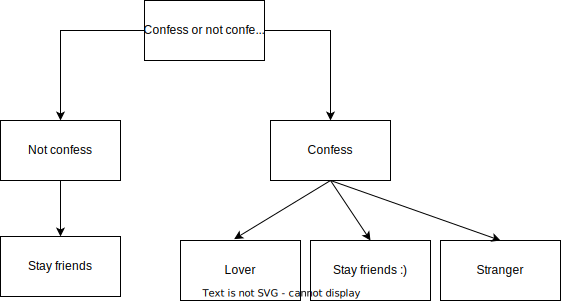
\includegraphics{ea.png}

. . .

jalur kiri (not confess) adalah kepastian, sementara jalur kanan
(confess) adalah kejadian atau aksi berpeluang.

\hypertarget{contoh-lain}{%
\subsection{Contoh lain}\label{contoh-lain}}

\begin{itemize}
\item
  Cuaca besok bisa saja hujan, bisa mendung, dan bisa cerah.
\item
  Kondisi jalan di Jakarta besok pagi bisa macet atau macet banget.
\item
  Nilai ujian anda bisa saja A, B, C, D atau E.
\item
  Melempar dadu bisa muncul angka 1, 2, 3, 4, 5, atau 6.
\end{itemize}

. . .

Seperti yang anda mungkin paham, hampir semua kejadian di dunia ini
adalah kejadian berpeluang.

\hypertarget{notasi-1}{%
\subsection{Notasi}\label{notasi-1}}

\begin{itemize}
\item
  \(S\) (\emph{State}) melambangkan himpunan kemungkinan kejadian.

  \begin{itemize}
  \item
    Lempar koin punya \(S=\{A,G\}\)
  \item
    Lempar dadu punya \(S=\{1,2,3,4,5,6\}\)
  \end{itemize}
\item
  \(P(X)\) melambangkan peluang munculnya kejadian \(X\).

  \begin{itemize}
  \item
    \(P(X=A)\) atau \(P(A)\) artinya peluang munculnya A.
  \item
    \(P(X>3)=\frac{1}{2}\) peluang munculnya angka lebih dari 3 adalah
    \(\frac{1}{2}\).
  \item
    \(P(1\leq X \leq 5)=\) berapa?
  \end{itemize}
\item
  \(P(\bar{A})\) atau \(P(X=\bar{A})\) artinya peluang munculnya
  kejadian selain A.

  \begin{itemize}
  \tightlist
  \item
    Di koin, \(P(\bar{A})=P(G)\)
  \end{itemize}
\end{itemize}

\hypertarget{beberapa-istilah}{%
\subsection{Beberapa istilah}\label{beberapa-istilah}}

\begin{itemize}
\item
  Sebuah himpunan kejadian dikatakan \textbf{adil} (\emph{fair}) jika
  semua anggota \(S\) punya kemungkinan yang sama untuk muncul.

  \begin{itemize}
  \tightlist
  \item
    Dadu yang adil: \(P(1)=P(2)=P(3)=P(4)=P(5)=P(6)=\frac{1}{6}\)
  \end{itemize}
\item
  Sebuah kejadian dikatakan \textbf{independen} jika kejadian tersebut
  tidak tergantung dari kejadian sebelumnya, dan tidak mempengaruhi
  kejadian sesudahnya.

  \begin{itemize}
  \tightlist
  \item
    Jika lemparan pertama keluar 3, lemparan ke-2 tetap punya
    \(P(3)=\frac{1}{6}\), begitupun lemparan ke-3.
  \end{itemize}
\end{itemize}

\hypertarget{menghitung-peluang}{%
\subsection{Menghitung peluang}\label{menghitung-peluang}}

\begin{itemize}
\item
  Pendekatan klasik adalah dengan melakukan eksperimen sebanyak \(n\),
  lalu melihat jumlah dari masing-masing hasilnya.
\item
  Jika ada sebuah koin 2 sisi dengan \(S=\{A,G\}\), maka:
\end{itemize}

\[
P(A)=\frac{n(A)}{n(S)}
\]

\hypertarget{menghitung-peluang-1}{%
\subsection{Menghitung peluang}\label{menghitung-peluang-1}}

\begin{itemize}
\item
  Sebuah koin yang adil dengan dua sisi \(S=\{A,G\}\) dan independen.
\item
  Lempar koin sebanyak \(n=10\), lalu muncul \(A=4\) dan \(G=6\), saya
  katakan:
\end{itemize}

\[
P(A)=\frac{4}{10}
\]

\begin{itemize}
\tightlist
\item
  berapa \(P(G)\)?
\end{itemize}

\hypertarget{rules-dasar}{%
\subsection{Rules dasar}\label{rules-dasar}}

\begin{itemize}
\item
  \(0 \leq P(X) \leq 1\), 0 = gak mungkin, 1 = pasti.
\item
  nilai peluang bermakna limit tak hingga. \(P(X=A)=0,5\) artinya jika
  \(X\) dilakukan berulang kali, frekuensi relatif dari \(X=A\) adalah
  0,5.
\item
  \(P(A \ \text{atau} \ B) = P(A \cup B)=P(A)+P(B)\)
\end{itemize}

Berapa peluang munculnya 1 atau 2 pada lemparan sebuah dadu yang adil?

\begin{itemize}
\tightlist
\item
  \(P(X=1 \cup X=2)=P(X=1)+P(X=2)=\frac{1}{6}+\frac{1}{6}\)
\end{itemize}

\hypertarget{rules-dasar-1}{%
\subsection{Rules dasar}\label{rules-dasar-1}}

\begin{itemize}
\item
  \(P(S_1 \cup S_2 \cup .... S_S)=\sum_{i=1}^S S_i=1\)

  \begin{itemize}
  \item
    koin: \(P(A)+P(G)=1\)
  \item
    dadu: \(P(1)+P(2)+P(3)+P(4)+P(5)+P(6)=1\)
  \end{itemize}
\item
  \(P(\bar{A})=1-P(A)\)

  \begin{itemize}
  \item
    \(P(\bar{X}<3)=P(3)+P(4)+P(5)+P(6)\)
  \item
    \(P(\bar{X}<3)=1-\left(P(1)+P(2) \right)\)
  \end{itemize}
\end{itemize}

\hypertarget{pendekatan-klasik}{%
\subsection{Pendekatan klasik}\label{pendekatan-klasik}}

\begin{itemize}
\item
  Tahun lalu, dari 40 mahasiswa yang mengambil mata kuliah Statistika, 5
  orang dapat nilai A, 10 orang dapat nilai B, 20 orang dapat nilai C, 4
  orang dapat nilai D dan 1 orang dapat nilai E. Berapa persen peluang
  mahasiswa untuk tidak lulus di kelas Statistika?
\item
  \(P(\text{tidak lulus})=P(D)+P(E)=1-P(A \cup B \cup C)\)
\item
  \(P(\text{tidak lulus})=\frac{4+1}{40}=\frac{5}{40}=\frac{1}{8}\)
\end{itemize}

\hypertarget{review}{%
\subsection{Review}\label{review}}

\begin{itemize}
\item
  Kejadian berpeluang adalah suatu kejadian atau aksi yang memiliki
  lebih dari satu kemungkinan hasil (\emph{outcome}) yang didapatkan
  secara acak (\emph{random}).
\item
  Hampir semua kejadian di dunia ini adalah kejadian berpeluang.
\item
  Pendekatan klasik adalah cara paling sederhana menghitung peluang:
  jumlah munculnya \emph{outcome} \(X\) dibagi jumlah experiment \(n\).
\end{itemize}

\hypertarget{expected-value}{%
\subsection{Expected Value}\label{expected-value}}

\begin{itemize}
\item
  Nilai ekspektasi adalah sebuah nilai yang disematkan pada
  probabilitas.
\item
  Merupakan rata-rata nilai yang diantisipasi atas berbagai kemungkinan
  nilai yang muncul dari suatu kejadian berpeluang.
\end{itemize}

\[
EV=\sum P(X_i) \times X_i
\]

\hypertarget{ev-judi}{%
\subsection{EV Judi}\label{ev-judi}}

\begin{itemize}
\item
  Sebuah koin yang adil digunakan sebagai dasar sebuah perjudian. Jika
  keluar A, anda akan mendapatkan Rp 10.000. Jika keluar G, anda harus
  membayar Rp 12.000. Berapa nilai ekspektasi dari perjudian tersebut?
\item
  \(EV=P(A) \times V(A) + P(G) \times V(G)\)
\item
  \(EV=\frac{1}{2} \times 10000 + \frac{1}{2} \times -12000=-1000\)
\end{itemize}

\hypertarget{ev-judi-1}{%
\subsection{EV judi}\label{ev-judi-1}}

\begin{itemize}
\item
  Sebuah dadu yang adil digunakan sebagai dasar sebuah perjudian. Jika
  keluar 1, anda membayar Rp. 20.000. Jika keluar 6, anda mendapatkan Rp
  50.000. Jika keluar ganjil selain 1 anda membayar Rp. 5.000, jika
  keluar genap selain 6, anda mendapatkan Rp.1.000. Hitung nilai
  ekspektasi perjudian tersebut.
\item
  \(EV=\frac{1}{6} \times -20000 + \frac{1}{6} \times 50000 + \frac{2}{6} \times -5000 + \frac{2}{6}\times 1000\)
\item
  \(EV=3666,67\)
\end{itemize}

\hypertarget{memaknai-ev}{%
\subsection{Memaknai EV}\label{memaknai-ev}}

\begin{itemize}
\item
  EV judi koin di atas artinya anda mungkin aja menang 10000 ketika
  sekali ikut. Mungkin juga kalah 12000.
\item
  namun, jika judi tersebut diulang berkali-kali sebanyak mungkin, anda
  akan secara total mendapatkan -1000.
\item
  Logikanya sama jika judi dilakukan 1 kali, tetapi yang ikut judi ada
  banyak orang:

  \begin{itemize}
  \tightlist
  \item
    Jika judi diikuti 1000 orang, akan ada 500 orang menang 10000, tapi
    500 orang lainnya kalah 12000.
  \end{itemize}
\item
  Jika anda bandar, judi mana yang lebih baik?
\end{itemize}

\hypertarget{bandar-judi}{%
\subsection{Bandar judi}\label{bandar-judi}}

\begin{itemize}
\item
  Bandar judi sudah pasti akan membuat judi yang memiliki nilai
  ekspektasi yang negatif bagi peserta judi.
\item
  Di kasus judi koin, jika ada bandar punya 1000 pelanggan:

  \begin{itemize}
  \item
    Dia harus membayar \(10000 \times 500=\) 5 juta.
  \item
    Tapi dapat \(12000 \times 500=\) 6 juta.
  \end{itemize}
\item
  Bandar yang baik tidak akan menjual judi dadu di atas.

  \begin{itemize}
  \tightlist
  \item
    Apa yang akan dilakukan bandar yang baik?
  \end{itemize}
\end{itemize}

\hypertarget{pengambilan-keputusan}{%
\subsection{Pengambilan keputusan}\label{pengambilan-keputusan}}

\begin{itemize}
\item
  EV dapat digunakan sebagai basis pengambilan keputusan.
\item
  Kita dapat membandingkan dua kejadian dan memilih sebuah keputusan
  yang memiliki nilai EV lebih besar.

  \begin{itemize}
  \tightlist
  \item
    jika ada keputusan A dan keputusan B, kita memilih keputusan A jika
    \(EV(A) > EV(B)\)
  \end{itemize}
\item
  Namun Ketika kita melibatkan kejadian berpeluang, pengambilan
  keputusan ini tergantung dari \textbf{profil risiko}.
\end{itemize}

\hypertarget{profil-risiko}{%
\subsection{Profil risiko}\label{profil-risiko}}

\begin{itemize}
\item
  Seseorang dihadapkan dengan sebuah keputusan A dan B. keputusan A
  merupakan sebuah kepastian sementara keputusan B merupakan kejadian
  berpeluang:

  \begin{itemize}
  \item
    Risk neutral ketika orang tsb memilih A ketika \(V(A)>EV(B)\) dan
    memilih B ketika \(V(A)<EV(B)\)
  \item
    Risk averse ketika orang tsb memilih A bahkan ketika \(V(A)<EV(B)\).
  \item
    Risk loving ketika orang tsb memilih B bahkan ketika \(V(A)>EV(B)\).
  \end{itemize}
\end{itemize}

\hypertarget{profil-risiko-1}{%
\subsection{Profil risiko}\label{profil-risiko-1}}

\begin{itemize}
\item
  Lihat kembali judi koin dengan EV=-1.000:

  \begin{itemize}
  \item
    tidak ikut: V=0, ikut: EV=-1.000.
  \item
    orang risk neutral dan risk averse tidak akan ikut judi, sementara
    risk loving akan ikut.
  \end{itemize}
\item
  Lihat kembali judi dadu dengan EV=3.666,67:

  \begin{itemize}
  \item
    tidak ikut: V=0, ikut: EV=3.666,67.
  \item
    orang risk neutral dan risk loving akan ikut, sementara orang risk
    averse tidak akan ikut.
  \end{itemize}
\end{itemize}

\hypertarget{asuransi}{%
\subsection{Asuransi}\label{asuransi}}

\begin{itemize}
\item
  Daerah Jigikirsi merupakan daerah yang cukup rawan dalan kejahatan
  curanmor. Dalam setahun ada setidaknya 1000 kejadian curanmor.
  Asumsikan di jigikirsi ada 10.000 pemilik kendaraan bermotor, dan
  semuanya memiliki harga yang sama yaitu 15 juta rupiah. berapa nilai
  ekspektasi sebuah motor di jigikirsi?
\item
  Hitung probability motor hilang, baru hitung EV.
\end{itemize}

\hypertarget{asuransi-1}{%
\subsection{Asuransi}\label{asuransi-1}}

\begin{itemize}
\item
  Anda menawarkan sebuah produk asuransi yang menjanjikan pergantian
  motor baru jika ada motor hilang di jigikirsi. Berapa premi yang akan
  anda tawarkan ke pemilik motor di jigikirsi?
\item
  Seorang risk neutral akan bayar selama preminya di bawah 1,5 juta.

  \begin{itemize}
  \tightlist
  \item
    premi 1,5 juta disebut juga premi yang adil (fair premium)
  \end{itemize}
\item
  Seorang risk averse akan bayar bahkan ketika premi di atas 1,5 juta.
\item
  Makin besar dia rela bayar, makin besar derajat risk aversenya.
\item
  Risk lovers sebaliknya: baru rela bayar kalo preminya semurah mungkin.
\end{itemize}

\hypertarget{asuransi-2}{%
\subsection{Asuransi}\label{asuransi-2}}

\begin{itemize}
\item
  Sebuah kapal mengirimkan 10.000 kontainer dalam sehari. Dari 10.000
  kontainer tersebut, ada 100 diantaranya rusak saat handling, 50
  diantaranya hilang, dan 65 diantaranya tertahan di pabean, dan 85
  diantaranya salah kirim. Semua kejadian di atas mengakibatkan nilai
  barang anda menjadi 0.
\item
  Berapa premi asuransi yang adil dari kapal tersebut?
\item
  Pebisnis umumnya risk averse. Makanya perusahaan asuransi untung.
\item
  Pejudi biasanya risk loving. Makanya bandar untung.
\end{itemize}

\hypertarget{odds}{%
\subsection{Odds}\label{odds}}

\begin{itemize}
\item
  Odds merupakan sebuah imbal judi yang dibuat sedemikian sehingga
  penjudi memasang taruhan yang seimbang.
\item
  Pada perjudian tebak pemenang / tebak skor, seringkali peserta yang
  bertanding memiliki kemampuan yang berbeda-beda.
\item
  Akibatnya, kemungkinan menangnya juga beda-beda.
\item
  Sering terjadi di judi bole, e-sports, pacuan kuda, dan lain
  sebagainya.
\end{itemize}

\hypertarget{odds-1}{%
\subsection{Odds}\label{odds-1}}

\begin{itemize}
\item
  Misalnya pertandingan Manchester City vs Arema. Jika tim yang anda
  pasang menang, anda dapat uang 2x lipat. Ke mana sebagian besar orang
  akan pasang?
\item
  Karena itu ada yang disebut odds: tim yang kemungkinan menang lebih
  besar akan dapat multiplier / hadiah yang lebih kecil ketimbang tim
  yang kemungkinan menangnya lebih kecil.
\item
  Odds diset sedemikian sehingga jumlah nilai taruhannya akan seimbang.
\end{itemize}

\hypertarget{odds-2}{%
\subsection{Odds}\label{odds-2}}

\includegraphics{bet.jpg}

\begin{itemize}
\item
  Jika anda bet 1 juta ke RBL dan RBL menang, anda akan dapat 5 juta.
  Bet ONIC dan menang, dapat 1 juta 110 ribu.
\item
  Tim mana yang diunggulkan?
\end{itemize}

\hypertarget{odds-3}{%
\subsection{Odds}\label{odds-3}}

\begin{itemize}
\tightlist
\item
  Jika ikut judi dan bayar 1 juta, maka anda akan indifferent jika:
\end{itemize}

\[
P(\text{RBL menang}) \times \text{Odds RBL menang} = \\ P(\text{RBL kalah}) \times \text{Odds RBL kalah}
\]

\begin{itemize}
\tightlist
\item
  Bagi bandar, kemungkinan menang RBL adalah sekitar 18,17\%. ONIC
  berapa?
\end{itemize}

\hypertarget{review-1}{%
\subsection{Review}\label{review-1}}

\begin{itemize}
\item
  Peluang digunakan untuk menghitung expected value.
\item
  Expected value memiliki banyak aplikasi seperti di perjudian dan
  asuransi.
\item
  Odds digunakan untuk menyeimbangkan pasang taruhan. Tapi perlu diingat
  kemungkinan \emph{fraud}.
\end{itemize}

\hypertarget{minggu-depan}{%
\subsection{Minggu depan}\label{minggu-depan}}

\begin{itemize}
\item
  Kejadian berulang, kejadian bersyarat, dan kaidah Bayes.
\item
  Distribusi probabilitas.
\end{itemize}

\hypertarget{pertemuan-7}{%
\section{Pertemuan 7}\label{pertemuan-7}}

\hypertarget{minggu-lalu-1}{%
\subsection{Minggu lalu}\label{minggu-lalu-1}}

\begin{itemize}
\tightlist
\item
  Peluang independen \& pendekatan klasik.
\end{itemize}

\hypertarget{next-1}{%
\paragraph{Next}\label{next-1}}

\begin{itemize}
\tightlist
\item
  Peluang gabungan dan bayesian.
\item
  uji normalitas dan probabilitas sampel
\end{itemize}

\hypertarget{tindakan-ganda}{%
\subsection{Tindakan Ganda}\label{tindakan-ganda}}

\begin{itemize}
\item
  Lemparan 2 koin secara bersamaan memiliki kemungkinan hasil:
\item
  \(S=\{AA,AG,GA,GG\}\)
\item
  Kejadian berganda memiliki rumus:
\item
  \(n_k=n_1 \times n_2 \times n_3 \times ... \times n_k\)
\item
  di mana \(k\) adalah jumlah kejadian individu.
\item
  Berapa \(S\) kalau kita melempar 2 buah dadu?
\end{itemize}

\hypertarget{rules-baru}{%
\subsection{Rules baru}\label{rules-baru}}

\begin{itemize}
\item
  Peluang independen gabungan/beririsan: peluang munculnya A DAN B.
\item
  \(P(A \ \text{dan} \ B)=P(A\&B) = P(A \cap B) = P(A) \times P(B)\)
\item
  Berapa peluang munculnya A dan A dalam lemparan 2 koin adil?
\item
  Berapa peluang munculnya King Hati dalam tarikan 1 deck kartu?
\item
  Berapa peluang munculnya 1 dan ganjil dalam lemparan 2 dadu adil?
\end{itemize}

\hypertarget{rules-baru-1}{%
\subsection{Rules baru}\label{rules-baru-1}}

\begin{itemize}
\item
  Peluang kejadian bersyarat: peluang munculnya A jika B terjadi.
\item
  Perhitungan munculnya outcome A dan B jadi beda rumus seandainya
  kejadian B dipengaruhi oleh kejadian A.
\item
  \(P(A \cap B)=P(A) \times P(B|A)\)
\item
  Jika kejadian independen, maka \(P(B|A)= P(B)\)
\end{itemize}

\hypertarget{lotre}{%
\subsection{Lotre}\label{lotre}}

\begin{itemize}
\item
  Sebuah kotak undian berisi 100 tiket. 50 diantaranya tiket zonk, 30
  diantaranya tiket uang tunai 100 ribu rupiah, 10 diantaranya tiket 200
  ribu rupiah, 8 diantaranya tiket 300 ribu dan 2 tiket 500 ribu rupiah.
  Berapa peluang seseorang bisa ambil tiket 500 ribu 2x berturut-turut?
  (1) jika tiket dikembalikan, (2) jika tiket tidak dikembalikan.
\item
  \begin{enumerate}
  \def\labelenumi{(\arabic{enumi})}
  \tightlist
  \item
    \(P(A \cap B)=P(A) \times P(B)= \frac{2}{100} \times \frac{2}{100} = \frac{4}{10000}\)
  \end{enumerate}
\item
  \begin{enumerate}
  \def\labelenumi{(\arabic{enumi})}
  \setcounter{enumi}{1}
  \tightlist
  \item
    \(P(A \cap B)=P(A) \times P(B|A)= \frac{2}{100} \times \frac{1}{99} = \frac{2}{9900}\)
  \end{enumerate}
\item
  Jika narik lotre ini bayar 90 ribu rupiah, orang risk neutral ikut ga?
\end{itemize}

\hypertarget{kejadian-beririsan}{%
\subsection{Kejadian beririsan}\label{kejadian-beririsan}}

\begin{itemize}
\item
  Sebuah deck terdiri dari 52 kartu standar. Berapa kemungkinan tarikan
  pertama anda dapat lambang hati atau as?
\item
  \(P(💗 \cup A)=P(💗)+P(A)-P(💗 \cap A)=\frac{13}{52}+\frac{4}{52}-\frac{1}{52}\)
\item
  \(P(💗 \cap A) \neq 0\) karena ada 1 kartu yang adalah As dan juga
  berlambang hati.
\end{itemize}

\hypertarget{kejadian-beririsan-1}{%
\subsection{Kejadian beririsan}\label{kejadian-beririsan-1}}

\begin{itemize}
\item
  Ada 140 anak yang saat ini mengambil kelas statistik. 100 diantaranya
  anak-anak yang rupawan. 50 diantaranya anak-anak yang pinter. Berapa
  probabilitas jika saya ambil 1 anak, saya dapat anak yang rupawan atau
  pinter?
\item
  \(P(R \cup P)=P(R)+P(P)=\frac{150}{140}\)?
\item
  Apakah ga mungkin? Masalahnya, ada anak yang pinter DAN rupawan.
  Misalnya yg rupawan \& pinter = 40 orang.
\item
  \(P(R \cup P)=P(R)+P(P)-P(R\cap P)=\frac{100+50-40}{140}=\frac{110}{140}\)
\end{itemize}

\hypertarget{kejadian-beririsan-2}{%
\subsection{Kejadian beririsan}\label{kejadian-beririsan-2}}

\begin{itemize}
\tightlist
\item
  kejadian beririsan dapat diilustrasikan dengan \textbf{diagram venn}.
\end{itemize}

\includegraphics{index_files/figure-pdf/unnamed-chunk-11-1.pdf}

\begin{Shaded}
\begin{Highlighting}[]
\NormalTok{wew}
\end{Highlighting}
\end{Shaded}

\begin{verbatim}
(polygon[GRID.polygon.560], polygon[GRID.polygon.561], polygon[GRID.polygon.562], polygon[GRID.polygon.563], text[GRID.text.564], text[GRID.text.565], text[GRID.text.566], text[GRID.text.567], text[GRID.text.568]) 
\end{verbatim}

\hypertarget{kejadian-beririsan-3}{%
\subsection{Kejadian beririsan}\label{kejadian-beririsan-3}}

\begin{itemize}
\item
  Sebuah acara sosialisasi mengundang 120 orang. Dari data, diketahui
  100 diantaranya beragama islam. Berbekal pengetahuan tersebut, panitia
  mempersiapkan 20 kotak makan siang. Pas break siang, panitia
  mengumumkan ``bagi yang tidak puasa bisa ambil makan siang di meja
  panitia''. Ternyata ada 15 orang yang tidak kebagian. Berapa banyak
  yang tidak puasa? Apa kesalahan dari panitia?
\item
  \(P(Maksi)=1-P(Muslim)+P(Muslim \ \cap \ Maksi)\)
\item
  Panitia mengasumsikan bahwa \(P(Muslim \ \cap \ Maksi) = 0\).
\end{itemize}

\hypertarget{permutasi-dan-kombinasi}{%
\subsection{Permutasi dan Kombinasi}\label{permutasi-dan-kombinasi}}

\begin{itemize}
\item
  Jika kita perlu menghitung ada berapa cara untuk mendapatkan \(r\)
  keluaran dari total kemungkinan \(n\) keluaran, kita dapat menggunakan
  permutasi dan kombinasi.
\item
  Permutasi jika urutan ngaruh. \(ABC \neq BCA\)
\end{itemize}

\[
P^n_r=\frac{n!}{(n-r)!}
\]

\begin{itemize}
\tightlist
\item
  Kombinasi jika urutan ga ngaruh. \(ABC=BCA\)
\end{itemize}

\[
C^n_r=\frac{n!}{r!(n-r)!}
\]

\hypertarget{faktorial}{%
\subsection{Faktorial}\label{faktorial}}

\begin{itemize}
\item
  Tanda seru setelah angka disebut juga dengan faktorial.
\item
  Faktorial mirip dengan pangkat, tapi dikali berkurang terus hingga 1.
\item
  \(3!=3\times 2\times 1\)
\item
  \(6!=6\times 5\times 4 \times 3 \times 2 \times 1=6 \times 5 \times 4 \times 3!\)
\item
  \(\frac{6!}{3!}=\frac{6 \times 5 \times 4 \times 3!}{3!}=6 \times 5 \times 4\)
\end{itemize}

\hypertarget{permutasi}{%
\subsection{Permutasi}\label{permutasi}}

\begin{itemize}
\item
  Sebuah ujian terdiri dari total 10 soal. Namun, setiap mahasiswa hanya
  akan mengerjakan 4 soal saja yang muncul secara acak dari 10 soal
  tersebut. Ada berapa tipe soal yang mungkin muncul di ujian tersebut?
\item
  Jika beda urutan diitung 1 tipe soal, maka
\item
  \[P^{10}_4=\frac{10!}{(10-4)!}=\frac{10!}{6!}=5040\]
\end{itemize}

\hypertarget{kombinasi}{%
\subsection{Kombinasi}\label{kombinasi}}

\begin{itemize}
\item
  Sebuah ujian terdiri dari total 10 soal. Namun, setiap mahasiswa hanya
  akan mengerjakan 4 soal saja yang muncul secara acak dari 10 soal
  tersebut. Ada berapa tipe soal yang mungkin muncul di ujian tersebut?
\item
  Jika beda urutan soal diitung tipe yang sama, maka
\item
  \[C^{10}_4=\frac{10!}{4!(10-4)!}=\frac{10!}{4!6!}=\frac{10\times9\times 8\times 7}{4 \times 3\times 2\times 1}=210\]
\end{itemize}

\hypertarget{permutasi-1}{%
\subsection{Permutasi}\label{permutasi-1}}

\begin{itemize}
\item
  Sebuah kotak berisi 12 bola merah, 13 bola biru dan 15 bola hijau.
  Pengambilan bola tidak dikembalikan. Hitung kemungkinan pengambilan
  pertama bola merah, bola ke-2 hijau, dan bola ke-3 biru.
\item
  Pertanyaan ini dapat dijawab dengan 2 cara. Pertama, cara klasik:
\item
  \(P(R_1G_2B_3)=P(R) \times P(G|R) \times P(B|R_1G_2)=\frac{12}{40} \times \frac{15}{39} \times \frac{13}{38}\)
\item
  \(P(R_1G_2B_3) \approx 0,04\)
\end{itemize}

\hypertarget{permutasi-2}{%
\subsection{Permutasi}\label{permutasi-2}}

\begin{itemize}
\tightlist
\item
  Cara ke-2 dengan menggunakan permutasi:
\end{itemize}

\[
P(R_1G_2B_3)=\frac{P^{12}_1P^{15}_1P^{13}_1}{P^{40}_3}=\frac{\frac{12!}{11!}\times\frac{15!}{14!}\times\frac{13!}{12!}}{\frac{40!}{37!}}=\frac{2340}{59280} \approx 0,04
\]

\hypertarget{kombinasi-1}{%
\subsection{Kombinasi}\label{kombinasi-1}}

\begin{itemize}
\item
  Sebuah kotak berisi 12 bola merah, 13 bola biru dan 15 bola hijau.
  Pengambilan bola tidak dikembalikan. Hitung kemungkinan 3 kali
  pengambilan akan dapat warna yang berbeda-beda.
\item
  Dengan cara klasik dapat dilakukan, namun perlu dipertimbangkan ada
  berapa kemungkinan 3 warna berbeda-beda.
\item
  \(P(RGB)=3! \times P(R_1G_2B_3)\approx6\times0,04\approx0,24\)
\end{itemize}

\hypertarget{kombinasi-2}{%
\subsection{Kombinasi}\label{kombinasi-2}}

\begin{itemize}
\tightlist
\item
  Cara ke-2 dengan menggunakan kombinasi:
\end{itemize}

\[
P(RGB)=\frac{C^{12}_1C^{15}_1C^{13}_1}{C^{40}_3}=\frac{\frac{12!}{11!}\times\frac{15!}{14!}\times\frac{13!}{12!}}{\frac{40!}{3!37!}}=\frac{2340}{9880}\approx0,24.
\]

\hypertarget{diagram-pohon}{%
\subsection{Diagram pohon}\label{diagram-pohon}}

\begin{figure}[H]

{\centering \includegraphics[width=20.66in,height=3.15in]{index_files/figure-latex/mermaid-figure-1.png}

}

\end{figure}

\hypertarget{probabilitas-marjinal}{%
\subsection{Probabilitas marjinal}\label{probabilitas-marjinal}}

\begin{itemize}
\item
  Sebuah perusahaan handphone memesan layar dari 3 perusahaan yang
  berbeda, yaitu A,B dan C. Perusahaan A menyuplai 270 layar, B
  menyuplai 320 layar, C menyuplai 110 layar. Si perusahaan
  mengantisipasi kemungkinan \emph{defect} dari A sebesar 0,015, B
  sebesar 0,02, C sebesar 0,03. Berapa probabilitas layar di perusahaan
  ini \emph{defect}?
\item
  \(P(D)=\sum_S P(X) \times P(D|X)\)
\item
  \(P(D)=\frac{270}{700} \times 0,015 + \frac{320}{700} \times 0,02 \frac{110}{700} \times 0,03\)
\item
  \(P(D)=0,0196 \approx 0,02\)
\end{itemize}

\hypertarget{bayesian-probability}{%
\subsection{Bayesian Probability}\label{bayesian-probability}}

\begin{itemize}
\tightlist
\item
  Seorang peneliti bernama Bayes menemukan sebuah rumus yang menunjukkan
  hubungan antara peluang kondisional:
\end{itemize}

\[
P(A|B)=\frac{P(B|A) \times P(A)}{P(B)}
\]

\begin{itemize}
\tightlist
\item
  Kemungkinan munculnya A jika B terjadi tidak sama dengan kemungkinan
  mmunculnya B jika A terjadi.
\end{itemize}

\hypertarget{bayesian}{%
\subsection{Bayesian}\label{bayesian}}

\begin{itemize}
\item
  Lihat soal sebelumnya. ditemukan bahwa ada 1 produk cacat /
  \emph{defect}, berapa kemungkinannya produk tersebut datang dari
  supplier A?
\item
  \(A=\) produk berasal dari supplier A, \(D=\) produk cacat.
\item
  \(P(A|D)=\frac{P(D|A) \times P(A)}{P(D)}=\frac{0,015 \times \frac{270}{700}}{0,0216}\)
\item
  \(P(A|D)=0,295 \approx 0,3\)
\item
  Produk cacat tersebut paling mungkin datang dari supplier mana?
\end{itemize}

\hypertarget{bayesian-1}{%
\subsection{Bayesian}\label{bayesian-1}}

\begin{itemize}
\item
  \(P(B|D)=\frac{P(D|B) \times P(B)}{P(D)}=\frac{0,02 \times \frac{320}{700}}{0,0216}=0,465\)
\item
  \(P(C|D)=\frac{P(D|C) \times P(C)}{P(D)}=\frac{0,03 \times \frac{110}{700}}{0,0216}=0,24\)
\item
  \(P(D|C)\) paling besar, tapi order datang paling banyak dari
  perusahaan B. Karena itu, kemungkinan barang rusak itu datang dari B
  juga jadi lebih besar.
\end{itemize}

\hypertarget{bayesian-2}{%
\subsection{Bayesian}\label{bayesian-2}}

\begin{itemize}
\item
  Tesle, sebuah perusahaan mobil listrik, tertarik investasi di negara
  Wikindi karena ada program insentif. Namun Wikindi mau pilpres dengan
  3 calon. Calon A punya kans 90\% akan melanjutkan program insentif.
  Calon B sekitar 50\%, dan Calon C sangat anti program tsb dan hanya
  akan lanjutkan sekitar 10\% kans. Berdasarkan survey, Kemungkinan
  menang calon A,B dan C adalah 25\%,35\% dan 40\%.
\item
  Jika Tesle tidak peduli siapa presidennya nanti, berapa \% kans
  program insentif akan diteruskan?
\item
  Jika akhirnya program tidak diteruskan, tentukan berapa \% kemungkinan
  akhirnya yang menang calon A, calon B dan calon C.
\end{itemize}

\hypertarget{pertemuan-8}{%
\section{Pertemuan 8}\label{pertemuan-8}}

\hypertarget{data-dan-statistika}{%
\subsection{Data dan Statistika}\label{data-dan-statistika}}

\begin{itemize}
\item
  Data adalah \textbf{kumpulan informasi yang didapatkan dari melakukan
  pengamatan (observasi)}.
\item
  Pada hakikatnya, penggunaan data dan statistika berfungsi untuk
  \textbf{menjawab pertanyaan} seperti:

  \begin{itemize}
  \item
    Bagaimana kondisi sosial ekonomi penduduk Indonesia? Dibandingkan
    dengan RRT?
  \item
    Berapa ekspor Indonesia tahun 2020? Apakah meningkat dibandingkan
    tahun 2019?
  \end{itemize}
\item
  Anda setiap hari juga mengumpulkan data!
\end{itemize}

\hypertarget{data-yang-baik}{%
\subsection{Data yang baik}\label{data-yang-baik}}

\begin{itemize}
\item
  Data akan menjadi basis dalam menjawab pertanyaan dan membuat
  keputusan. Data salah, keputusan juga salah!
\item
  Data yang baik haruslah objektif, representatif, valid, tepat waktu
  dan relevan.
\item
  Objektif berarti dapat meminimalisir perbedaan persepsi antar-pengamat
  / individu.
\item
  harus memiliki alat ukur yang konsisten dan disepakati, dengan metode
  yang dapat diaudit.
\item
  contoh: di kelas saya ada 10 orang yang gendut vs di kelas saya, 10
  orang punya berat badan di atas 70 kg.
\end{itemize}

\hypertarget{data-yang-baik-1}{%
\subsection{Data yang baik}\label{data-yang-baik-1}}

\begin{itemize}
\item
  Representatif berarti harus mewakili obyek yang diamati. Obyek yang
  representatif biasanya akan didapatkan dengan sampling yang acak.
\item
  valid berarti data tersebut memiliki kesalahan sampling yang kecil dan
  memiliki tingkat ketelitian yang tinggi. Jika diulang samplingnya,
  hasilnya akan sama.
\item
  tepat waktu berarti datanya harus sesuai berdasarkan waktu dan selalu
  terupdate.
\item
  relevan berarti data tersebut benar-benar mengukur hal yang sesuai
  dengan pertanyaan yang ingin dijawab.
\end{itemize}

\hypertarget{jenis-jenis-data}{%
\subsection{Jenis-jenis data}\label{jenis-jenis-data}}

\begin{longtable}[]{@{}
  >{\raggedright\arraybackslash}p{(\columnwidth - 4\tabcolsep) * \real{0.2941}}
  >{\raggedright\arraybackslash}p{(\columnwidth - 4\tabcolsep) * \real{0.2941}}
  >{\raggedright\arraybackslash}p{(\columnwidth - 4\tabcolsep) * \real{0.4118}}@{}}
\toprule\noalign{}
\begin{minipage}[b]{\linewidth}\raggedright
jenis data
\end{minipage} & \begin{minipage}[b]{\linewidth}\raggedright
definisi
\end{minipage} & \begin{minipage}[b]{\linewidth}\raggedright
contoh
\end{minipage} \\
\midrule\noalign{}
\endhead
\bottomrule\noalign{}
\endlastfoot
Kategorikal / nominal & kualitatif, ga ada urutan & nama, jenis kelamin,
suku \\
Ordinal & kualitatif, ada urutan & ukuran baju, ukuran sepatu, medali \\
Hitung & kuantitatif, integer & nomor telepon, jumlah anak \\
Riil / kontinyu & kuantitatif, riil & PDB, ekspor impor \\
\end{longtable}

\hypertarget{data-kontinyu}{%
\subsection{Data Kontinyu}\label{data-kontinyu}}

\begin{itemize}
\item
  data kontinyu dapat dibagi 2: rasio dan interval.
\item
  keduanya memiliki interval yang sama untuk semua angka.
\item
  tapi, interval tidak punya 0 yang berarti.

  \begin{itemize}
  \item
    untuk rasio, 0 = tidak ada. contoh: ekspor, impor, kalori. Tidak ada
    nilai negatif.
  \item
    interval, 0 = ga penting. contoh: nilai TOEFL, temperatur. Ada nilai
    negatif.
  \end{itemize}
\item
  Transformasi di rasio tidak akan mengubah besarnya urutan.

  \begin{itemize}
  \item
    10 kg = 2x lebih berat dari 5 kg. begitupun 22.04 lbs vs 11.02 lbs
  \item
    1\(^o\) C to 100\(^o\) C = 100x lipat, tapi 274.15\(^o\) K to
    373.15\(^o\) K bukan 100x lipat
  \end{itemize}
\end{itemize}

\hypertarget{dampaknya}{%
\subsection{Dampaknya?}\label{dampaknya}}

\begin{itemize}
\item
  Tipe data yang berbeda menuntut cara analisis yang berbeda pula.
\item
  Biasanya, dalam metode statistik, data rasio adalah data yang paling
  mudah untuk digunakan dalam analisis.
\item
  Jika tipe data anda bukan rasio, harus sedikit diakalin metodenya.
  Bisa, tapi lebih ribet dikit.
\item
  Di mata kuliah ini, kita akan fokus pada data yang sebagian besar
  berupa data rasio.
\end{itemize}

\hypertarget{cara-pengambilan-data}{%
\subsection{Cara pengambilan data}\label{cara-pengambilan-data}}

\begin{itemize}
\item
  \textbf{Sensus} adalah metode pengumpulan data yang melibatkan
  keseluruhan populasi yang ingin diselidiki.

  \begin{itemize}
  \tightlist
  \item
    misalnya, untuk mendapatkan nilai UAS mata kuliah statistika, saya
    mencatat semua nilai UAS mahasiswa APP yang mengambil mata kuliah
    statistika.
  \end{itemize}
\item
  Sensus memiliki gambaran yang lengkap, tapi anda tidak boleh
  menyimpulkan sesuatu dari luar populasi.

  \begin{itemize}
  \tightlist
  \item
    misalnya, hasil sensus penduduk jagakarsa tidak dapat anda gunakan
    untuk menyimpulkan Jakarta Selatan secara umum.
  \end{itemize}
\item
  Kelemahan sensus: mahal dan makan banyak waktu.
\end{itemize}

\hypertarget{cara-pengambilan-data-1}{%
\subsection{Cara pengambilan data}\label{cara-pengambilan-data-1}}

\begin{itemize}
\item
  \textbf{sampling} adalah metode pengumpulan data yang melibatkan
  sebagian dari populasi yang ingin diselidiki.

  \begin{itemize}
  \item
    misalnya, untuk menilai apakah kelas A lebih bagus nilainya dari
    kelas B, saya menguji 10 orang dari kelas A dan 10 orang dari kelas
    B.
  \item
    10 orang ini kita sebut sampel, sementara populasinya adalah
    keseluruhan anggota kelas A dan kelas B.
  \end{itemize}
\item
  sampling lebih murah, namun kita harus memastikan bahwa samplenya
  \textbf{representatif}.
\end{itemize}

\hypertarget{sampling}{%
\subsection{Sampling}\label{sampling}}

\begin{itemize}
\item
  dapat dilakukan secara \textbf{acak} dan \textbf{non-acak}.
\item
  Acak (\emph{random}) artinya bahwa semua anggota populasi punya
  kesempatan yang sama untuk menjadi sampel.

  \begin{itemize}
  \tightlist
  \item
    misalnya saya tunjuk secara acak 10 mahasiswa di tiap kelas.
  \end{itemize}
\item
  Non-acak berarti kita mendorong satu bagian dari populasi dengan
  karakteristik tertentu punya kesempatan yang lebih banyak untuk
  terpilih menjadi sampel.

  \begin{itemize}
  \tightlist
  \item
    misalnya saya hanya menunjuk 10 anak yang pakai kacamata, atau
    menunjuk 10 anak yang duduknya paling dekat saya.
  \end{itemize}
\end{itemize}

\hypertarget{acak-atau-jangan}{%
\subsection{Acak atau jangan?}\label{acak-atau-jangan}}

\begin{itemize}
\item
  Idealnya adalah kita punya data populasi. Tapi biasanya impractical.
\item
  Jika harus pakai sampel, maka sampel yang terbaik adalah sampel yang
  \textbf{representatif}.
\item
  Sebuah sampel kita anggap representatif jika sampel tersebut punya
  karakteristik yang kita yakini mendekati populasi aslinya.
\end{itemize}

\hypertarget{representatif}{%
\subsection{Representatif}\label{representatif}}

\begin{itemize}
\item
  Volume darah dalam tubuh manusia biasanya sekitar 5 liter. Untuk
  ngetes diabetes, diambil 0,5 ml sampel saja, gak diambil semua.
\item
  Kenapa? Karena 0,5 ml darah ini mewakili kesemua darah di tubuh
  manusia. Jika 0,5 liter ini terdeteksi diabetes, maka yang di tubuh
  juga pasti diabetes.
\item
  Demokrasi juga sama: dari total 270 juta manusia di Indonesia,
  dianggap ada 550 orang yang bisa mewakili.
\end{itemize}

\hypertarget{representatif-1}{%
\subsection{Representatif}\label{representatif-1}}

\begin{itemize}
\item
  Karakteristik data yang kita lihat umumnya adalah \textbf{tendensi
  sentral}, \textbf{sebaran} dan \textbf{distribusi}.
\item
  Sebuah sampel yang representatif harusnya memiliki rata-rata, standar
  deviasi dan bentuk distribusi yang serupa dengan aslinya.
\item
  Misalnya seluruh mahasiswa PIWAR 2 sejumlah 150 orang punya rata-rata
  UTS 70 dengan rentang 15.
\item
  Jika saya ambil sampel 15 orang lalu saya tes lagi, maka 15 orang itu
  harus punya rata-rata dan rentang yang sama.
\end{itemize}

\hypertarget{random}{%
\subsection{Random}\label{random}}

\begin{itemize}
\item
  Sampling yang diambil secara acak akan memiliki kemungkinan
  representatif yang tinggi dibanding disaring (misalnya, 15 orang ini
  hanya saya pilih yang nilainya paling tinggi).
\item
  Tidak hanya nilai, tapi juga karakteristik lain: jika cewe:cowo di
  PIWAR = 70:30, maka sampelnya juga akan punya perbandingan yang sama.
  Juga karakteristik-karakteristik lainnya.
\item
  Next time kita akan belajar tendensi sentral, rentang dan distribusi
  lebih jauh.
\end{itemize}

\hypertarget{sampling-acak}{%
\subsection{Sampling acak}\label{sampling-acak}}

\begin{itemize}
\item
  Simple random sampling berarti mengambil sampel secara acak langsung
  dari populasinya.
\item
  Stratified random sampling: membagi populasi menjadi sub-populasi atau
  strata, lalu mengambil secara acak dari tiap-tiap stratum.
\item
  Cluster random sampling: membagi populasi menjadi strata, lalu secara
  acak mengambil satu stratum dan mengambil semua anggota stratum
  tersebut menjadi sampel.
\item
  Multistage random sampling: Membagi populasi ke dalam strata,
  mengambil beberapa strata secara acak, lalu dari strata yang diambil
  tersebut disampling lagi.
\end{itemize}

\hypertarget{pilih-yang-mana}{%
\subsection{Pilih yang mana?}\label{pilih-yang-mana}}

\begin{itemize}
\item
  Semua teknik di atas dapat dilakukan dengan kemungkinan mendapatkan
  sample representatif yang relatif mirip.
\item
  Tapi intinya, harus dilakukan secara acak!
\item
  Semakin besar populasinya, biasanya menggunakan strata bisa lebih
  membuat percaya diri.
\item
  tapi jika benar dapat melakukannya secara acak, maka seharusnya cara
  manapun akan memiliki data yang tidak berbeda jauh.
\end{itemize}

\hypertarget{statistika}{%
\subsection{Statistika}\label{statistika}}

\begin{itemize}
\item
  Statistika adalah ilmu yang mempelajari bagaimana cara mengumpulkan,
  mengorganisasikan, menerjemahkan dan menarik kesimpulan dari data.
\item
  Meskipun statistika awalnya banyak diajarkan untuk bidang ilmu pasti,
  namun saat ini ekonomi dan manajemen juga menggunakannya.
\item
  Cara-cara menerjemahkan dan menarik kesimpulan ini juga tergantung
  dari jenis data yang kita perlukan.
\end{itemize}

\hypertarget{pertemuan-9}{%
\section{Pertemuan 9}\label{pertemuan-9}}

\hypertarget{minggu-lalu-2}{%
\subsection{Minggu lalu}\label{minggu-lalu-2}}

\begin{itemize}
\item
  Berbagai jenis data: kategorikal, ordinal, diskrit dan kontinyu.
\item
  survey: random dan non-random
\end{itemize}

\hypertarget{minggu-ini}{%
\paragraph{Minggu ini}\label{minggu-ini}}

\begin{itemize}
\tightlist
\item
  Distribusi frekuensi dan statistik deskriptif
\end{itemize}

\hypertarget{distribusi-frekuensi}{%
\subsection{Distribusi frekuensi}\label{distribusi-frekuensi}}

\begin{itemize}
\item
  Distribusi frekuensi adalah cara yang paling awal dilakukan untuk
  mendapatkan gambaran dari suatu sampel / populasi.
\item
  Kita membutuhkan distribusi frekuensi karena sebagai manusia biasa
  kita ga akan sanggup membaca semua data poin 1 1.
\item
  Perlu semacam alat ukur yang menggambarkan semua data yang kita punya.
\end{itemize}

\hypertarget{distribusi-kualitatif}{%
\subsection{Distribusi kualitatif}\label{distribusi-kualitatif}}

\begin{itemize}
\tightlist
\item
  Misalnya anda melakukan survey merk handphone yang dimiliki saat ini
  dengan sample 50 orang.
\end{itemize}

\begin{Shaded}
\begin{Highlighting}[]
\FunctionTok{library}\NormalTok{(tidyverse)}
\FunctionTok{library}\NormalTok{(kableExtra)}
\end{Highlighting}
\end{Shaded}

\begin{verbatim}

Attaching package: 'kableExtra'
\end{verbatim}

\begin{verbatim}
The following object is masked from 'package:dplyr':

    group_rows
\end{verbatim}

\begin{Shaded}
\begin{Highlighting}[]
\FunctionTok{sample}\NormalTok{(}\AttributeTok{x=}\FunctionTok{c}\NormalTok{(}\StringTok{"Apple"}\NormalTok{,}\StringTok{"Samsung"}\NormalTok{,}\StringTok{"Oppo"}\NormalTok{,}\StringTok{"Vivo"}\NormalTok{,}\StringTok{"Xiaomi"}\NormalTok{,}\StringTok{"Lainnya"}\NormalTok{),}
                      \AttributeTok{prob=}\FunctionTok{c}\NormalTok{(}\FloatTok{0.1}\NormalTok{,}\FloatTok{0.3}\NormalTok{,}\FloatTok{0.15}\NormalTok{,}\FloatTok{0.13}\NormalTok{,}\FloatTok{0.17}\NormalTok{,}\FloatTok{0.15}\NormalTok{),}
                      \AttributeTok{size=}\DecValTok{50}\NormalTok{,}
                      \AttributeTok{replace =} \ConstantTok{TRUE}\NormalTok{)}
\end{Highlighting}
\end{Shaded}

\begin{verbatim}
 [1] "Lainnya" "Lainnya" "Xiaomi"  "Vivo"    "Lainnya" "Lainnya" "Lainnya"
 [8] "Apple"   "Oppo"    "Lainnya" "Vivo"    "Samsung" "Vivo"    "Lainnya"
[15] "Xiaomi"  "Xiaomi"  "Samsung" "Lainnya" "Oppo"    "Samsung" "Samsung"
[22] "Vivo"    "Lainnya" "Vivo"    "Lainnya" "Samsung" "Samsung" "Xiaomi" 
[29] "Oppo"    "Samsung" "Samsung" "Samsung" "Samsung" "Vivo"    "Samsung"
[36] "Vivo"    "Samsung" "Apple"   "Oppo"    "Oppo"    "Lainnya" "Samsung"
[43] "Lainnya" "Samsung" "Vivo"    "Oppo"    "Vivo"    "Xiaomi"  "Apple"  
[50] "Lainnya"
\end{verbatim}

\begin{itemize}
\item
  Cara mengolahnya secara manual adalah dengan menggunakan
  \textbf{Tally}
\item
  Informasi apa yang menarik dari tabel ini?
\end{itemize}

\hypertarget{distribusi-kualitatif-1}{%
\subsection{Distribusi kualitatif}\label{distribusi-kualitatif-1}}

\begin{itemize}
\tightlist
\item
  Gimana kalau datanya ada 1000?
\end{itemize}

\begin{Shaded}
\begin{Highlighting}[]
\FunctionTok{library}\NormalTok{(tidyverse)}
\FunctionTok{library}\NormalTok{(kableExtra)}
\NormalTok{dat}\OtherTok{\textless{}{-}}\FunctionTok{as.tibble}\NormalTok{(}\FunctionTok{sample}\NormalTok{(}\AttributeTok{x=}\FunctionTok{c}\NormalTok{(}\StringTok{"Apple"}\NormalTok{,}\StringTok{"Samsung"}\NormalTok{,}\StringTok{"Oppo"}\NormalTok{,}\StringTok{"Vivo"}\NormalTok{,}\StringTok{"Xiaomi"}\NormalTok{,}\StringTok{"Lainnya"}\NormalTok{),}
                      \AttributeTok{prob=}\FunctionTok{c}\NormalTok{(}\FloatTok{0.1}\NormalTok{,}\FloatTok{0.3}\NormalTok{,}\FloatTok{0.15}\NormalTok{,}\FloatTok{0.13}\NormalTok{,}\FloatTok{0.17}\NormalTok{,}\FloatTok{0.15}\NormalTok{),}
                      \AttributeTok{size=}\DecValTok{1000}\NormalTok{,}
                      \AttributeTok{replace =} \ConstantTok{TRUE}\NormalTok{))}
\end{Highlighting}
\end{Shaded}

\begin{verbatim}
Warning: `as.tibble()` was deprecated in tibble 2.0.0.
i Please use `as_tibble()` instead.
i The signature and semantics have changed, see `?as_tibble`.
\end{verbatim}

\begin{Shaded}
\begin{Highlighting}[]
\FunctionTok{kbl}\NormalTok{(dat) }\SpecialCharTok{\%\textgreater{}\%}
  \FunctionTok{kable\_styling}\NormalTok{(}\AttributeTok{bootstrap\_options =} \FunctionTok{c}\NormalTok{(}\StringTok{"striped"}\NormalTok{, }\StringTok{"hover"}\NormalTok{, }\StringTok{"condensed"}\NormalTok{, }\StringTok{"responsive"}\NormalTok{))}
\end{Highlighting}
\end{Shaded}

\begin{table}
\centering
\begin{tabular}[t]{l}
\hline
value\\
\hline
Samsung\\
\hline
Samsung\\
\hline
Samsung\\
\hline
Lainnya\\
\hline
Xiaomi\\
\hline
Samsung\\
\hline
Samsung\\
\hline
Lainnya\\
\hline
Samsung\\
\hline
Lainnya\\
\hline
Xiaomi\\
\hline
Apple\\
\hline
Samsung\\
\hline
Samsung\\
\hline
Samsung\\
\hline
Lainnya\\
\hline
Samsung\\
\hline
Lainnya\\
\hline
Vivo\\
\hline
Oppo\\
\hline
Xiaomi\\
\hline
Xiaomi\\
\hline
Oppo\\
\hline
Xiaomi\\
\hline
Apple\\
\hline
Samsung\\
\hline
Samsung\\
\hline
Lainnya\\
\hline
Oppo\\
\hline
Xiaomi\\
\hline
Apple\\
\hline
Apple\\
\hline
Vivo\\
\hline
Xiaomi\\
\hline
Xiaomi\\
\hline
Xiaomi\\
\hline
Vivo\\
\hline
Vivo\\
\hline
Lainnya\\
\hline
Samsung\\
\hline
Apple\\
\hline
Oppo\\
\hline
Samsung\\
\hline
Oppo\\
\hline
Samsung\\
\hline
Vivo\\
\hline
Xiaomi\\
\hline
Vivo\\
\hline
Apple\\
\hline
Lainnya\\
\hline
Oppo\\
\hline
Apple\\
\hline
Xiaomi\\
\hline
Samsung\\
\hline
Apple\\
\hline
Xiaomi\\
\hline
Apple\\
\hline
Apple\\
\hline
Oppo\\
\hline
Xiaomi\\
\hline
Samsung\\
\hline
Xiaomi\\
\hline
Xiaomi\\
\hline
Xiaomi\\
\hline
Lainnya\\
\hline
Samsung\\
\hline
Samsung\\
\hline
Samsung\\
\hline
Oppo\\
\hline
Vivo\\
\hline
Apple\\
\hline
Samsung\\
\hline
Lainnya\\
\hline
Lainnya\\
\hline
Samsung\\
\hline
Oppo\\
\hline
Apple\\
\hline
Samsung\\
\hline
Lainnya\\
\hline
Apple\\
\hline
Samsung\\
\hline
Vivo\\
\hline
Vivo\\
\hline
Samsung\\
\hline
Vivo\\
\hline
Lainnya\\
\hline
Oppo\\
\hline
Lainnya\\
\hline
Oppo\\
\hline
Vivo\\
\hline
Oppo\\
\hline
Apple\\
\hline
Vivo\\
\hline
Samsung\\
\hline
Samsung\\
\hline
Xiaomi\\
\hline
Oppo\\
\hline
Lainnya\\
\hline
Vivo\\
\hline
Apple\\
\hline
Xiaomi\\
\hline
Xiaomi\\
\hline
Samsung\\
\hline
Apple\\
\hline
Samsung\\
\hline
Apple\\
\hline
Oppo\\
\hline
Lainnya\\
\hline
Oppo\\
\hline
Lainnya\\
\hline
Apple\\
\hline
Samsung\\
\hline
Lainnya\\
\hline
Xiaomi\\
\hline
Oppo\\
\hline
Samsung\\
\hline
Samsung\\
\hline
Xiaomi\\
\hline
Oppo\\
\hline
Xiaomi\\
\hline
Xiaomi\\
\hline
Xiaomi\\
\hline
Vivo\\
\hline
Xiaomi\\
\hline
Xiaomi\\
\hline
Oppo\\
\hline
Oppo\\
\hline
Apple\\
\hline
Oppo\\
\hline
Samsung\\
\hline
Samsung\\
\hline
Apple\\
\hline
Oppo\\
\hline
Xiaomi\\
\hline
Xiaomi\\
\hline
Xiaomi\\
\hline
Oppo\\
\hline
Samsung\\
\hline
Lainnya\\
\hline
Oppo\\
\hline
Oppo\\
\hline
Xiaomi\\
\hline
Samsung\\
\hline
Xiaomi\\
\hline
Lainnya\\
\hline
Apple\\
\hline
Samsung\\
\hline
Xiaomi\\
\hline
Oppo\\
\hline
Oppo\\
\hline
Apple\\
\hline
Samsung\\
\hline
Oppo\\
\hline
Lainnya\\
\hline
Oppo\\
\hline
Oppo\\
\hline
Oppo\\
\hline
Oppo\\
\hline
Lainnya\\
\hline
Oppo\\
\hline
Xiaomi\\
\hline
Lainnya\\
\hline
Xiaomi\\
\hline
Oppo\\
\hline
Vivo\\
\hline
Xiaomi\\
\hline
Oppo\\
\hline
Vivo\\
\hline
Xiaomi\\
\hline
Oppo\\
\hline
Xiaomi\\
\hline
Lainnya\\
\hline
Xiaomi\\
\hline
Vivo\\
\hline
Samsung\\
\hline
Oppo\\
\hline
Apple\\
\hline
Samsung\\
\hline
Lainnya\\
\hline
Samsung\\
\hline
Lainnya\\
\hline
Lainnya\\
\hline
Samsung\\
\hline
Samsung\\
\hline
Lainnya\\
\hline
Lainnya\\
\hline
Xiaomi\\
\hline
Vivo\\
\hline
Vivo\\
\hline
Xiaomi\\
\hline
Xiaomi\\
\hline
Apple\\
\hline
Samsung\\
\hline
Oppo\\
\hline
Apple\\
\hline
Lainnya\\
\hline
Samsung\\
\hline
Xiaomi\\
\hline
Vivo\\
\hline
Xiaomi\\
\hline
Samsung\\
\hline
Lainnya\\
\hline
Apple\\
\hline
Vivo\\
\hline
Vivo\\
\hline
Xiaomi\\
\hline
Vivo\\
\hline
Samsung\\
\hline
Xiaomi\\
\hline
Vivo\\
\hline
Xiaomi\\
\hline
Samsung\\
\hline
Samsung\\
\hline
Oppo\\
\hline
Lainnya\\
\hline
Xiaomi\\
\hline
Oppo\\
\hline
Vivo\\
\hline
Oppo\\
\hline
Samsung\\
\hline
Lainnya\\
\hline
Lainnya\\
\hline
Xiaomi\\
\hline
Apple\\
\hline
Xiaomi\\
\hline
Samsung\\
\hline
Xiaomi\\
\hline
Samsung\\
\hline
Xiaomi\\
\hline
Vivo\\
\hline
Oppo\\
\hline
Oppo\\
\hline
Samsung\\
\hline
Lainnya\\
\hline
Samsung\\
\hline
Samsung\\
\hline
Apple\\
\hline
Lainnya\\
\hline
Lainnya\\
\hline
Vivo\\
\hline
Oppo\\
\hline
Oppo\\
\hline
Samsung\\
\hline
Samsung\\
\hline
Oppo\\
\hline
Lainnya\\
\hline
Xiaomi\\
\hline
Xiaomi\\
\hline
Apple\\
\hline
Xiaomi\\
\hline
Oppo\\
\hline
Apple\\
\hline
Lainnya\\
\hline
Samsung\\
\hline
Samsung\\
\hline
Samsung\\
\hline
Apple\\
\hline
Lainnya\\
\hline
Xiaomi\\
\hline
Lainnya\\
\hline
Oppo\\
\hline
Apple\\
\hline
Xiaomi\\
\hline
Xiaomi\\
\hline
Samsung\\
\hline
Vivo\\
\hline
Lainnya\\
\hline
Xiaomi\\
\hline
Vivo\\
\hline
Samsung\\
\hline
Xiaomi\\
\hline
Lainnya\\
\hline
Xiaomi\\
\hline
Samsung\\
\hline
Xiaomi\\
\hline
Apple\\
\hline
Oppo\\
\hline
Lainnya\\
\hline
Samsung\\
\hline
Xiaomi\\
\hline
Samsung\\
\hline
Xiaomi\\
\hline
Xiaomi\\
\hline
Samsung\\
\hline
Oppo\\
\hline
Lainnya\\
\hline
Samsung\\
\hline
Samsung\\
\hline
Samsung\\
\hline
Oppo\\
\hline
Samsung\\
\hline
Vivo\\
\hline
Apple\\
\hline
Lainnya\\
\hline
Samsung\\
\hline
Xiaomi\\
\hline
Oppo\\
\hline
Samsung\\
\hline
Lainnya\\
\hline
Xiaomi\\
\hline
Samsung\\
\hline
Xiaomi\\
\hline
Oppo\\
\hline
Samsung\\
\hline
Lainnya\\
\hline
Lainnya\\
\hline
Xiaomi\\
\hline
Apple\\
\hline
Oppo\\
\hline
Samsung\\
\hline
Apple\\
\hline
Lainnya\\
\hline
Vivo\\
\hline
Xiaomi\\
\hline
Xiaomi\\
\hline
Samsung\\
\hline
Samsung\\
\hline
Apple\\
\hline
Vivo\\
\hline
Samsung\\
\hline
Samsung\\
\hline
Samsung\\
\hline
Lainnya\\
\hline
Samsung\\
\hline
Samsung\\
\hline
Samsung\\
\hline
Samsung\\
\hline
Samsung\\
\hline
Vivo\\
\hline
Vivo\\
\hline
Samsung\\
\hline
Lainnya\\
\hline
Oppo\\
\hline
Xiaomi\\
\hline
Samsung\\
\hline
Vivo\\
\hline
Oppo\\
\hline
Vivo\\
\hline
Xiaomi\\
\hline
Xiaomi\\
\hline
Samsung\\
\hline
Samsung\\
\hline
Oppo\\
\hline
Xiaomi\\
\hline
Oppo\\
\hline
Samsung\\
\hline
Xiaomi\\
\hline
Xiaomi\\
\hline
Lainnya\\
\hline
Apple\\
\hline
Samsung\\
\hline
Samsung\\
\hline
Samsung\\
\hline
Oppo\\
\hline
Apple\\
\hline
Vivo\\
\hline
Samsung\\
\hline
Samsung\\
\hline
Vivo\\
\hline
Oppo\\
\hline
Vivo\\
\hline
Vivo\\
\hline
Oppo\\
\hline
Samsung\\
\hline
Xiaomi\\
\hline
Samsung\\
\hline
Lainnya\\
\hline
Apple\\
\hline
Lainnya\\
\hline
Xiaomi\\
\hline
Samsung\\
\hline
Lainnya\\
\hline
Lainnya\\
\hline
Xiaomi\\
\hline
Samsung\\
\hline
Apple\\
\hline
Samsung\\
\hline
Lainnya\\
\hline
Oppo\\
\hline
Lainnya\\
\hline
Lainnya\\
\hline
Lainnya\\
\hline
Xiaomi\\
\hline
Vivo\\
\hline
Oppo\\
\hline
Oppo\\
\hline
Lainnya\\
\hline
Samsung\\
\hline
Xiaomi\\
\hline
Xiaomi\\
\hline
Apple\\
\hline
Xiaomi\\
\hline
Samsung\\
\hline
Lainnya\\
\hline
Apple\\
\hline
Samsung\\
\hline
Oppo\\
\hline
Samsung\\
\hline
Samsung\\
\hline
Samsung\\
\hline
Samsung\\
\hline
Xiaomi\\
\hline
Oppo\\
\hline
Vivo\\
\hline
Xiaomi\\
\hline
Samsung\\
\hline
Vivo\\
\hline
Samsung\\
\hline
Lainnya\\
\hline
Apple\\
\hline
Lainnya\\
\hline
Samsung\\
\hline
Samsung\\
\hline
Samsung\\
\hline
Samsung\\
\hline
Oppo\\
\hline
Xiaomi\\
\hline
Xiaomi\\
\hline
Vivo\\
\hline
Apple\\
\hline
Oppo\\
\hline
Samsung\\
\hline
Samsung\\
\hline
Lainnya\\
\hline
Vivo\\
\hline
Samsung\\
\hline
Xiaomi\\
\hline
Samsung\\
\hline
Apple\\
\hline
Samsung\\
\hline
Lainnya\\
\hline
Vivo\\
\hline
Xiaomi\\
\hline
Samsung\\
\hline
Samsung\\
\hline
Xiaomi\\
\hline
Samsung\\
\hline
Vivo\\
\hline
Oppo\\
\hline
Lainnya\\
\hline
Apple\\
\hline
Samsung\\
\hline
Samsung\\
\hline
Oppo\\
\hline
Oppo\\
\hline
Samsung\\
\hline
Samsung\\
\hline
Lainnya\\
\hline
Samsung\\
\hline
Samsung\\
\hline
Oppo\\
\hline
Samsung\\
\hline
Lainnya\\
\hline
Samsung\\
\hline
Xiaomi\\
\hline
Xiaomi\\
\hline
Xiaomi\\
\hline
Vivo\\
\hline
Samsung\\
\hline
Xiaomi\\
\hline
Apple\\
\hline
Samsung\\
\hline
Samsung\\
\hline
Vivo\\
\hline
Apple\\
\hline
Xiaomi\\
\hline
Samsung\\
\hline
Vivo\\
\hline
Vivo\\
\hline
Vivo\\
\hline
Apple\\
\hline
Samsung\\
\hline
Apple\\
\hline
Samsung\\
\hline
Lainnya\\
\hline
Oppo\\
\hline
Xiaomi\\
\hline
Oppo\\
\hline
Xiaomi\\
\hline
Apple\\
\hline
Apple\\
\hline
Lainnya\\
\hline
Xiaomi\\
\hline
Xiaomi\\
\hline
Samsung\\
\hline
Samsung\\
\hline
Oppo\\
\hline
Xiaomi\\
\hline
Apple\\
\hline
Apple\\
\hline
Lainnya\\
\hline
Apple\\
\hline
Samsung\\
\hline
Oppo\\
\hline
Apple\\
\hline
Xiaomi\\
\hline
Lainnya\\
\hline
Lainnya\\
\hline
Lainnya\\
\hline
Vivo\\
\hline
Apple\\
\hline
Samsung\\
\hline
Samsung\\
\hline
Samsung\\
\hline
Samsung\\
\hline
Oppo\\
\hline
Oppo\\
\hline
Samsung\\
\hline
Apple\\
\hline
Vivo\\
\hline
Samsung\\
\hline
Xiaomi\\
\hline
Samsung\\
\hline
Xiaomi\\
\hline
Lainnya\\
\hline
Xiaomi\\
\hline
Lainnya\\
\hline
Vivo\\
\hline
Oppo\\
\hline
Lainnya\\
\hline
Oppo\\
\hline
Samsung\\
\hline
Samsung\\
\hline
Vivo\\
\hline
Oppo\\
\hline
Vivo\\
\hline
Lainnya\\
\hline
Oppo\\
\hline
Lainnya\\
\hline
Samsung\\
\hline
Vivo\\
\hline
Vivo\\
\hline
Lainnya\\
\hline
Vivo\\
\hline
Vivo\\
\hline
Samsung\\
\hline
Vivo\\
\hline
Oppo\\
\hline
Samsung\\
\hline
Oppo\\
\hline
Lainnya\\
\hline
Xiaomi\\
\hline
Xiaomi\\
\hline
Vivo\\
\hline
Samsung\\
\hline
Oppo\\
\hline
Samsung\\
\hline
Apple\\
\hline
Samsung\\
\hline
Apple\\
\hline
Xiaomi\\
\hline
Vivo\\
\hline
Lainnya\\
\hline
Samsung\\
\hline
Lainnya\\
\hline
Vivo\\
\hline
Samsung\\
\hline
Vivo\\
\hline
Samsung\\
\hline
Lainnya\\
\hline
Samsung\\
\hline
Samsung\\
\hline
Oppo\\
\hline
Lainnya\\
\hline
Lainnya\\
\hline
Lainnya\\
\hline
Lainnya\\
\hline
Samsung\\
\hline
Lainnya\\
\hline
Oppo\\
\hline
Samsung\\
\hline
Xiaomi\\
\hline
Vivo\\
\hline
Apple\\
\hline
Xiaomi\\
\hline
Samsung\\
\hline
Samsung\\
\hline
Xiaomi\\
\hline
Vivo\\
\hline
Oppo\\
\hline
Lainnya\\
\hline
Vivo\\
\hline
Xiaomi\\
\hline
Xiaomi\\
\hline
Samsung\\
\hline
Xiaomi\\
\hline
Lainnya\\
\hline
Samsung\\
\hline
Samsung\\
\hline
Vivo\\
\hline
Apple\\
\hline
Lainnya\\
\hline
Samsung\\
\hline
Oppo\\
\hline
Lainnya\\
\hline
Samsung\\
\hline
Samsung\\
\hline
Samsung\\
\hline
Oppo\\
\hline
Vivo\\
\hline
Apple\\
\hline
Xiaomi\\
\hline
Oppo\\
\hline
Apple\\
\hline
Apple\\
\hline
Oppo\\
\hline
Samsung\\
\hline
Lainnya\\
\hline
Xiaomi\\
\hline
Lainnya\\
\hline
Xiaomi\\
\hline
Apple\\
\hline
Samsung\\
\hline
Lainnya\\
\hline
Lainnya\\
\hline
Vivo\\
\hline
Vivo\\
\hline
Oppo\\
\hline
Samsung\\
\hline
Samsung\\
\hline
Vivo\\
\hline
Samsung\\
\hline
Lainnya\\
\hline
Apple\\
\hline
Xiaomi\\
\hline
Xiaomi\\
\hline
Lainnya\\
\hline
Xiaomi\\
\hline
Samsung\\
\hline
Apple\\
\hline
Vivo\\
\hline
Samsung\\
\hline
Apple\\
\hline
Samsung\\
\hline
Lainnya\\
\hline
Oppo\\
\hline
Xiaomi\\
\hline
Vivo\\
\hline
Oppo\\
\hline
Lainnya\\
\hline
Samsung\\
\hline
Lainnya\\
\hline
Vivo\\
\hline
Oppo\\
\hline
Samsung\\
\hline
Vivo\\
\hline
Vivo\\
\hline
Vivo\\
\hline
Samsung\\
\hline
Apple\\
\hline
Vivo\\
\hline
Lainnya\\
\hline
Xiaomi\\
\hline
Vivo\\
\hline
Vivo\\
\hline
Vivo\\
\hline
Oppo\\
\hline
Oppo\\
\hline
Oppo\\
\hline
Lainnya\\
\hline
Lainnya\\
\hline
Oppo\\
\hline
Samsung\\
\hline
Xiaomi\\
\hline
Vivo\\
\hline
Oppo\\
\hline
Samsung\\
\hline
Lainnya\\
\hline
Xiaomi\\
\hline
Samsung\\
\hline
Xiaomi\\
\hline
Xiaomi\\
\hline
Samsung\\
\hline
Xiaomi\\
\hline
Xiaomi\\
\hline
Xiaomi\\
\hline
Lainnya\\
\hline
Lainnya\\
\hline
Lainnya\\
\hline
Xiaomi\\
\hline
Lainnya\\
\hline
Lainnya\\
\hline
Samsung\\
\hline
Xiaomi\\
\hline
Samsung\\
\hline
Xiaomi\\
\hline
Vivo\\
\hline
Vivo\\
\hline
Samsung\\
\hline
Oppo\\
\hline
Samsung\\
\hline
Vivo\\
\hline
Oppo\\
\hline
Xiaomi\\
\hline
Vivo\\
\hline
Oppo\\
\hline
Vivo\\
\hline
Samsung\\
\hline
Samsung\\
\hline
Samsung\\
\hline
Oppo\\
\hline
Samsung\\
\hline
Xiaomi\\
\hline
Lainnya\\
\hline
Apple\\
\hline
Xiaomi\\
\hline
Lainnya\\
\hline
Xiaomi\\
\hline
Oppo\\
\hline
Oppo\\
\hline
Vivo\\
\hline
Samsung\\
\hline
Xiaomi\\
\hline
Samsung\\
\hline
Lainnya\\
\hline
Oppo\\
\hline
Samsung\\
\hline
Oppo\\
\hline
Lainnya\\
\hline
Samsung\\
\hline
Xiaomi\\
\hline
Samsung\\
\hline
Oppo\\
\hline
Xiaomi\\
\hline
Samsung\\
\hline
Lainnya\\
\hline
Oppo\\
\hline
Samsung\\
\hline
Samsung\\
\hline
Oppo\\
\hline
Oppo\\
\hline
Xiaomi\\
\hline
Apple\\
\hline
Oppo\\
\hline
Samsung\\
\hline
Samsung\\
\hline
Samsung\\
\hline
Xiaomi\\
\hline
Lainnya\\
\hline
Oppo\\
\hline
Lainnya\\
\hline
Xiaomi\\
\hline
Oppo\\
\hline
Samsung\\
\hline
Samsung\\
\hline
Oppo\\
\hline
Oppo\\
\hline
Apple\\
\hline
Oppo\\
\hline
Oppo\\
\hline
Samsung\\
\hline
Xiaomi\\
\hline
Samsung\\
\hline
Samsung\\
\hline
Lainnya\\
\hline
Oppo\\
\hline
Oppo\\
\hline
Samsung\\
\hline
Samsung\\
\hline
Samsung\\
\hline
Xiaomi\\
\hline
Oppo\\
\hline
Vivo\\
\hline
Lainnya\\
\hline
Samsung\\
\hline
Samsung\\
\hline
Lainnya\\
\hline
Samsung\\
\hline
Samsung\\
\hline
Xiaomi\\
\hline
Xiaomi\\
\hline
Samsung\\
\hline
Xiaomi\\
\hline
Xiaomi\\
\hline
Lainnya\\
\hline
Vivo\\
\hline
Vivo\\
\hline
Samsung\\
\hline
Samsung\\
\hline
Oppo\\
\hline
Xiaomi\\
\hline
Vivo\\
\hline
Lainnya\\
\hline
Samsung\\
\hline
Apple\\
\hline
Apple\\
\hline
Lainnya\\
\hline
Xiaomi\\
\hline
Vivo\\
\hline
Vivo\\
\hline
Lainnya\\
\hline
Apple\\
\hline
Xiaomi\\
\hline
Oppo\\
\hline
Samsung\\
\hline
Samsung\\
\hline
Samsung\\
\hline
Samsung\\
\hline
Vivo\\
\hline
Samsung\\
\hline
Vivo\\
\hline
Apple\\
\hline
Xiaomi\\
\hline
Vivo\\
\hline
Samsung\\
\hline
Samsung\\
\hline
Samsung\\
\hline
Samsung\\
\hline
Xiaomi\\
\hline
Samsung\\
\hline
Apple\\
\hline
Apple\\
\hline
Lainnya\\
\hline
Vivo\\
\hline
Apple\\
\hline
Samsung\\
\hline
Lainnya\\
\hline
Vivo\\
\hline
Lainnya\\
\hline
Xiaomi\\
\hline
Lainnya\\
\hline
Samsung\\
\hline
Oppo\\
\hline
Samsung\\
\hline
Vivo\\
\hline
Samsung\\
\hline
Xiaomi\\
\hline
Samsung\\
\hline
Samsung\\
\hline
Apple\\
\hline
Xiaomi\\
\hline
Lainnya\\
\hline
Samsung\\
\hline
Apple\\
\hline
Samsung\\
\hline
Lainnya\\
\hline
Samsung\\
\hline
Vivo\\
\hline
Samsung\\
\hline
Lainnya\\
\hline
Apple\\
\hline
Oppo\\
\hline
Vivo\\
\hline
Xiaomi\\
\hline
Xiaomi\\
\hline
Samsung\\
\hline
Apple\\
\hline
Lainnya\\
\hline
Vivo\\
\hline
Lainnya\\
\hline
Samsung\\
\hline
Vivo\\
\hline
Xiaomi\\
\hline
Xiaomi\\
\hline
Samsung\\
\hline
Apple\\
\hline
Samsung\\
\hline
Samsung\\
\hline
Apple\\
\hline
Samsung\\
\hline
Samsung\\
\hline
Apple\\
\hline
Xiaomi\\
\hline
Xiaomi\\
\hline
Oppo\\
\hline
Samsung\\
\hline
Apple\\
\hline
Xiaomi\\
\hline
Samsung\\
\hline
Xiaomi\\
\hline
Vivo\\
\hline
Oppo\\
\hline
Samsung\\
\hline
Samsung\\
\hline
Xiaomi\\
\hline
Samsung\\
\hline
Oppo\\
\hline
Xiaomi\\
\hline
Samsung\\
\hline
Vivo\\
\hline
Lainnya\\
\hline
Samsung\\
\hline
Vivo\\
\hline
Vivo\\
\hline
Samsung\\
\hline
Apple\\
\hline
Samsung\\
\hline
Xiaomi\\
\hline
Oppo\\
\hline
Lainnya\\
\hline
Xiaomi\\
\hline
Samsung\\
\hline
Samsung\\
\hline
Oppo\\
\hline
Lainnya\\
\hline
Samsung\\
\hline
Oppo\\
\hline
Samsung\\
\hline
Oppo\\
\hline
Samsung\\
\hline
Lainnya\\
\hline
Samsung\\
\hline
Lainnya\\
\hline
Samsung\\
\hline
Oppo\\
\hline
Samsung\\
\hline
Samsung\\
\hline
Samsung\\
\hline
Lainnya\\
\hline
Samsung\\
\hline
Samsung\\
\hline
Xiaomi\\
\hline
Samsung\\
\hline
Lainnya\\
\hline
Xiaomi\\
\hline
Samsung\\
\hline
Oppo\\
\hline
Lainnya\\
\hline
Oppo\\
\hline
Xiaomi\\
\hline
Samsung\\
\hline
Samsung\\
\hline
Apple\\
\hline
Vivo\\
\hline
Lainnya\\
\hline
Lainnya\\
\hline
Xiaomi\\
\hline
Samsung\\
\hline
Lainnya\\
\hline
Xiaomi\\
\hline
Apple\\
\hline
Xiaomi\\
\hline
Samsung\\
\hline
Lainnya\\
\hline
Samsung\\
\hline
Xiaomi\\
\hline
Xiaomi\\
\hline
Xiaomi\\
\hline
Oppo\\
\hline
Xiaomi\\
\hline
Lainnya\\
\hline
Vivo\\
\hline
Samsung\\
\hline
Lainnya\\
\hline
Vivo\\
\hline
Oppo\\
\hline
Samsung\\
\hline
Vivo\\
\hline
Lainnya\\
\hline
Vivo\\
\hline
Samsung\\
\hline
Xiaomi\\
\hline
Samsung\\
\hline
Oppo\\
\hline
Lainnya\\
\hline
Xiaomi\\
\hline
Apple\\
\hline
Xiaomi\\
\hline
Apple\\
\hline
Oppo\\
\hline
Oppo\\
\hline
Vivo\\
\hline
Xiaomi\\
\hline
Samsung\\
\hline
Samsung\\
\hline
Samsung\\
\hline
Oppo\\
\hline
Apple\\
\hline
Apple\\
\hline
Samsung\\
\hline
Samsung\\
\hline
Samsung\\
\hline
Apple\\
\hline
Samsung\\
\hline
Oppo\\
\hline
Vivo\\
\hline
Xiaomi\\
\hline
Lainnya\\
\hline
Vivo\\
\hline
Lainnya\\
\hline
Samsung\\
\hline
Vivo\\
\hline
Oppo\\
\hline
Samsung\\
\hline
Xiaomi\\
\hline
Oppo\\
\hline
Oppo\\
\hline
Apple\\
\hline
Samsung\\
\hline
Samsung\\
\hline
Oppo\\
\hline
Xiaomi\\
\hline
Xiaomi\\
\hline
Samsung\\
\hline
Samsung\\
\hline
Samsung\\
\hline
Lainnya\\
\hline
Lainnya\\
\hline
Samsung\\
\hline
Vivo\\
\hline
\end{tabular}
\end{table}

\hypertarget{google-sheet}{%
\subsection{Google sheet}\label{google-sheet}}

Step-by-step kalau pakai google sheet:

\begin{enumerate}
\def\labelenumi{\arabic{enumi}.}
\tightlist
\item
  Block data dengan \texttt{ctrl+panah}
\item
  Pilih \texttt{instert} -\textgreater{} \texttt{pivot\ table}
\item
  Pastikan data range benar dan pilih ``new sheet''. klik
  \texttt{create}
\item
  Pilih \texttt{rows} lalu klik \texttt{brand}
\item
  Pilih \texttt{values} lalu klik \texttt{brand}
\end{enumerate}

\hypertarget{frekuensi-relatif}{%
\subsection{Frekuensi relatif}\label{frekuensi-relatif}}

\begin{itemize}
\item
  Apa yang kita lakukan di atas adalah menghitung \textbf{frekuensi
  absolut}
\item
  Terkadang kita memerlukan informasi tentang frekuensi relatif.
\item
  Frekuensi relatif sebuah kelas adalah frekuensi absolut si kelas
  tersebut dibagi dengan total observasi.
\end{itemize}

\hypertarget{google-sheet-1}{%
\subsection{Google sheet}\label{google-sheet-1}}

\begin{longtable}[]{@{}lll@{}}
\toprule\noalign{}
Brand & freq absolut & freq relatif \\
\midrule\noalign{}
\endhead
\bottomrule\noalign{}
\endlastfoot
Apple & 100 & 10\% \\
Lainnya & 153 & 15.3\% \\
Oppo & 129 & 12.9\% \\
Samsung & 310 & 31\% \\
Vivo & 136 & 13.6\% \\
Xiaomi & 172 & 17.2\% \\
Total & 1000 & 100\% \\
\end{longtable}

\begin{itemize}
\tightlist
\item
  data ini dapat divisualisasikan dengan \textbf{histogram}.
\end{itemize}

\hypertarget{distribusi-frekuensi-1}{%
\subsection{Distribusi frekuensi}\label{distribusi-frekuensi-1}}

\begin{itemize}
\item
  Anda akan lebih sering bertemu data numerik.
\item
  Data numerik lebih mudah diolah dan biasanya memiliki lebih banyak
  \emph{insight}.
\item
  Data numerik juga memiliki berbagai jenis indikator.
\end{itemize}

\hypertarget{contoh-data}{%
\subsection{Contoh data}\label{contoh-data}}

Data tersebut adalah nilai UTS semester sebelumnya. Dapat didownload di
\href{https://docs.google.com/spreadsheets/d/e/2PACX-1vSdLsm-5nIFgcspOncjaLwwKX1vmGbTOvhkYVOFWdHS3h15EWmHcXDSm562eyR4MiftmPJiPom7X2RM/pubhtml}{sini}

\hypertarget{distribusi-frekueksi}{%
\subsection{Distribusi frekueksi}\label{distribusi-frekueksi}}

\begin{itemize}
\item
  Untuk data numerik, menghitung frekuensi dengan pivot tidak praktis.
\item
  Anda perlu membuat kelas dengan interval.
\item
  Baik penentuan kelas maupun penentuan interval membutuhkan pemikiran
  yang cukup matang.
\item
  Slide berikutnya akan membuat tabel distribusi frekuensi dengan kelas
  yang arbitrari.
\end{itemize}

\hypertarget{google-sheet-2}{%
\subsection{Google sheet}\label{google-sheet-2}}

\begin{enumerate}
\def\labelenumi{\arabic{enumi}.}
\tightlist
\item
  ketik rumus \texttt{=FREQUENCY(data,class)}
\item
  Isi \texttt{data} dengan data yang ingin anda buat tabel frekuensinya.
\item
  Isi \texttt{class} dengan batas atas dari kelas anda.
\end{enumerate}

\hypertarget{banyaknya-kelas-yang-ideal}{%
\subsection{Banyaknya kelas yang
ideal}\label{banyaknya-kelas-yang-ideal}}

\begin{itemize}
\item
  Jumlah kelas dan interval yang baik sebenarnya cukup fluid.
\item
  Secara umum, kita menginginkan pembagian distribusi yang cukup merata
  dan tidak ekstrim.
\item
  Interval kelas tidak harus seragam, namun biasanya anda akan sering
  ketemu interval kelas yang seragam.
\item
  Membuat umlah kelas dan interval kelas membutuhkan pengalaman.
\end{itemize}

\hypertarget{rumus-jumlah-kelas}{%
\subsection{Rumus jumlah kelas}\label{rumus-jumlah-kelas}}

\begin{itemize}
\tightlist
\item
  Jumlah kelas dapat dibuat dengan rumus
\end{itemize}

\[k=1+3.322\log(n)\]

di mana:

\begin{itemize}
\tightlist
\item
  k = jumlah kelas
\item
  n = jumlah observasi/sample.
\item
  gunakan log base 10.
\end{itemize}

\hypertarget{rumus-interval-kelas}{%
\subsection{Rumus interval kelas}\label{rumus-interval-kelas}}

\begin{itemize}
\tightlist
\item
  Interval kelas dapat juga menggunakan rumus:
\end{itemize}

\[c=\frac{X_n-X_1}{k}\]

\begin{itemize}
\item
  \(k\) didapat dari rumus sebelumnya.
\item
  \(X_n\) adalah nilai observasi terbesar, \(X_1\) adalah nilai
  observasi terkecil.
\item
  \(c\) adalah lebarnya interval.
\end{itemize}

\hypertarget{exercise}{%
\subsection{Exercise}\label{exercise}}

Membuat tabel distribusi frekuensi absolut dan frekuensi relatif.

\hypertarget{normal-distribution}{%
\subsection{Normal distribution}\label{normal-distribution}}

\begin{Shaded}
\begin{Highlighting}[]
\NormalTok{ N }\OtherTok{\textless{}{-}} \DecValTok{10000}
\NormalTok{ x }\OtherTok{\textless{}{-}} \FunctionTok{rnorm}\NormalTok{(N, }\DecValTok{10}\NormalTok{, }\DecValTok{5}\NormalTok{)}
 \FunctionTok{hist}\NormalTok{(x, }
 \AttributeTok{xlim=}\FunctionTok{c}\NormalTok{(}\FunctionTok{min}\NormalTok{(x),}\FunctionTok{max}\NormalTok{(x)), }\AttributeTok{probability=}\NormalTok{T, }\AttributeTok{nclass=}\FunctionTok{max}\NormalTok{(x)}\SpecialCharTok{{-}}\FunctionTok{min}\NormalTok{(x)}\SpecialCharTok{+}\DecValTok{1}\NormalTok{, }
   \AttributeTok{col=}\StringTok{\textquotesingle{}lightblue\textquotesingle{}}\NormalTok{, }\AttributeTok{xlab=}\StringTok{\textquotesingle{} \textquotesingle{}}\NormalTok{, }\AttributeTok{ylab=}\StringTok{\textquotesingle{} \textquotesingle{}}\NormalTok{, }\AttributeTok{axes=}\NormalTok{F,}
   \AttributeTok{main=}\StringTok{\textquotesingle{}Normal distribution\textquotesingle{}}\NormalTok{)}
\FunctionTok{lines}\NormalTok{(}\FunctionTok{density}\NormalTok{(x,}\AttributeTok{bw=}\DecValTok{1}\NormalTok{), }\AttributeTok{col=}\StringTok{\textquotesingle{}red\textquotesingle{}}\NormalTok{, }\AttributeTok{lwd=}\DecValTok{3}\NormalTok{)}
\end{Highlighting}
\end{Shaded}

\begin{figure}[H]

{\centering \includegraphics{index_files/figure-pdf/unnamed-chunk-16-1.pdf}

}

\end{figure}

\hypertarget{normal-distribution-1}{%
\subsection{Normal distribution}\label{normal-distribution-1}}

\begin{itemize}
\item
  Sebagian besar distribusi umumnya akan mengikuti distribusi normal.
\item
  Kurva distribusi normal seringkali disebut juga dengan kurva lonceng
  atau \emph{bell curve}.
\item
  Distribusi normal adalah sebuah distribusi populasi di mana observasi
  terbanyak akan dapat anda temui di rata-rata. Semakian jauh dari
  rata-rata, makin sedikit observasi yang anda temui.
\end{itemize}

\hypertarget{pengukuran-gejala-pusat}{%
\subsection{Pengukuran gejala pusat}\label{pengukuran-gejala-pusat}}

\begin{itemize}
\item
  Untuk setiap data, kita umumnya perlu sebuah indikator yang
  menunjukkan representasi dari keseluruhan populasi.
\item
  Indikator ini kita sebut juga dengan \textbf{ukuran gejala pusat} atau
  \emph{central tendency}.
\item
  Pengukuran gejala pusat dilakukan dengan melihat \emph{Modus},
  \emph{Median}, dan \emph{Mean}
\item
  Modus = angka yang paling sering muncul, Median = nilai tengah
\item
  Mean = rata-rata atau \(\mu=\frac{\sum_iX_i}{n}\)
\end{itemize}

\hypertarget{ukuran-sebaran}{%
\subsection{Ukuran sebaran}\label{ukuran-sebaran}}

\begin{itemize}
\item
  Di samping ukuran gejala pusat, kita juga menggunakan beberapa
  indikator untuk mengukur seberapa jauh rentang data kita dari gejala
  pusat tersebut.
\item
  Kita menggunakan max (nilai paling tinggi), min (nilai paling kecil),
  dan kuartil.
\item
  Kuartil 1 adalah data paling tinggi dari 25\% data terkecil, kuartil 2
  = median, dan kuartil 3 adalah data paling tinggi dari 75\% data
  terkecil.
\end{itemize}

\hypertarget{exercise-1}{%
\subsection{Exercise}\label{exercise-1}}

\begin{itemize}
\item
  mendapatkan ukuran central tendency dan ukuran sebaran dengan google
  sheet.
\item
  Semua ukuran-ukuran ini kita sebut dengan \textbf{statistik
  deskriptif}.
\end{itemize}

\hypertarget{mingdep-2}{%
\subsection{Mingdep}\label{mingdep-2}}

\begin{itemize}
\tightlist
\item
  probability atau more on central tendency
\end{itemize}

\hypertarget{pertemuan-10}{%
\section{Pertemuan 10}\label{pertemuan-10}}

\hypertarget{minggu-ini-1}{%
\subsection{Minggu ini}\label{minggu-ini-1}}

\begin{itemize}
\item
  Review PDF dan distribusi normal
\item
  Z-score
\item
  Menebak probabilitas
\end{itemize}

\hypertarget{pdf-normal-distribution}{%
\subsection{PDF normal distribution}\label{pdf-normal-distribution}}

\[
f(x)=\frac{1}{\sigma \sqrt{2\pi}}e^{-\frac{1}{2}\left(\frac{x-\mu}{\sigma}\right)^2}
\]

\begin{itemize}
\item
  \(\mu\) adalah nilai rata-rata dari total populasi.
\item
  \(\sigma\) adalah simpangan baku.
\item
  Keduanya adalah nilai dari \emph{central tendency} / ukuran gejala
  pusat dan sebaran.
\end{itemize}

\hypertarget{kurva-dan-parameter}{%
\subsection{Kurva dan parameter}\label{kurva-dan-parameter}}

\begin{figure}

{\centering \includegraphics{normal.png}

}

\caption{sumber:wikipedia}

\end{figure}

\hypertarget{probabilitas}{%
\subsection{Probabilitas}\label{probabilitas}}

\begin{Shaded}
\begin{Highlighting}[]
\FunctionTok{library}\NormalTok{(tidyverse)}
\NormalTok{grafik}\OtherTok{\textless{}{-}}\ControlFlowTok{function}\NormalTok{(dataset,...) \{}
\NormalTok{  dataset }\SpecialCharTok{|\textgreater{}}
    \FunctionTok{ggplot}\NormalTok{(}\FunctionTok{aes}\NormalTok{(...))}\SpecialCharTok{+}
    \FunctionTok{scale\_x\_continuous}\NormalTok{(}\AttributeTok{expand =} \FunctionTok{c}\NormalTok{(}\DecValTok{0}\NormalTok{, }\DecValTok{0}\NormalTok{)) }\SpecialCharTok{+} \FunctionTok{scale\_y\_continuous}\NormalTok{(}\AttributeTok{expand =} \FunctionTok{c}\NormalTok{(}\DecValTok{0}\NormalTok{, }\DecValTok{0}\NormalTok{))}\SpecialCharTok{+}
    \FunctionTok{theme\_classic}\NormalTok{()}\SpecialCharTok{+}
    \FunctionTok{theme}\NormalTok{(}\AttributeTok{axis.title.x =} \FunctionTok{element\_text}\NormalTok{(}\AttributeTok{hjust=}\DecValTok{1}\NormalTok{),}
        \AttributeTok{axis.title.y =} \FunctionTok{element\_text}\NormalTok{(}\AttributeTok{angle=}\DecValTok{0}\NormalTok{,}\AttributeTok{hjust=}\DecValTok{1}\NormalTok{,}\AttributeTok{vjust=}\DecValTok{1}\NormalTok{),}
        \AttributeTok{panel.grid=}\FunctionTok{element\_blank}\NormalTok{(),}
\CommentTok{\#        axis.text.x=element\_blank(),}
        \AttributeTok{axis.text.y=}\FunctionTok{element\_blank}\NormalTok{(),}
        \AttributeTok{axis.ticks.x=}\FunctionTok{element\_blank}\NormalTok{(),}
        \AttributeTok{axis.ticks.y=}\FunctionTok{element\_blank}\NormalTok{(),}
        \AttributeTok{legend.position=}\FunctionTok{c}\NormalTok{(}\DecValTok{1}\NormalTok{,}\DecValTok{1}\NormalTok{),}
        \AttributeTok{legend.justification =} \FunctionTok{c}\NormalTok{(}\DecValTok{1}\NormalTok{,}\DecValTok{1}\NormalTok{),}
        \AttributeTok{legend.spacing=}\FunctionTok{unit}\NormalTok{(}\DecValTok{0}\NormalTok{,}\StringTok{"cm"}\NormalTok{),}
        \AttributeTok{legend.margin=}\FunctionTok{margin}\NormalTok{(}\DecValTok{0}\NormalTok{,}\DecValTok{0}\NormalTok{,}\DecValTok{0}\NormalTok{,}\DecValTok{0}\NormalTok{),}
        \AttributeTok{panel.background =} \FunctionTok{element\_rect}\NormalTok{(}\AttributeTok{fill =} \StringTok{"\#f0f1eb"}\NormalTok{,}
                                        \AttributeTok{colour =} \StringTok{"\#f0f1eb"}\NormalTok{),}
        \AttributeTok{plot.background =} \FunctionTok{element\_rect}\NormalTok{(}\AttributeTok{fill =} \StringTok{"\#f0f1eb"}\NormalTok{),}
        \AttributeTok{legend.key =} \FunctionTok{element\_rect}\NormalTok{(}\AttributeTok{fill =} \StringTok{"\#f0f1eb"}\NormalTok{,}\AttributeTok{linetype =} \StringTok{"blank"}\NormalTok{),}
        \AttributeTok{legend.background =} \FunctionTok{element\_rect}\NormalTok{(}\AttributeTok{fill=}\StringTok{"\#f0f1eb"}\NormalTok{))}
\NormalTok{\}  }
\NormalTok{det}\OtherTok{\textless{}{-}}\FunctionTok{data.frame}\NormalTok{(}\AttributeTok{x=}\FunctionTok{c}\NormalTok{(}\DecValTok{0}\NormalTok{,}\DecValTok{1}\NormalTok{))}

\NormalTok{wew}\OtherTok{\textless{}{-}}\FunctionTok{seq}\NormalTok{(}\DecValTok{0}\NormalTok{,}\DecValTok{1}\NormalTok{,}\FloatTok{0.01}\NormalTok{)}

\NormalTok{sd1 }\OtherTok{\textless{}{-}} \ControlFlowTok{function}\NormalTok{(x) \{}
\NormalTok{    y }\OtherTok{\textless{}{-}} \FunctionTok{dnorm}\NormalTok{(wew, }\AttributeTok{mean =} \FloatTok{0.5}\NormalTok{, }\AttributeTok{sd =} \FloatTok{0.1}\NormalTok{)}
\NormalTok{    y[x }\SpecialCharTok{\textless{}} \FloatTok{0.4} \SpecialCharTok{|}\NormalTok{ x }\SpecialCharTok{\textgreater{}}\NormalTok{ .}\DecValTok{6}\NormalTok{] }\OtherTok{\textless{}{-}} \ConstantTok{NA}
    \FunctionTok{return}\NormalTok{(y)}
\NormalTok{\}}
\NormalTok{sd2 }\OtherTok{\textless{}{-}} \ControlFlowTok{function}\NormalTok{(x) \{}
\NormalTok{    y }\OtherTok{\textless{}{-}} \FunctionTok{dnorm}\NormalTok{(wew, }\AttributeTok{mean =} \FloatTok{0.5}\NormalTok{, }\AttributeTok{sd =} \FloatTok{0.1}\NormalTok{)}
\NormalTok{    y[x }\SpecialCharTok{\textless{}} \FloatTok{0.3} \SpecialCharTok{|}\NormalTok{ x }\SpecialCharTok{\textgreater{}}\NormalTok{ .}\DecValTok{701}\NormalTok{] }\OtherTok{\textless{}{-}} \ConstantTok{NA}
\NormalTok{    y[x }\SpecialCharTok{\textgreater{}} \FloatTok{0.4} \SpecialCharTok{\&}\NormalTok{ x }\SpecialCharTok{\textless{}}\NormalTok{ .}\DecValTok{6}\NormalTok{] }\OtherTok{\textless{}{-}} \ConstantTok{NA}
    \FunctionTok{return}\NormalTok{(y)}
\NormalTok{\}}
\NormalTok{sd3 }\OtherTok{\textless{}{-}} \ControlFlowTok{function}\NormalTok{(x) \{}
\NormalTok{    y }\OtherTok{\textless{}{-}} \FunctionTok{dnorm}\NormalTok{(wew, }\AttributeTok{mean =} \FloatTok{0.5}\NormalTok{, }\AttributeTok{sd =} \FloatTok{0.1}\NormalTok{)}
\NormalTok{    y[x }\SpecialCharTok{\textless{}} \FloatTok{0.2} \SpecialCharTok{|}\NormalTok{ x }\SpecialCharTok{\textgreater{}}\NormalTok{ .}\DecValTok{8}\NormalTok{] }\OtherTok{\textless{}{-}} \ConstantTok{NA}
\NormalTok{    y[x }\SpecialCharTok{\textgreater{}} \FloatTok{0.3} \SpecialCharTok{\&}\NormalTok{ x }\SpecialCharTok{\textless{}}\NormalTok{ .}\DecValTok{7}\NormalTok{] }\OtherTok{\textless{}{-}} \ConstantTok{NA}
    \FunctionTok{return}\NormalTok{(y)}
\NormalTok{\}}

\NormalTok{det }\SpecialCharTok{|\textgreater{}}
  \FunctionTok{grafik}\NormalTok{(}\AttributeTok{x=}\NormalTok{x)}\SpecialCharTok{+}
  \FunctionTok{stat\_function}\NormalTok{(}\AttributeTok{fun=}\NormalTok{dnorm,}\AttributeTok{args=}\FunctionTok{list}\NormalTok{(}\FloatTok{0.5}\NormalTok{,}\FloatTok{0.1}\NormalTok{),}\AttributeTok{size=}\FloatTok{1.1}\NormalTok{)}\SpecialCharTok{+}
  \FunctionTok{stat\_function}\NormalTok{(}\AttributeTok{fun=}\NormalTok{sd1,}\AttributeTok{geom=}\StringTok{"area"}\NormalTok{,}\AttributeTok{fill=}\StringTok{"lightgreen"}\NormalTok{,}\AttributeTok{alpha=}\NormalTok{.}\DecValTok{3}\NormalTok{)}\SpecialCharTok{+}
  \FunctionTok{stat\_function}\NormalTok{(}\AttributeTok{fun=}\NormalTok{sd2,}\AttributeTok{geom=}\StringTok{"area"}\NormalTok{,}\AttributeTok{fill=}\StringTok{"lightpink"}\NormalTok{,}\AttributeTok{alpha=}\NormalTok{.}\DecValTok{3}\NormalTok{)}\SpecialCharTok{+}
  \FunctionTok{stat\_function}\NormalTok{(}\AttributeTok{fun=}\NormalTok{sd3,}\AttributeTok{geom=}\StringTok{"area"}\NormalTok{,}\AttributeTok{fill=}\StringTok{"lightblue"}\NormalTok{,}\AttributeTok{alpha=}\NormalTok{.}\DecValTok{3}\NormalTok{)}\SpecialCharTok{+}
  \FunctionTok{geom\_vline}\NormalTok{(}\AttributeTok{xintercept=}\NormalTok{.}\DecValTok{5}\NormalTok{)}\SpecialCharTok{+}
  \FunctionTok{annotate}\NormalTok{(}\StringTok{"text"}\NormalTok{,}\AttributeTok{label=}\StringTok{"34,1\%"}\NormalTok{,}\AttributeTok{y=}\NormalTok{.}\DecValTok{2}\NormalTok{,}\AttributeTok{x=}\NormalTok{.}\DecValTok{55}\NormalTok{)}\SpecialCharTok{+}
  \FunctionTok{annotate}\NormalTok{(}\StringTok{"text"}\NormalTok{,}\AttributeTok{label=}\StringTok{"34,1\%"}\NormalTok{,}\AttributeTok{y=}\NormalTok{.}\DecValTok{2}\NormalTok{,}\AttributeTok{x=}\NormalTok{.}\DecValTok{45}\NormalTok{)}\SpecialCharTok{+}
  \FunctionTok{annotate}\NormalTok{(}\StringTok{"text"}\NormalTok{,}\AttributeTok{label=}\StringTok{"13,6\%"}\NormalTok{,}\AttributeTok{y=}\NormalTok{.}\DecValTok{15}\NormalTok{,}\AttributeTok{x=}\NormalTok{.}\DecValTok{65}\NormalTok{)}\SpecialCharTok{+}
  \FunctionTok{annotate}\NormalTok{(}\StringTok{"text"}\NormalTok{,}\AttributeTok{label=}\StringTok{"13,6\%"}\NormalTok{,}\AttributeTok{y=}\NormalTok{.}\DecValTok{15}\NormalTok{,}\AttributeTok{x=}\NormalTok{.}\DecValTok{35}\NormalTok{)}\SpecialCharTok{+}
  \FunctionTok{annotate}\NormalTok{(}\StringTok{"text"}\NormalTok{,}\AttributeTok{label=}\StringTok{"2,1\%"}\NormalTok{,}\AttributeTok{y=}\NormalTok{.}\DecValTok{1}\NormalTok{,}\AttributeTok{x=}\NormalTok{.}\DecValTok{75}\NormalTok{)}\SpecialCharTok{+}
  \FunctionTok{annotate}\NormalTok{(}\StringTok{"text"}\NormalTok{,}\AttributeTok{label=}\StringTok{"2,1\%"}\NormalTok{,}\AttributeTok{y=}\NormalTok{.}\DecValTok{1}\NormalTok{,}\AttributeTok{x=}\NormalTok{.}\DecValTok{25}\NormalTok{)}\SpecialCharTok{+}
  \FunctionTok{scale\_x\_continuous}\NormalTok{(}\AttributeTok{breaks =} \FunctionTok{c}\NormalTok{(}\FloatTok{0.2}\NormalTok{,.}\DecValTok{3}\NormalTok{,.}\DecValTok{4}\NormalTok{,.}\DecValTok{5}\NormalTok{,.}\DecValTok{6}\NormalTok{,.}\DecValTok{7}\NormalTok{,.}\DecValTok{8}\NormalTok{),}\AttributeTok{labels =} \FunctionTok{c}\NormalTok{(}\FunctionTok{paste0}\NormalTok{(}\StringTok{\textquotesingle{}{-}3\textbackslash{}U03C3\textquotesingle{}}\NormalTok{),}\FunctionTok{paste0}\NormalTok{(}\StringTok{\textquotesingle{}{-}2\textbackslash{}U03C3\textquotesingle{}}\NormalTok{),}\FunctionTok{paste0}\NormalTok{(}\StringTok{\textquotesingle{}{-}\textbackslash{}U03C3\textquotesingle{}}\NormalTok{),}\FunctionTok{expression}\NormalTok{(mu),}\FunctionTok{paste0}\NormalTok{(}\StringTok{\textquotesingle{}\textbackslash{}U03C3\textquotesingle{}}\NormalTok{),}\FunctionTok{paste0}\NormalTok{(}\StringTok{\textquotesingle{}2\textbackslash{}U03C3\textquotesingle{}}\NormalTok{),}\FunctionTok{paste0}\NormalTok{(}\StringTok{\textquotesingle{}3\textbackslash{}U03C3\textquotesingle{}}\NormalTok{)))}\SpecialCharTok{+}
  \FunctionTok{labs}\NormalTok{(}\AttributeTok{x=}\StringTok{"X"}\NormalTok{,}\AttributeTok{y=}\StringTok{"f"}\NormalTok{)}
\end{Highlighting}
\end{Shaded}

\begin{verbatim}
Warning: A numeric `legend.position` argument in `theme()` was deprecated in ggplot2
3.5.0.
i Please use the `legend.position.inside` argument of `theme()` instead.
\end{verbatim}

\begin{verbatim}
Scale for x is already present.
Adding another scale for x, which will replace the existing scale.
\end{verbatim}

\begin{figure}[H]

{\centering \includegraphics{index_files/figure-pdf/unnamed-chunk-17-1.pdf}

}

\end{figure}

\hypertarget{z-score}{%
\subsection{Z-score}\label{z-score}}

\begin{itemize}
\item
  Z-score disebut juga dengan standardized values / scores.
\item
  Z-score adalah transformasi yang kita lakukan untuk mengubah angka
  pada data kita menjadi sebuah nilai standar dalam menggunakan PDF
  distribusi normal.
\item
  PDF distribusi normal yang standar adalah di mana:

  \begin{itemize}
  \item
    \(\mu=0\)
  \item
    \(\sigma=1\)
  \end{itemize}
\end{itemize}

\hypertarget{z-score-1}{%
\subsection{Z-score}\label{z-score-1}}

\[
z=\frac{x-\mu}{\sigma}
\]

Di mana x adalah data point yang mau kita transformasi.

\begin{longtable}[]{@{}
  >{\raggedright\arraybackslash}p{(\columnwidth - 20\tabcolsep) * \real{0.0909}}
  >{\raggedright\arraybackslash}p{(\columnwidth - 20\tabcolsep) * \real{0.0909}}
  >{\raggedright\arraybackslash}p{(\columnwidth - 20\tabcolsep) * \real{0.0909}}
  >{\raggedright\arraybackslash}p{(\columnwidth - 20\tabcolsep) * \real{0.0909}}
  >{\raggedright\arraybackslash}p{(\columnwidth - 20\tabcolsep) * \real{0.0909}}
  >{\raggedright\arraybackslash}p{(\columnwidth - 20\tabcolsep) * \real{0.0909}}
  >{\raggedright\arraybackslash}p{(\columnwidth - 20\tabcolsep) * \real{0.0909}}
  >{\raggedright\arraybackslash}p{(\columnwidth - 20\tabcolsep) * \real{0.0909}}
  >{\raggedright\arraybackslash}p{(\columnwidth - 20\tabcolsep) * \real{0.0909}}
  >{\raggedright\arraybackslash}p{(\columnwidth - 20\tabcolsep) * \real{0.0909}}
  >{\raggedright\arraybackslash}p{(\columnwidth - 20\tabcolsep) * \real{0.0909}}@{}}
\toprule\noalign{}
\begin{minipage}[b]{\linewidth}\raggedright
Jajan
\end{minipage} & \begin{minipage}[b]{\linewidth}\raggedright
1
\end{minipage} & \begin{minipage}[b]{\linewidth}\raggedright
2
\end{minipage} & \begin{minipage}[b]{\linewidth}\raggedright
3
\end{minipage} & \begin{minipage}[b]{\linewidth}\raggedright
4
\end{minipage} & \begin{minipage}[b]{\linewidth}\raggedright
5
\end{minipage} & \begin{minipage}[b]{\linewidth}\raggedright
6
\end{minipage} & \begin{minipage}[b]{\linewidth}\raggedright
7
\end{minipage} & \begin{minipage}[b]{\linewidth}\raggedright
8
\end{minipage} & \begin{minipage}[b]{\linewidth}\raggedright
9
\end{minipage} & \begin{minipage}[b]{\linewidth}\raggedright
10
\end{minipage} \\
\midrule\noalign{}
\endhead
\bottomrule\noalign{}
\endlastfoot
BPP & 500 & 450 & 350 & 600 & 550 & 550 & 600 & 450 & 500 & 450 \\
\end{longtable}

\(\mu=500 \ ; \ \sigma=74,16\)

\hypertarget{z-score-2}{%
\subsection{Z-score}\label{z-score-2}}

\begin{longtable}[]{@{}
  >{\raggedright\arraybackslash}p{(\columnwidth - 20\tabcolsep) * \real{0.0909}}
  >{\raggedright\arraybackslash}p{(\columnwidth - 20\tabcolsep) * \real{0.0909}}
  >{\raggedright\arraybackslash}p{(\columnwidth - 20\tabcolsep) * \real{0.0909}}
  >{\raggedright\arraybackslash}p{(\columnwidth - 20\tabcolsep) * \real{0.0909}}
  >{\raggedright\arraybackslash}p{(\columnwidth - 20\tabcolsep) * \real{0.0909}}
  >{\raggedright\arraybackslash}p{(\columnwidth - 20\tabcolsep) * \real{0.0909}}
  >{\raggedright\arraybackslash}p{(\columnwidth - 20\tabcolsep) * \real{0.0909}}
  >{\raggedright\arraybackslash}p{(\columnwidth - 20\tabcolsep) * \real{0.0909}}
  >{\raggedright\arraybackslash}p{(\columnwidth - 20\tabcolsep) * \real{0.0909}}
  >{\raggedright\arraybackslash}p{(\columnwidth - 20\tabcolsep) * \real{0.0909}}
  >{\raggedright\arraybackslash}p{(\columnwidth - 20\tabcolsep) * \real{0.0909}}@{}}
\toprule\noalign{}
\begin{minipage}[b]{\linewidth}\raggedright
Jajan
\end{minipage} & \begin{minipage}[b]{\linewidth}\raggedright
1
\end{minipage} & \begin{minipage}[b]{\linewidth}\raggedright
2
\end{minipage} & \begin{minipage}[b]{\linewidth}\raggedright
3
\end{minipage} & \begin{minipage}[b]{\linewidth}\raggedright
4
\end{minipage} & \begin{minipage}[b]{\linewidth}\raggedright
5
\end{minipage} & \begin{minipage}[b]{\linewidth}\raggedright
6
\end{minipage} & \begin{minipage}[b]{\linewidth}\raggedright
7
\end{minipage} & \begin{minipage}[b]{\linewidth}\raggedright
8
\end{minipage} & \begin{minipage}[b]{\linewidth}\raggedright
9
\end{minipage} & \begin{minipage}[b]{\linewidth}\raggedright
10
\end{minipage} \\
\midrule\noalign{}
\endhead
\bottomrule\noalign{}
\endlastfoot
BPP & 500 & 450 & 350 & 600 & 550 & 550 & 600 & 450 & 500 & 450 \\
\(z_b\) & 0 & -0.67 & -2.02 & 1.35 & 0.67 & 0.674 & 1.35 & -0.67 & 0 &
-0.67 \\
\end{longtable}

\hypertarget{z-score-3}{%
\subsection{Z-score}\label{z-score-3}}

\begin{itemize}
\item
  Posisi angka-angka pada data tentunya tidak sama: semua bergeser jika
  rata-rata dan standar deviasinya berbeda.
\item
  Kita menjadikan data biasa ke dalam Z-score karena Z-score membuat
  angkanya menjadi standar.
\item
  Dengan angka yang standar, kita jadi dapat menggunakan tabel yang
  standar
\item
  Dengan tabel yang standar kita jadi tidak harus membuat tabel baru
  untuk setiap data poin.
\end{itemize}

\hypertarget{tabel-pdf-distribusi-normal}{%
\subsection{Tabel PDF Distribusi
normal}\label{tabel-pdf-distribusi-normal}}

Bisa
\href{https://www.google.com/search?client=firefox-b-d\&q=z+score+table}{Google}
atau download di
\href{https://drive.google.com/file/d/1ywI58hnM8p0ZyFV7B9rCOosk72iCGguq/view?usp=sharing}{sini}

\hypertarget{contoh-1-1}{%
\subsection{Contoh 1}\label{contoh-1-1}}

\begin{itemize}
\item
  Berapa banyak kira-kira di BPP dengan uang jajan di bawah 700 ribu?
\item
  Cari Z-score dulu \(Z_{700}=\frac{700-500}{74,16}=2,7\)
\item
  \(P(X<700) \approx P(Z_X<2,7)\)
\item
  Lihat di tabel, \(P(Z<2,7)=0,9965\)
\end{itemize}

\hypertarget{contoh-2-1}{%
\subsection{Contoh 2}\label{contoh-2-1}}

\begin{itemize}
\item
  Berapa banyak mahasiswa di BPP dengan uang jajan di atas 400 ribu?
\item
  \(Z_{700}=\frac{400-500}{74,16}=-1,348\)
\item
  \(P(X<600) \approx P(Z_X<-1,348) \approx 0,0885\)
\item
  \(P(Z_X>-1,348)=1-0,0885=0.9115\)
\end{itemize}

\hypertarget{contoh-3-1}{%
\subsection{Contoh 3}\label{contoh-3-1}}

\begin{itemize}
\item
  Negara Wokondo memiliki pendapatan bulanan bersih per kapita rata-rata
  6 juta rupiah, dengan standar deviasi 8 juta rupiah. Di Wokondo, orang
  berpendapatan di bawah 2 juta rupiah sudah dianggap miskin. Jika
  penduduk Wokondo ada 200 juta orang, berapa jumlah penduduk miskin di
  Wokondo?
\item
  Intinya ini pertanyaan \(P(X<2)\). Bisa jawabnya?
\end{itemize}

\hypertarget{contoh-4-1}{%
\subsection{Contoh 4}\label{contoh-4-1}}

\begin{itemize}
\item
  Di Wokondo, anda dianggap kelas menengah jika pendapatannya ada di
  kisaran 5 juta sampai 8 juta rupiah. Berapakah jumlah penduduk Wokondo
  yang dianggap sebagai kelas menengah?
\item
  Intinya ini pertanyaan \(P(5<X<8)\). Bisa jawabnya?
\end{itemize}

\hypertarget{contoh-5-1}{%
\subsection{Contoh 5}\label{contoh-5-1}}

\begin{itemize}
\item
  Di Wokondo ada sekitar 2 juta orang yang dianggap sebagai orang ultra
  kaya. Bisakah anda menebak berapa pendapatan paling minimal untuk
  masuk golongan ultra kaya?
\item
  \(P(Z_X > Y) = \frac{2}{200}=0,01\)
\item
  \(P(Z_X < Y) = 1-0,01=0,99 \rightarrow Y=2,33\)
\item
  \(2,33=\frac{X-6}{8} \rightarrow X=(2,33 \times 8 ) + 6 = 24,64\) Juta
\end{itemize}

\hypertarget{penutup}{%
\subsection{Penutup}\label{penutup}}

\begin{itemize}
\item
  Teknik ini dapat kita lakukan karena PDF = probabilitas!
\item
  Penggunaan distribusi normal seperti ini sangat praktis bagi kita yang
  tidak mungkin melakukan survey karena keterbatasan dana.
\item
  Dengan mengasumsikan distribusi normal, anda dapat melihat satu angka
  saja, lalu cari rata-rata dan standar deviasi dari lembaga yang
  kredibel, lalu bisa menebak posisi seseorang dalam distribusi
  keseluruhan.
\item
  Tapi ingat selalu bahwa Statistika = tebak-tebakan!
\end{itemize}

\hypertarget{penutup-1}{%
\subsection{Penutup}\label{penutup-1}}

\begin{itemize}
\item
  Untuk latihan, anda dapat mencoba dengan variasi P(X), bisa lebih
  kecil, lebih besar, antara, silakan dicoba-coba. ada banyak
  kemungkinannya.
\item
  Anda juga bisa mencoba dengan menggunakan nilai \(\mu\) dan \(\sigma\)
  yang berbeda-beda.
\item
  Misalnya, dengan rata-rata yang sama, bagaimanakah bedanya P(Z) antara
  data dengan \(\sigma\) kecil vs \(\sigma\) besar?
\end{itemize}

\hypertarget{disclaimer}{%
\subsection{DISCLAIMER}\label{disclaimer}}

\begin{itemize}
\item
  jangan lupa bahwa teknik ini kita gunakan dengan sebuah
  \textbf{ASUMSI} bahwa populasi yang ingin kita tebak memiliki
  distribusi normal.
\item
  Distribusi normal belum tentu benar untuk beberapa karakteristik.
\item
  Meski demikian, distribusi normal dianggap paling mungkin menjelaskan
  suatu populasi.
\item
  Pada kenyataannya, tidak ada manusia yang tau dan yakin 100\% bahwa
  distribusi normal pasti benar.
\item
  Pastikan anda paham hal ini.
\end{itemize}

\hypertarget{pertemuan-11}{%
\section{Pertemuan 11}\label{pertemuan-11}}

\hypertarget{hari-ini-1}{%
\subsection{Hari ini}\label{hari-ini-1}}

\begin{itemize}
\item
  Menebak rata-rata populasi dari sampel
\item
  Konsep rentang kepercayaan
\item
  Konsep student distribution (distribusi t)
\item
  Pendahuluan uji hipotesis
\end{itemize}

\hypertarget{konsep-rentang-kepercayaan}{%
\subsection{Konsep rentang
kepercayaan}\label{konsep-rentang-kepercayaan}}

\begin{itemize}
\item
  Sampling bisa jadi memberikan kita nilai rata-rata yang tidak sama
  dengan populasi.
\item
  \(\mu \neq \bar{X}\)
\item
  Tapi kita bisa menebak rata-rata populasi \(\mu\) dengan menggunakan
  rentang kepercayaan.
\item
  Rentang kepercayaan adalah rentang di mana kita yakin dengan tingkat
  keyakinan \(1-\alpha\)
\end{itemize}

\hypertarget{rentang-kepercayaan}{%
\subsection{Rentang kepercayaan}\label{rentang-kepercayaan}}

\begin{figure}

{\centering \includegraphics{pvalue1.gif}

}

\caption{Two-tailed}

\end{figure}

\begin{figure}

{\centering \includegraphics{pvalue2.gif}

}

\caption{One-tailed}

\end{figure}

Gambar biru = \(\alpha\)

Gambar diambil dari
\href{https://stats.oarc.ucla.edu/other/mult-pkg/faq/general/faq-what-are-the-differences-between-one-tailed-and-two-tailed-tests/}{UCLA}

\hypertarget{tingkat-kepercayaan}{%
\subsection{Tingkat kepercayaan}\label{tingkat-kepercayaan}}

\begin{itemize}
\item
  Kita menentukan dulu level kepercayaan.

  \begin{itemize}
  \item
    Standardnya adalah 95\%, atau \(\alpha=5%
    \)
  \item
    kalau two-tailed, berarti kiri kanan masing-masing \(\frac{5}{2}\%\)
  \end{itemize}
\item
  Makin tinggi tingkat kepercayaan, makin besar rentangnya.
\item
  Makin besar rentangnya, makin ga guna tebakannya (inefisien),
\end{itemize}

\hypertarget{rentang-kepercayaan-1}{%
\subsection{Rentang kepercayaan}\label{rentang-kepercayaan-1}}

\begin{itemize}
\tightlist
\item
  Rumus menghitung rentang kepercayaan:
\end{itemize}

\[
\bar{X} \pm Z_{\frac{\alpha}{2}} \frac{S}{\sqrt{n}}
\]

atau

\[
\mu=\left[ \bar{X}-Z_{\frac{\alpha}{2}} \frac{S}{\sqrt{n}}, \bar{X}+Z_{\frac{\alpha}{2}}\frac{S}{\sqrt{n}}\right]
\]

\begin{itemize}
\tightlist
\item
  Z adalah nilai baku / standardized score yang memberikan kita rentang
  kepercayaan \(1-\alpha\)
\end{itemize}

\hypertarget{contoh-soal-1-1}{%
\subsection{Contoh soal 1}\label{contoh-soal-1-1}}

\begin{itemize}
\item
  Diambil sebuah sampel berisikan 100 mahasiswa, didapatkan memiliki
  rata-rata nilai tes TOEFL sebesar 500 dengan simbangan baku 50. Dengan
  rentang kepercayaan 95\%, tentukan rentang nilai TOEFL keseluruhan
  mahasiswa tersebut!
\item
  Gunakan tabel Z untuk mendapatkan \(Z_{0.025}\)
\item
  Rentang rata-rata = \(500 \pm 1,96\times\frac{50}{\sqrt{100}}\)
\item
  Rentang rata-rata = \(\left[490,2;509,8\right]\)
\end{itemize}

\hypertarget{tabel-z}{%
\subsection{Tabel Z}\label{tabel-z}}

Bisa
\href{https://www.google.com/search?client=firefox-b-d\&q=z+score+table}{Google}
atau download di
\href{https://drive.google.com/file/d/1ywI58hnM8p0ZyFV7B9rCOosk72iCGguq/view?usp=sharing}{sini}

\hypertarget{distrubusi-t}{%
\subsection{distrubusi t}\label{distrubusi-t}}

\begin{itemize}
\item
  Distribusi normal (atau distribusi z) merupakan sebaran kontinyu dari
  \(-\infty\) sampai \(\infty\)
\item
  Meski demikian, hanya dari 3 standar deviasi kiri dan kanan aja udah
  lebih dari 99,99\%.
\item
  Sampel dari populasi tersebut belum tentu terdistribusi normal, meski
  mirip:

  = sampel cenderung lebih mungkin dapat di sekitar rata-rata.
\end{itemize}

\hypertarget{distribusi-t}{%
\subsection{distribusi t}\label{distribusi-t}}

\begin{itemize}
\item
  Semakin banyak sampel yang kita ambil, semakin mirip distribusinya
  dengan distribusi normal
\item
  Karena itu kita butuh distribusi baru di mana:

  \begin{itemize}
  \item
    karakteristiknya mirip distribusi normal
  \item
    Seiring sampel meningkat, bentuknya semakin mendekati distribusi
    normal
  \end{itemize}
\item
  Distribusi tersebut adalah distribusi t.
\end{itemize}

\hypertarget{t-table}{%
\subsection{t-table}\label{t-table}}

Download
\href{https://1drv.ms/b/s!AjelszXKKcmsifhDr8cYIgeuMVSIDw?e=ioiSHv}{t-table
di sini}

\(df=n-1\)

\hypertarget{contoh-2-2}{%
\subsection{Contoh 2}\label{contoh-2-2}}

\begin{itemize}
\item
  Diambil sebuah sampel berisikan 10 mahasiswa, didapatkan memiliki
  rata-rata nilai tes TOEFL sebesar 500 dengan simbangan baku 50. Dengan
  rentang kepercayaan 90\%, tentukan rentang nilai TOEFL keseluruhan
  mahasiswa tersebut!
\item
  Gunakan tabel Z untuk mendapatkan \(t_{0.05}\)
\item
  Rentang rata-rata = \(500 \pm 1,833\times\frac{50}{\sqrt{10}}\)
\item
  Rentang rata-rata = \(\left[471,02;528,98\right]\)
\end{itemize}

\hypertarget{student-t}{%
\subsection{Student t}\label{student-t}}

\begin{itemize}
\item
  Student distribution umumnya digunakan untuk sampel yang sedikit.
\item
  Beberapa buku menyarankan menggunakan distribusi t selama sampel anda
  di bawah 30.
\item
  Saya akan menyarankan hal yang sama di sini.
\item
  Di dunia nyata, sampling adalah hal yang ribet, terutama jika anda
  memiliki banyak karakteristik yang harus diseimbangkan.
\item
  Secara umum, semakin banyak semakin baik. Batasnya? Budget. Yang
  penting \textbf{Representatif}.
\end{itemize}

\hypertarget{uji-hipotesis}{%
\subsection{Uji Hipotesis}\label{uji-hipotesis}}

\begin{itemize}
\item
  Kita telah belajar menebak nilai pusat (dengan rata-rata) dan
  menghitung standar deviasi / simpangan baku.
\item
  Berikutnya kita akan belajar uji hipotesis dengan jumlah data yang
  lebih dari 1 jenis.
\item
  Kita masih menggunakan asumsi distribusi normal.
\end{itemize}

\hypertarget{hipotesis}{%
\subsection{Hipotesis}\label{hipotesis}}

\begin{itemize}
\item
  Hipotesis adalah pernyataan tentatif mengenai parameter acak.
\item
  Parameter acak dimaksud adalah parameter yang menunjukkan
  karakteristik data yang sedang kita uji.
\item
  Misalnya kelas A punya rata-rata nilai 80 dan simpangan baku 10, kelas
  B 76 dan 8. Manakah yang lebih tinggi?
\item
  Supplier A dan supplier B, manakah yang produknya lebih baik?
\end{itemize}

\hypertarget{uji-hipotesis-1}{%
\subsection{Uji hipotesis}\label{uji-hipotesis-1}}

\begin{itemize}
\tightlist
\item
  Uji hipotesis umumnya dilakukan dengan membandingkan nilai rata-rata
  dengan suatu parameter.
\end{itemize}

-Misalnya, rata-rata kelas A lebih tinggi daripada rata-rata kelas B,
kita tuliskan sebagai:

\[
H_0: \mu_A > \mu_B
\]

\[
H_1: \mu_A \leq \mu_B
\] - \(H_0\) disebut juga hipotesis nol, sementara \(H_1\) disebut juga
hipotesis alternatif.

\hypertarget{uji-hipotesis-2}{%
\subsection{Uji Hipotesis}\label{uji-hipotesis-2}}

\begin{itemize}
\item
  Pada prosedur uji hipotesis, kita gunakan prinsip bahwa \(H_0\)
  dianggap benar, kecuali kita punya cukup bukti statistik untuk menolak
  \(H_0\).
\item
  Mirip prinsip praduga tak bersalah: seseorang dinyatakan tidak
  bersalah kecuali terbukti sebaliknya.
\item
  Kita menggunakan nilai tengah (\(\mu\)) untuk menguji \(H_0\).
\end{itemize}

\hypertarget{arah-uji}{%
\subsection{Arah uji}\label{arah-uji}}

\begin{itemize}
\item
  Uji hipotesis dapat dibagi dua: uji hipotesis 2 arah (two-tailed) dan
  uji hipotesis 1 arah (1-tailed).
\item
  Uji hipotesis 2 arah kita gunakan bila \(H_0: \mu=\mu_0\) dan
  \(H_1: \mu\neq\mu_0\)

  \begin{itemize}
  \tightlist
  \item
    artinya, kita tolah \(H_0\) jika mendapati bahwa nilai rata-rata
    lebih besar ATAU lebih kecil dari nilai referensi.
  \end{itemize}
\item
  Uji hipotesis 1 arah kita ginakan bila yang kita uji adalah lebih
  besar atau lebih kecil.

  \begin{itemize}
  \tightlist
  \item
    misalnya kita uji lebih besar dari, maka selama nilai rata-rata
    lebih kecil atau sama dengan, maka kita tolah \(H_0\)
  \end{itemize}
\end{itemize}

\hypertarget{dua-jenis-eror}{%
\subsection{Dua jenis eror}\label{dua-jenis-eror}}

\begin{longtable}[]{@{}lll@{}}
\toprule\noalign{}
Kenyataan & Menerima \(H_0\) & Menolak \(H_0\) \\
\midrule\noalign{}
\endhead
\bottomrule\noalign{}
\endlastfoot
Benar & tidak salah & Type I error \\
Salah & Type II error & tidak salah \\
\end{longtable}

\begin{itemize}
\item
  Type I error (\(\alpha\)): aslinya benar tapi kita tolak.
\item
  Type II error (\(\beta\)): aslinya salah tapi kita terima.
\end{itemize}

\hypertarget{prosedur-uji-hipotesis}{%
\subsection{Prosedur Uji hipotesis}\label{prosedur-uji-hipotesis}}

\begin{enumerate}
\def\labelenumi{\arabic{enumi}.}
\tightlist
\item
  Menetapkan hipotesis: Tulis apa \(H_0\) dan \(H_1\) nya
\item
  Menetapkan \(\alpha\), atau level kepercayaan untuk menolak \(h_0\)
\item
  Menghitung parameter uji
\item
  Memutuskan penolakan atau penerimaan \(H_0\)
\item
  Membuat kesimpulan.
\end{enumerate}

\hypertarget{pertemuan-12}{%
\section{Pertemuan 12}\label{pertemuan-12}}

\hypertarget{hari-ini-2}{%
\subsection{Hari ini}\label{hari-ini-2}}

\begin{itemize}
\tightlist
\item
  Uji hipotesis
\end{itemize}

\hypertarget{langkah-uji-hipotesis}{%
\subsection{Langkah Uji Hipotesis}\label{langkah-uji-hipotesis}}

\begin{itemize}
\item
  Membuat hipotesis dulu.

  \begin{itemize}
  \tightlist
  \item
    Outcome: ada statement \(H_0\) dan \(H_1\)
  \end{itemize}
\item
  Melakukan uji hipotesis.

  \begin{itemize}
  \item
    Hitung t, tentukan daerah penolakan, cek apakah t ada di daerah
    penolakan.
  \item
    Outcome: ada keputusan apakah terima atau tolak \(H_0\)
  \end{itemize}
\item
  Membuat kesimpulan.

  \begin{itemize}
  \tightlist
  \item
    Jelaskan secara verbal apa kesimpulan dari uji tersebut.
  \end{itemize}
\end{itemize}

\hypertarget{uji-deskriptif}{%
\subsection{Uji deskriptif}\label{uji-deskriptif}}

\begin{itemize}
\item
  Uji hipotesis deskriptif seringkali juga disebut dengan uji 1 sampel.
\item
  Umumnya uji ini digunakan untuk pernyataan misalnya ``lampu X tahan
  10.000 jam'', atau ``best before 6 bulan''.
\end{itemize}

\[
H_0: \mu = \mu_0
\] \[
H_1: \mu \neq \mu_0
\]

\hypertarget{uji-deskriptif-1}{%
\subsection{Uji deskriptif}\label{uji-deskriptif-1}}

\begin{itemize}
\tightlist
\item
  Kita cek apakah \(t_{hitung}\) ada di daerah penolakan. Hitung dengan
  rumus:
\end{itemize}

\[
t=\frac{\bar{X}-\mu_0}{\frac{S}{\sqrt{n}}}
\]

\begin{figure}

{\centering \includegraphics{pvalue1.gif}

}

\caption{alpha (arsir biru tua) disebut juga daerah penolakan}

\end{figure}

\begin{itemize}
\tightlist
\item
  bandingkan \(t_{hitung}\) dengan \(t_{tabel}\). Jika \(t_{hitung}\)
  ada di daerah penolakan, maka tolak \(H_0\).
\end{itemize}

\hypertarget{soal-1}{%
\subsection{Soal 1}\label{soal-1}}

\begin{itemize}
\item
  Seorang dosen bahasa inggris memiliki materi ajar yang cocok untuk
  kelas dengan nilai TOEFL sekitar 500. Dosen ini memutuskan melakukan
  tes TOEFL ke 20 orang mahasiswa sebagai sampel. Jika rata-rata
  hasilnya adalah 500, maka materi tidak perlu diganti. Gunakan derajat
  kepercayaan 5\% untuk menentukan apakah rata-rata mahasiswa memiliki
  nilai TOEFL 500.
\item
  \(H_0: \mu = 500\)
\item
  \(H_1: \mu \neq 500\)
\end{itemize}

\hypertarget{data}{%
\subsection{Data}\label{data}}

Bisa didownload di
\href{https://docs.google.com/spreadsheets/d/1aE74llk9RkTuL2nLsp6WfvK0faz3DGKv/edit?usp=drive_link\&ouid=117760147588370390523\&rtpof=true\&sd=true}{sini}

\begin{Shaded}
\begin{Highlighting}[]
\FunctionTok{library}\NormalTok{(readxl)}
\FunctionTok{library}\NormalTok{(tidyverse)}
\FunctionTok{library}\NormalTok{(kableExtra)}
\NormalTok{dat}\OtherTok{\textless{}{-}}\FunctionTok{read\_excel}\NormalTok{(}\StringTok{"data91.xlsx"}\NormalTok{)}
\NormalTok{dat }\SpecialCharTok{\%\textgreater{}\%}\NormalTok{ kableExtra}\SpecialCharTok{::}\FunctionTok{kbl}\NormalTok{(}\AttributeTok{digits =} \DecValTok{0}\NormalTok{)}
\end{Highlighting}
\end{Shaded}

\begin{tabular}[t]{r}
\hline
nilai\\
\hline
522\\
\hline
467\\
\hline
437\\
\hline
475\\
\hline
444\\
\hline
470\\
\hline
503\\
\hline
466\\
\hline
456\\
\hline
504\\
\hline
503\\
\hline
468\\
\hline
453\\
\hline
534\\
\hline
510\\
\hline
495\\
\hline
462\\
\hline
459\\
\hline
522\\
\hline
503\\
\hline
\end{tabular}

\hypertarget{soal-1-1}{%
\subsection{Soal 1}\label{soal-1-1}}

\begin{itemize}
\tightlist
\item
  Didapat \(\bar{X}=501,93\) dan \(S=49.22\) lalu hitung t:
\end{itemize}

\[
t_0=\frac{482,62-500}{28,62/\sqrt{20}}=-2,72
\]

\begin{itemize}
\item
  Dengan \(\alpha=5\%\) dan \(df=19\), didapat \(t_{0,025}=\pm2,093\)
\item
  \(|t_0| > |t_{0,025}|\) maka kita tolak \(H_0\)
\item
  Dengan derajat kepercayaan 95\%, Disimpulkan bahwa rata-rata populasi
  tidak sama dengan 500. Mungkin kurikulum perlu diubah.
\end{itemize}

\hypertarget{soal-2}{%
\subsection{Soal 2}\label{soal-2}}

\begin{itemize}
\tightlist
\item
  Anto memulai bisnis pecel lele. PT.A menawarkan menjadi pemasok lele
  untuk Anto. Tapi anto hanya menerima bila PT.A mampu dengan konsisten
  mengirimkan lele dengan berat minimal rata-rata lebih dari 100 gram.
  Anto pergi ke kolam PT.A dan mengambil sampel 10 ekor lele dengan data
  seperti berikut:
\end{itemize}

\begin{Shaded}
\begin{Highlighting}[]
\NormalTok{data}\OtherTok{\textless{}{-}}\FunctionTok{c}\NormalTok{(}\FloatTok{104.8712518}\NormalTok{,    }\FloatTok{109.9144173}\NormalTok{,    }\FloatTok{95.45148765}\NormalTok{,    }\FloatTok{91.17421667}\NormalTok{,    }\FloatTok{104.7746066}\NormalTok{,    }\FloatTok{101.859766}\NormalTok{, }\FloatTok{89.45831416}\NormalTok{,    }\FloatTok{102.2185982}\NormalTok{,    }\FloatTok{85.21047661}\NormalTok{,    }\FloatTok{94.92018572}\NormalTok{)}
\NormalTok{data}
\end{Highlighting}
\end{Shaded}

\begin{verbatim}
 [1] 104.87125 109.91442  95.45149  91.17422 104.77461 101.85977  89.45831
 [8] 102.21860  85.21048  94.92019
\end{verbatim}

\begin{itemize}
\tightlist
\item
  Dengan \(\alpha=5\%\), tentukan apakah Anto jadi mengambil dari PT.A
  atau tidak.
\end{itemize}

\hypertarget{one-tail-kiri}{%
\subsection{One-tail kiri}\label{one-tail-kiri}}

\[
H_0: \mu \geq 100
\] \[
H_1: \mu < 100
\]

\begin{itemize}
\item
  Kita gunakan uji 1 tail dengan rumus yang sama.
\item
  Didapat \(\bar{X}=97,99\) dan \(S=7,94\), dengan \(n=10\) didapat
  t-hitung:
\item
  \(t_{hitung}=-0.8\) sementara \(t_{0,025}=-1,833\), terima \(H_0\)
\item
  Artinya anto akan mengambil lele PT.A.
\end{itemize}

\hypertarget{soal-3}{%
\subsection{Soal 3}\label{soal-3}}

\begin{itemize}
\tightlist
\item
  Sebuah bank mengevaluasi kecepatan customer servicenya dalam melayani
  pelanggan. Diambil data sampel dari 40 layanan, didapatkan rata-rata
  16,23 menit dengan standar deviasi 3,13 menit. Bank tersebut ingin
  mendeteksi apakah layanan secara keseluruhan lebih cepat dari 15
  menit. Gunakan \(\alpha=5\%\).
\end{itemize}

\[
H_0: \mu\leq15
\] \[
H_1: \mu>15
\]

\hypertarget{one-tail}{%
\subsection{One-tail}\label{one-tail}}

\begin{itemize}
\item
  \(t_{hitung}=2,485\) sementara \(Z_{0.05}=1,645\)
\item
  Berarti \(t\) ada di daerah penolakan, sehingga kita tolak \(H_0\) dan
  dapat disimpulkan bahwa kinerja customer service masih lebih dari 15
  menit secara keseluruhan.
\item
  Two-tail digunakan jika kita ingin menguji apakah sebuah rata-rata
  sama dengan sebuah parameter.
\item
  One-tail: Jika ingin menguji lebih besar sama dengan, maka gunakan
  yang daerah penolakannya di kiri(negatif).

  \begin{itemize}
  \tightlist
  \item
    Sebaliknya jika menguji lebih kecil sama dengan.
  \end{itemize}
\end{itemize}

\hypertarget{uji-hipotesis-2-populasi}{%
\subsection{Uji hipotesis 2 populasi}\label{uji-hipotesis-2-populasi}}

Prinsipnya sama dengan sebelumnya, tapi:

\[
df=n_1+n_2-2
\]

\[
t=\frac{(\bar{X_1}-\bar{X_2})}{S_{gab}\sqrt{\frac{1}{n_1}+\frac{1}{n_2}}}
\]

\[
S_{gab}=\sqrt{\frac{(n_1-1)S_1^2+(n_2-1)S_2^2}{n_1+n_2-2}}
\]

\[
H_0: \mu_1=\mu_2
\]

\hypertarget{soal-3-1}{%
\subsection{soal 3}\label{soal-3-1}}

\begin{itemize}
\item
  Ada 2 buah populasi dengan karakteristik sebagai berikut:

  \begin{itemize}
  \item
    populasi 1: n=10, \(\bar{X}=15\), S=6
  \item
    populasi 2: n=12, \(\bar{X}=10\), S=5
  \end{itemize}
\item
  dengan \(\alpha=5\%\), cek apakah kedua populasi adalah populasi yang
  sama atau tidak.
\item
  \(H_0: \mu_1 = \mu_2\)
\item
  \(H_1: \mu_1 \neq \mu_2\)
\end{itemize}

\hypertarget{soal-3-2}{%
\subsection{Soal 3}\label{soal-3-2}}

\[
S_{gab}=\sqrt{\frac{(10-1)6^2+(12-1)5^2}{10+12-2}}= 5,63
\]

\[
t=\frac{(15-10)}{5.63\sqrt{\frac{1}{10}+\frac{1}{12}}}=2,07
\]

\begin{itemize}
\item
  \(t_{0,025}=1.725 < t\) sehingga tolak \(H_0\)
\item
  Karena \(\bar{X_1}>\bar{X_2}\) maka kita boleh menyimpulkan
  \(\mu_1>\mu_2\)
\end{itemize}

\hypertarget{uji-hipotesis-berpasangan}{%
\subsection{Uji Hipotesis berpasangan}\label{uji-hipotesis-berpasangan}}

\begin{itemize}
\item
  Uji ini dilakukan apabila populasi 1 dan populasi 2 kita hitung secara
  berpasangan.
\item
  Umumnya dilakukan jika ada suatu intervensi di individu yang sama,
  lalu dicek sebelum dan sesudahnya.
\item
  Kita hitung perbedaan tiap sampelnya (dibuat kolom baru yaitu
  \(B=X_1-X_2\)) lalu hitung dengan rumus:
\item
  \(t=\frac{\bar{B}}{S_B\sqrt{n}}\)
\item
  gunakan \(H_0: \mu_1=\mu_2\) atau \(H_0: \bar{B}=0\)
\end{itemize}

\hypertarget{soal-4}{%
\subsection{Soal 4}\label{soal-4}}

Sebuah kelas barusan pasang AC, lalu menghitung nilai UTS (sebelum AC)
dan UAS (sesudah AC). Didapat:

\begin{longtable}[]{@{}llllll@{}}
\toprule\noalign{}
Mahasiswa & 1 & 2 & 3 & 4 & 5 \\
\midrule\noalign{}
\endhead
\bottomrule\noalign{}
\endlastfoot
Pre-AC & 40 & 70 & 63 & 56 & 65 \\
Post-AC & 45 & 64 & 59 & 51 & 67 \\
B & -5 & 6 & 4 & 5 & 2 \\
\end{longtable}

Apakah setelah pasang AC hasilnya lebih baik? gunakan \(\alpha=5\%\)

\hypertarget{soal-4-1}{%
\subsection{Soal 4}\label{soal-4-1}}

\begin{itemize}
\item
  \(\bar{B}=\frac{-5+6+4+5+2}{5}=1,6\)
\item
  \(S_B=4,83\) (lihat lagi cara hitung simpangan baku di materi
  sebelumnya)
\item
  \(t=\frac{1,6}{4,83\sqrt{5}}=0,74\)
\item
  \(t_{tabel}=2,776\) dan hasilnya \(t\) ada di daerah penerimaan.
\item
  Tidak menolak \(H_0 \rightarrow\) Sebelum dan setelah pasang AC hasil
  belajar tidak berubah.
\end{itemize}

\hypertarget{pertemuan-13}{%
\section{Pertemuan 13}\label{pertemuan-13}}

\hypertarget{hari-ini-3}{%
\subsection{Hari ini}\label{hari-ini-3}}

\begin{itemize}
\item
  Korelasi
\item
  Pengantar regresi
\end{itemize}

\hypertarget{korelasi}{%
\subsection{Korelasi}\label{korelasi}}

\begin{itemize}
\item
  Pada uji hipotesis, kita mencoba menebak apakah sampel yang kita
  miliki telah sesuai dengan pembandingnya:

  \begin{itemize}
  \item
    dibandingkan dengan sebuah angka -\textgreater{} uji hipotesis 1
    populasi.
  \item
    dibandingkan dengan sampel lain -\textgreater{} uji hipotesis 2
    populasi.
  \end{itemize}
\item
  Kadang-kadang pertanyaan yang kita punya adalah seberapa kuat hubungan
  antar 2 variabel.
\end{itemize}

\hypertarget{korelasi-1}{%
\subsection{Korelasi}\label{korelasi-1}}

\begin{itemize}
\item
  Misalnya, apakah PDB terkait dengan tingkat harga? Apakah PDB China
  beriringan dengan ekspor Indonesia? Apakah jam belajar berpotensi
  menyebabkan nilai yang tinggi?
\item
  Pertanyaan-pertanyaan seperti ini intinya mencoba menjawab seberapa
  kuat hubungan \(Y\) dan \(X\).
\item
  Korelasi memiliki nilai 0-1: 0=tidak ada hubungan, 1=hubungan
  sempurna.
\item
  Hari ini kita menghitung korelasi variabel kuantitatif dan korelasi
  variabel kualitatif.
\end{itemize}

\hypertarget{korelasi-kualitatif}{%
\subsection{Korelasi kualitatif}\label{korelasi-kualitatif}}

Misalnya kita ingin tau apakah kemampuan bahasa inggris seorang pegawai
punya korelasi dengan asal kampusnya. Kita memiliki data seperti
berikut.

\begin{longtable}[]{@{}llll@{}}
\toprule\noalign{}
& Kurang & Cukup & Lancar \\
\midrule\noalign{}
\endhead
\bottomrule\noalign{}
\endlastfoot
Kampus A & 82 & 65 & 12 \\
Kampus B & 59 & 112 & 24 \\
Kampus C & 37 & 94 & 42 \\
\end{longtable}

Kedua variabel (asal kampus dan kemampuan bahasa inggris) berisi data
kualitatif. Angka tersebut adalah jumlah pegawai.

\hypertarget{korelasi-kualitatif-1}{%
\subsection{Korelasi kualitatif}\label{korelasi-kualitatif-1}}

\begin{longtable}[]{@{}lllll@{}}
\toprule\noalign{}
\(f_{ij}\) & Kurang & Cukup & Lancar & Total \\
\midrule\noalign{}
\endhead
\bottomrule\noalign{}
\endlastfoot
Kampus A & 82 & 65 & 12 & \(n_{1.}=159\) \\
Kampus B & 59 & 112 & 24 & \(n_{2.}=195\) \\
Kampus C & 37 & 94 & 42 & \(n_{3.}=173\) \\
Total & \(n_{.1}=178\) & \(n_{.2}=271\) & \(n_{.1}=78\) & \(n=527\) \\
\end{longtable}

\[
\chi^2=\sum_{i=1}^{p} \sum_{j=1}^{q} \frac{(f_{ij}-e_{ij})^2}{e_{ij}}
\] \(i=\) variabel baris, \(j=\) variabel kolom. \(f_{ij}\) adalah angka
di baris \(i\) \& kolom \(j\)

\(e_{ij}=\frac{n_{i.}\times n_{.j}}{n}=\) expected frequency.

\hypertarget{korelasi-kualitatif-2}{%
\subsection{Korelasi kualitatif}\label{korelasi-kualitatif-2}}

\begin{longtable}[]{@{}lllll@{}}
\toprule\noalign{}
\(e_{ij}\) & Kurang & Cukup & Lancar & Total \\
\midrule\noalign{}
\endhead
\bottomrule\noalign{}
\endlastfoot
Kampus A & 53,70 & 81,76 & 23,53 & \(n_{1.}=159\) \\
Kampus B & 65,86 & 100,28 & 28,86 & \(n_{2.}=195\) \\
Kampus C & 58,43 & 88,96 & 25,61 & \(n_{3.}=173\) \\
Total & \(n_{.1}=178\) & \(n_{.2}=271\) & \(n_{.1}=78\) & \(n=527\) \\
\end{longtable}

\[
e_{11}=\frac{159 \times 178}{527} \ ; \ e_{12}=\frac{159 \times 271}{527} \ ; \ e_{12}=\frac{159 \times 78}{527} \\ e_{21}=\frac{195 \times 178}{527} \ ; \ e_{22}=\frac{195 \times 271}{527} \ ; \ e_{23}=\frac{195 \times 78}{527} \\ e_{31}=\frac{173 \times 178}{527} \ ; \ e_{32}=\frac{173 \times 271}{527} \ ; \ e_{33}=\frac{173 \times 78}{527}
\]

\hypertarget{korelasi-kualitatif-3}{%
\subsection{Korelasi kualitatif}\label{korelasi-kualitatif-3}}

\[
\chi^2=\sum_{i=1}^{p} \sum_{j=1}^{q} \frac{(f_{ij}-e_{ij})^2}{e_{ij}} \\ \chi^2=\frac{28,30^2}{53,70}+\frac{(-16,76)^2}{81,76}+\frac{(-11.53)^2}{23,53} \\ +\frac{(-6,86)^2}{65,86}+\frac{11,72^2}{100,28}+\frac{(-4,86)^2}{28,86} \\ +\frac{(-21,43)^2}{58,43}+\frac{5,04^2}{88,96}+\frac{16,39^2}{25,61}
\]

\hypertarget{korelasi-kualitatif-4}{%
\subsection{Korelasi kualitatif}\label{korelasi-kualitatif-4}}

\[
\chi^2=45,54
\]

Next, hitung \(C_c=\sqrt{\frac{\chi^2}{\chi^2+n}}\)

\[
C_c+\sqrt{\frac{45,54}{45,54+527}}=0,28
\]

Kemudian, hitung \(C_{max}=\sqrt{\frac{v-1}{v}}\) di mana \(v=\)jumlah
kolom/baris, mana yang paling kecil.

\hypertarget{korelasi-kualitatif-5}{%
\subsection{Korelasi Kualitatif}\label{korelasi-kualitatif-5}}

\[
C_{max}=\sqrt{\frac{3-1}{3}}=0,82
\]

Terakhir, korelasi \(C=\frac{C_C}{C_{max}}\)

\[
C=\frac{0,28}{0,82}=0,34
\]

Kita dapat katakan bahwa korelasi antara asal kampus dan kemampuan
bahasa inggris = 0,34. Artinya korelasinya sangat kecil.

\hypertarget{korelasi-kuantitatif}{%
\subsection{Korelasi kuantitatif}\label{korelasi-kuantitatif}}

\begin{itemize}
\item
  Biasanya kalau kita sebut ``korelasi'', kita langsung berpikir ke
  korelasi kuantitatif.
\item
  Untuk korelasi kuantitatif, kita memiliki dua variabel \(X\) dan \(Y\)
  yang bernilai kuantitatif.
\end{itemize}

\[
r=\frac{n\sum_{i=1}^{n}X_iY_i-\sum_{i=1}^{n}X_i\sum_{i=1}^{n}Y_i}{\sqrt{n\sum_{i=1}^{n}X_i^2-\left(\sum_{i=1}^{n}X_i\right)^2} \sqrt{n\sum_{i=1}^{n}Y_i^2-\left(\sum_{i=1}^{n}Y_i\right)^2}}
\]

\begin{itemize}
\tightlist
\item
  Rumus ini disebut juga Pearson Correlation.
\end{itemize}

\hypertarget{korelasi-kuantitatif-1}{%
\subsection{Korelasi kuantitatif}\label{korelasi-kuantitatif-1}}

\begin{itemize}
\item
  Anda membutuhkan beberapa kolom tambahan, antara lain \(X^2\), \(Y^2\)
  dan \(XY\)
\item
  Katakanlah seorang mahasiswa ingin tau apakah nilai UTS berhubungan
  dengan jumlah jam belajar dalam seminggu.
\item
  Datanya dapat didownload di
  \href{https://docs.google.com/spreadsheets/d/16ZuQPD1sk76pv6sRpvjiiZcSP68CNPRq/edit?usp=drive_link\&ouid=117760147588370390523\&rtpof=true\&sd=true}{sini}
\end{itemize}

\hypertarget{korelasi-kuantitatif-2}{%
\subsection{Korelasi kuantitatif}\label{korelasi-kuantitatif-2}}

\begin{itemize}
\item
  Data yang ingin kita cari korelasinya dapat kita coba analisis
  sederhana dengan menggunakan \emph{scatterplot}
\item
  scatterplot adalah grafik yang menunjukkan dua data kita di dua sumbu
  berbeda.
\item
  Jika \(X=\)jam belajar dan \(Y=\)nilai UTS, maka kita pasang X di
  sumbu X dan Y di sumbu Y dari grafik kita.
\item
  Coba gunakan excel untuk menggambarkan grafik kita sebelumnya.
\end{itemize}

\hypertarget{korelasi-kuantitatif-3}{%
\subsection{Korelasi kuantitatif}\label{korelasi-kuantitatif-3}}

\begin{Shaded}
\begin{Highlighting}[]
\NormalTok{dat}\OtherTok{\textless{}{-}}\NormalTok{readxl}\SpecialCharTok{::}\FunctionTok{read\_excel}\NormalTok{(}\StringTok{"jambelajar.xlsx"}\NormalTok{)}
\FunctionTok{plot}\NormalTok{(dat}\SpecialCharTok{$}\NormalTok{X,dat}\SpecialCharTok{$}\NormalTok{Y,}\AttributeTok{xlab=}\StringTok{"jam belajar"}\NormalTok{,}\AttributeTok{ylab=}\StringTok{"nilai UTS"}\NormalTok{)}
\end{Highlighting}
\end{Shaded}

\begin{figure}[H]

{\centering \includegraphics{index_files/figure-pdf/unnamed-chunk-20-1.pdf}

}

\end{figure}

\hypertarget{korelasi-kuantitatif-4}{%
\subsection{Korelasi kuantitatif}\label{korelasi-kuantitatif-4}}

\begin{itemize}
\item
  Jika melihat gambarnya, kita dapat lihat seperti ada pola.
\item
  Tidak hanya keduanya berkorelasi, namun juga terlihat bahwa
  korelasinya positif: semakin tinggi jam belajar, semakin tinggi juga
  nilai UTS.
\item
  Korelasi positif adalah korelasi di mana \(X\) dan \(Y\) terlihat
  bergerak searah.
\item
  Korelasi negatif adalah korelasi di mana \(X\) dan \(Y\) terlihat
  bergerak berlawanan arah.
\item
  Dapatkah anda memberi contoh korelasi positif dan korelasi negatif?
\end{itemize}

\hypertarget{regresi}{%
\subsection{Regresi}\label{regresi}}

\begin{itemize}
\item
  Jika kita berhasil membuat sebuah fungsi dari pola tersebut, kita bisa
  menebak dengan lebih akurat \(Y\) jika kita mengetahui \(X\), atau
  sebaliknya:

  \begin{itemize}
  \item
    Jika anda belajar \(X\) jam, anda bisa tebak akan dapat UTS berapa
  \item
    Sebaliknya: Jika anda ingin dapat UTS sebesar \(Y\), anda bisa
    kira-kira harus belajar berapa jam.
  \end{itemize}
\item
  Teknik ini disebut dengan regresi, dan akan kita pelajari minggu
  depan.
\end{itemize}

\hypertarget{pertemuan-14}{%
\section{Pertemuan 14}\label{pertemuan-14}}

\hypertarget{hari-ini-4}{%
\subsection{Hari ini}\label{hari-ini-4}}

\begin{itemize}
\tightlist
\item
  Regresi univariat
\end{itemize}

\hypertarget{korelasi-2}{%
\subsection{Korelasi}\label{korelasi-2}}

\begin{itemize}
\item
  Pada uji hipotesis, kita mencoba menebak apakah sampel yang kita
  miliki telah sesuai dengan pembandingnya:

  \begin{itemize}
  \item
    dibandingkan dengan sebuah angka -\textgreater{} uji hipotesis 1
    populasi.
  \item
    dibandingkan dengan sampel lain -\textgreater{} uji hipotesis 2
    populasi.
  \end{itemize}
\item
  Pada perhitungan korelasi, kita mendapatkan informasi tentang hubungan
  2 variabel, Y dan X.
\item
  Regresi menggunakan 2 prinsip di atas untuk mencari perubahan marjinal
  dari Y dan X.
\end{itemize}

\hypertarget{regresi-1}{%
\subsection{Regresi}\label{regresi-1}}

\begin{Shaded}
\begin{Highlighting}[]
\FunctionTok{library}\NormalTok{(tidyverse)}
\FunctionTok{library}\NormalTok{(readxl)}
\NormalTok{dat}\OtherTok{\textless{}{-}}\FunctionTok{read\_excel}\NormalTok{(}\StringTok{"jambelajarfull.xlsx"}\NormalTok{)}
\NormalTok{z}\OtherTok{\textless{}{-}}\FunctionTok{theme\_classic}\NormalTok{() }\SpecialCharTok{+}
  \FunctionTok{theme}\NormalTok{(}\AttributeTok{panel.background =} \FunctionTok{element\_rect}\NormalTok{(}\AttributeTok{fill =} \StringTok{"\#f0f1eb"}\NormalTok{,}
                                        \AttributeTok{colour =} \StringTok{"\#f0f1eb"}\NormalTok{),}
        \AttributeTok{plot.background =} \FunctionTok{element\_rect}\NormalTok{(}\AttributeTok{fill =} \StringTok{"\#f0f1eb"}\NormalTok{),}
        \AttributeTok{legend.key =} \FunctionTok{element\_rect}\NormalTok{(}\AttributeTok{fill =} \StringTok{"\#f0f1eb"}\NormalTok{,}\AttributeTok{linetype =} \StringTok{"blank"}\NormalTok{),}
        \AttributeTok{legend.background =} \FunctionTok{element\_rect}\NormalTok{(}\AttributeTok{fill=}\StringTok{"\#f0f1eb"}\NormalTok{))}
\NormalTok{dat }\SpecialCharTok{|\textgreater{}} \FunctionTok{ggplot}\NormalTok{(}\FunctionTok{aes}\NormalTok{(}\AttributeTok{x=}\NormalTok{X,}\AttributeTok{y=}\NormalTok{Y))}\SpecialCharTok{+}
  \FunctionTok{geom\_point}\NormalTok{() }\SpecialCharTok{+}
  \FunctionTok{labs}\NormalTok{(}\AttributeTok{x=} \StringTok{"Jam belajar (jam/minggu)"}\NormalTok{, }\AttributeTok{y=}\StringTok{"Nilai UTS"}\NormalTok{)}\SpecialCharTok{+}
  \FunctionTok{geom\_smooth}\NormalTok{(}\AttributeTok{method=}\NormalTok{lm,}\AttributeTok{se=}\ConstantTok{FALSE}\NormalTok{)}\SpecialCharTok{+}\NormalTok{z}\SpecialCharTok{+}\FunctionTok{theme}\NormalTok{(}\AttributeTok{text =} \FunctionTok{element\_text}\NormalTok{(}\AttributeTok{size=}\DecValTok{20}\NormalTok{))}\SpecialCharTok{+}
  \FunctionTok{scale\_x\_continuous}\NormalTok{(}\AttributeTok{expand =} \FunctionTok{c}\NormalTok{(}\DecValTok{0}\NormalTok{, }\DecValTok{0}\NormalTok{)) }\SpecialCharTok{+} \FunctionTok{scale\_y\_continuous}\NormalTok{(}\AttributeTok{expand =} \FunctionTok{c}\NormalTok{(}\DecValTok{0}\NormalTok{, }\DecValTok{0}\NormalTok{))}
\end{Highlighting}
\end{Shaded}

\begin{verbatim}
`geom_smooth()` using formula = 'y ~ x'
\end{verbatim}

\begin{figure}[H]

{\centering \includegraphics{index_files/figure-pdf/unnamed-chunk-21-1.pdf}

}

\end{figure}

\begin{itemize}
\item
  Kali ini kita coba plot data jam belajar vs nilai UTS, tapi datanya
  ada 70 observasi (n=70).
\item
  Dapat dilihat ada pattern di data tersebut, di mana X dan Y memiliki
  korelasi positif.
\item
  Jika terdapat korelasi linear, kita dapat membuat garis lurus yang
  mewakili kurang lebih korelasi tersebut. (lihat garis biru)
\item
  Bagaimana cara membuatnya?
\end{itemize}

\hypertarget{regresi-2}{%
\subsection{Regresi}\label{regresi-2}}

\begin{Shaded}
\begin{Highlighting}[]
\FunctionTok{library}\NormalTok{(tidyverse)}
\FunctionTok{library}\NormalTok{(readxl)}
\NormalTok{dat}\OtherTok{\textless{}{-}}\FunctionTok{read\_excel}\NormalTok{(}\StringTok{"jambelajarfull.xlsx"}\NormalTok{)}
\NormalTok{z}\OtherTok{\textless{}{-}}\FunctionTok{theme\_classic}\NormalTok{() }\SpecialCharTok{+}
  \FunctionTok{theme}\NormalTok{(}\AttributeTok{panel.background =} \FunctionTok{element\_rect}\NormalTok{(}\AttributeTok{fill =} \StringTok{"\#f0f1eb"}\NormalTok{,}
                                        \AttributeTok{colour =} \StringTok{"\#f0f1eb"}\NormalTok{),}
        \AttributeTok{plot.background =} \FunctionTok{element\_rect}\NormalTok{(}\AttributeTok{fill =} \StringTok{"\#f0f1eb"}\NormalTok{),}
        \AttributeTok{legend.key =} \FunctionTok{element\_rect}\NormalTok{(}\AttributeTok{fill =} \StringTok{"\#f0f1eb"}\NormalTok{,}\AttributeTok{linetype =} \StringTok{"blank"}\NormalTok{),}
        \AttributeTok{legend.background =} \FunctionTok{element\_rect}\NormalTok{(}\AttributeTok{fill=}\StringTok{"\#f0f1eb"}\NormalTok{))}
\NormalTok{dat }\SpecialCharTok{|\textgreater{}} \FunctionTok{ggplot}\NormalTok{(}\FunctionTok{aes}\NormalTok{(}\AttributeTok{x=}\NormalTok{X,}\AttributeTok{y=}\NormalTok{Y))}\SpecialCharTok{+}
  \FunctionTok{geom\_point}\NormalTok{() }\SpecialCharTok{+}
  \FunctionTok{labs}\NormalTok{(}\AttributeTok{x=} \StringTok{"Jam belajar (jam/minggu)"}\NormalTok{, }\AttributeTok{y=}\StringTok{"Nilai UTS"}\NormalTok{)}\SpecialCharTok{+}
  \FunctionTok{geom\_smooth}\NormalTok{(}\AttributeTok{method=}\NormalTok{lm,}\AttributeTok{se=}\ConstantTok{FALSE}\NormalTok{)}\SpecialCharTok{+}\NormalTok{z}\SpecialCharTok{+}\FunctionTok{theme}\NormalTok{(}\AttributeTok{text =} \FunctionTok{element\_text}\NormalTok{(}\AttributeTok{size=}\DecValTok{20}\NormalTok{))}\SpecialCharTok{+}\FunctionTok{geom\_vline}\NormalTok{(}\AttributeTok{xintercept=}\DecValTok{15}\NormalTok{,}\AttributeTok{color=}\StringTok{"red"}\NormalTok{,}\AttributeTok{alpha=}\FloatTok{0.3}\NormalTok{)}\SpecialCharTok{+}
  \FunctionTok{geom\_segment}\NormalTok{(}\AttributeTok{x=}\DecValTok{0}\NormalTok{,}\AttributeTok{xend=}\DecValTok{15}\NormalTok{,}\AttributeTok{y=}\DecValTok{64}\NormalTok{,}\AttributeTok{yend=}\DecValTok{64}\NormalTok{,}\AttributeTok{linetype=}\DecValTok{2}\NormalTok{,}\AttributeTok{alpha=}\NormalTok{.}\DecValTok{4}\NormalTok{)}\SpecialCharTok{+}
  \FunctionTok{geom\_segment}\NormalTok{(}\AttributeTok{x=}\DecValTok{0}\NormalTok{,}\AttributeTok{xend=}\DecValTok{15}\NormalTok{,}\AttributeTok{y=}\DecValTok{65}\NormalTok{,}\AttributeTok{yend=}\DecValTok{65}\NormalTok{,}\AttributeTok{linetype=}\DecValTok{2}\NormalTok{,}\AttributeTok{alpha=}\NormalTok{.}\DecValTok{4}\NormalTok{)}\SpecialCharTok{+}
  \FunctionTok{geom\_segment}\NormalTok{(}\AttributeTok{x=}\DecValTok{0}\NormalTok{,}\AttributeTok{xend=}\DecValTok{15}\NormalTok{,}\AttributeTok{y=}\DecValTok{68}\NormalTok{,}\AttributeTok{yend=}\DecValTok{68}\NormalTok{,}\AttributeTok{linetype=}\DecValTok{2}\NormalTok{,}\AttributeTok{alpha=}\NormalTok{.}\DecValTok{4}\NormalTok{)}\SpecialCharTok{+}
  \FunctionTok{geom\_segment}\NormalTok{(}\AttributeTok{x=}\DecValTok{0}\NormalTok{,}\AttributeTok{xend=}\DecValTok{15}\NormalTok{,}\AttributeTok{y=}\DecValTok{69}\NormalTok{,}\AttributeTok{yend=}\DecValTok{69}\NormalTok{,}\AttributeTok{linetype=}\DecValTok{2}\NormalTok{,}\AttributeTok{alpha=}\NormalTok{.}\DecValTok{4}\NormalTok{)}\SpecialCharTok{+}
  \FunctionTok{scale\_x\_continuous}\NormalTok{(}\AttributeTok{expand =} \FunctionTok{c}\NormalTok{(}\DecValTok{0}\NormalTok{, }\DecValTok{0}\NormalTok{)) }\SpecialCharTok{+} \FunctionTok{scale\_y\_continuous}\NormalTok{(}\AttributeTok{expand =} \FunctionTok{c}\NormalTok{(}\DecValTok{0}\NormalTok{, }\DecValTok{0}\NormalTok{))}
\end{Highlighting}
\end{Shaded}

\begin{verbatim}
`geom_smooth()` using formula = 'y ~ x'
\end{verbatim}

\begin{figure}[H]

{\centering \includegraphics{index_files/figure-pdf/unnamed-chunk-22-1.pdf}

}

\end{figure}

\begin{itemize}
\tightlist
\item
  Garis biru tersebut dibuat sedemikian sehingga ia
  \textbf{meminimalisir jarak vertikal} antara setiap titik observasi
  dengan si garis biru.
\item
  misalnya, lihat X=15, ada 4 titik berbeda, yaitu 64,65,68, dan 69.
\item
  garis biru bertemu X=15 di Y=69.
\item
  Jarak setiap titik terhadap Y=69 adalah {[}-5,-4,-1,0{]}
\item
  Lakukan untuk semua titik, maka garis biru akan memberikan jumlah
  perbedaan terkecil dibanding posisi lain.
\end{itemize}

\hypertarget{ordinary-least-square}{%
\subsection{Ordinary Least Square}\label{ordinary-least-square}}

\begin{itemize}
\tightlist
\item
  Ada yang ingat rumus untuk membuat sebuah garis linear di diagram
  kartesian?
\end{itemize}

\[
\hat{Y}=\beta_0+\beta_1 X
\]

\begin{itemize}
\item
  \(\hat{Y}\) adalah \(Y\) yang didapatkan dari persamaan tersebut.
\item
  \(\beta_0\) adalah titik awal, atau \(Y\) ketika \(X=0\), disebut juga
  konstanta.
\item
  \(\beta_1\) menunjukkan kemiringan garis. Disebut juga dengan gradien.
\end{itemize}

\hypertarget{ols}{%
\subsection{OLS}\label{ols}}

\begin{itemize}
\tightlist
\item
  Perbedaan vertikal antara garis biru dengan setiap observasi adalah:
\end{itemize}

\[
\varepsilon=Y-\hat{Y}
\]

di mana \(Y\) adalah \(Y\) yang kita dapat dari data. si \(\varepsilon\)
inilah yang diminimalisir.

\begin{itemize}
\tightlist
\item
  Untuk melakukan minimalisasi, kita memanfaatkan \emph{First Order
  Condition} di mana untuk beberapa fungsi \(f(x)\), kita dapat
  menemukan titik optimal di mana \(f'(x)=0\)
\end{itemize}

\hypertarget{ols-1}{%
\subsection{OLS}\label{ols-1}}

\begin{itemize}
\tightlist
\item
  karena \(\varepsilon\) bisa jadi negatif, kita kuadratkan dulu lalu
  ditambahkan, sehingga:
\end{itemize}

\[
\min_{\beta_0,\beta_1} \sum_i \left(Y_i-\beta_0-\beta_1 X_i \right)^2
\]

\begin{itemize}
\item
  kita mencari \(\beta_0\) dan \(\beta_1\) di mana
  \(\frac{\partial}{\partial \beta_0}=0\) dan
  \(\frac{\partial}{\partial \beta_1}=0\)
\item
  Dengan kata lain, kita buat dulu persamaannya baru kita cari parameter
  garisnya dulu.
\item
  Metode ini disebut Ordinary Least Square (OLS) / metode kuadrat
  terkecil.
\end{itemize}

\hypertarget{ols-2}{%
\subsection{OLS}\label{ols-2}}

\begin{itemize}
\item
  Kita tidak perlu melakukan penurunan rumus dari slide sebelumnya.
\item
  Sudah ada rumus yg siap pakai, yaitu:
\end{itemize}

\[
\beta_0=\frac{\sum Y \sum X^2-\sum X \sum XY}{n\sum X^2-(\sum X)^2}
\] dan \[
\beta_1=\frac{n\sum XY - \sum X \sum Y}{n \sum X^2-(\sum X)^2}
\]

\hypertarget{rumus-lain}{%
\subsection{Rumus lain}\label{rumus-lain}}

\begin{itemize}
\tightlist
\item
  setelah mendapatkan kedua parameter kita, kita dapat menggambar garis
  kita:
\end{itemize}

\[
\hat{Y}=\beta_0+\beta_1 X
\]

\begin{itemize}
\item
  Dan dapat menghitung error \(\varepsilon=Y-\hat{Y}\)
\item
  Sehingga rumus regresi utuhnya adalah:
\end{itemize}

\[
Y=\beta_0+\beta_1 X + \varepsilon
\]

\hypertarget{regresi-univariat}{%
\subsection{Regresi univariat}\label{regresi-univariat}}

\[
Y_i=\beta_0+\beta_1 X_i+\varepsilon_i
\]

\begin{itemize}
\item
  Y disebut juga variabel dependen
\item
  X disebut juga variabel independen
\item
  nilai Y dan X kita dapatkan dari data
\item
  \(\varepsilon\) disebut juga error term / residual. Dia bersifat
  \textbf{independen}
\item
  \(\beta_1\) disebut juga dengan marginal effect. Ada yang ingat
  turunan?
\end{itemize}

\hypertarget{marginal-effect-2}{%
\subsection{Marginal effect}\label{marginal-effect-2}}

\begin{itemize}
\item
  pada dasarnya, \(\beta_1=\frac{dY}{dX}\). Apa artinya?
\item
  Untuk kenaikan \(X\) sebesar 1 satuan, Y naik sebesar \(\beta_1\)
\item
  Jika kita gunakan konteks kita, bagaimana menerjemahkan \(\beta_1\) ?
\item
  Jika jam belajar bertambah 1 jam/minggu, nilai UTS naik sebesar
  \(\beta_1\)
\end{itemize}

\hypertarget{ramalan}{%
\subsection{Ramalan}\label{ramalan}}

\begin{itemize}
\item
  Disamping itu, kita dapat meramal \(Y\) jika tau \(X\). Jika saya
  belajar 13 jam, berapa ekspektasi nilai UTS saya?
\item
  \(\hat{Y}=\beta_0+\beta_1 \times 13\)
\item
  \(Y\) aslinya belum tentu sama dengan \(\hat{Y}\), tapi walaupun beda,
  harusnya tidak terlalu jauh.
\item
  Semakin besar korelasinya, semakin bagus ramalannya.
\end{itemize}

\hypertarget{video-regresi-excel}{%
\subsection{Video regresi excel}\label{video-regresi-excel}}



\end{document}
